%\documentclass[aspectratio=169]{beamer} %para apresentações em widescreen
\documentclass[10pt]{beamer} %para apresentação normal
%\setbeamertemplate{frame foot}{\tdclock{}}
%\usepackage{tdclock}
\logo{
\includegraphics[height=1cm]{Imagens/logon.jpg}\vspace{220pt}}
\newcommand{\nologo}{\setbeamertemplate{logo}{}} % command to set the logo to nothing
\usetheme{default}
\usefonttheme{serif}
\usecolortheme{default}
%%%%%%%%%%%%%%%%%%%%PACOTES EXTRAS%%%%%%%%%%%%%%%%%%%
\usepackage[utf8]{inputenc}
\usepackage[T1]{fontenc}
\usepackage[portuguese, english]{babel}
\usepackage[framemethod=tikz]{mdframed}
\definecolor{mycolor}{rgb}{0.122, 0.435, 0.698}
\newmdenv[innerlinewidth=0.5pt, roundcorner=4pt,linecolor=mycolor,innerleftmargin=6pt,
innerrightmargin=6pt,innertopmargin=6pt,innerbottommargin=6pt]{mybox}
\usepackage[round]{natbib}
\usepackage{hyperref} 
\usepackage{smartdiagram}
\usesmartdiagramlibrary{additions}
\smartdiagramset{uniform color list=white!60!black for 6 items,
	back arrow disabled=true, module minimum width=2cm,
	module minimum height=2cm,
	module x sep=3cm,
	text width=2cm,
	additions={
		additional item offset=0.5cm,
		additional item width=2cm,
		additional item height=2cm,
		additional item text width=3cm
	}
}
\usepackage{graphicx} % Required for including images
\usepackage{graphics}
\graphicspath{{figures/}} % Location of the graphics files
\usepackage{booktabs} % Top and bottom rules for table
\usepackage[font=small,labelfont=bf]{caption} % Required for specifying captions to tables and figures
\usepackage{amsfonts, amsmath, amsthm, amssymb} % For math fonts, symbols and environments
\usepackage{wrapfig} % Allows wrapping text around tables and figures
\usepackage{ucs}
\usepackage{amsmath}
\usepackage{amsfonts}
\usepackage{amssymb}
\usepackage{amsthm}
\usepackage{times}
\usepackage{makeidx}
\usepackage{lipsum} % Required to insert dummy text. To be removed otherwise
\usepackage{epstopdf}%adiciona imagens em formato eps no pdf.
\usepackage{subfigure}%cria ambientes de multifiguras
\usepackage{float}%coloca as figuras exatamente aonde você quer
%package[monochrome]{xcolor}%imprime o arquivo final em preto e branco
%\usepackage[left=2cm,right=2cm,top=2cm,bottom=2cm]{geometry}
\usepackage{lipsum} % Required to insert dummy text. To be removed otherwise
%\usepackage{multicol, blindtext}%cria figura na página inteira
\hypersetup{colorlinks,breaklinks=true,urlcolor=color2,citecolor=color1,linkcolor=color1,bookmarksopen=false,pdftitle={Title},pdfauthor={Author}}%Comando adaptado para o texmaker do ubuntu 12.4 LTS
\definecolor{color1}{RGB}{0,0,90} % Color of the article title and sections
\definecolor{color2}{RGB}{0,20,20} % Color of the boxes behind the abstract and headings
\usepackage{tikz}%pacote para fazer fluxogramas
\usetikzlibrary{calc,trees,positioning,arrows,chains,shapes.geometric,decorations.pathreplacing,decorations.pathmorphing,shapes,matrix,shapes.symbols}
\tikzset{
			>=stealth',
			punktchain/.style={
				rectangle, 
				rounded corners, 
				% fill=black!10,
				draw=black, very thick,
				text width=10em, 
				minimum height=1em, 
				text centered, 
				on chain},
			line/.style={draw, thick, <-},
			element/.style={
				tape,
				top color=white,
				bottom color=blue!50!black!60!,
				minimum width=8em,
				draw=blue!40!black!90, very thick,
				text width=1em, 
				minimum height=3.5em, 
				text centered, 
				on chain},
			every join/.style={->, thick,shorten >=0.1pt},
			decoration={brace},
			tuborg/.style={decorate},
			tubnode/.style={midway, right=0.1pt},
}
\usepackage{verbatim}%


%%%%%%%%%%%%%%%%%%%%%%%%%%%%%%%%%%%%%%%%%%%%%%%%%%%%%%%%%%%%%%%%%%%%%%%%%%%%%%%
%------------------------------FINAL DO PREÂMBULO------------------------------
%%%%%%%%%%%%%%%%%%%%%%%%%%%%%%%%%%%%%%%%%%%%%%%%%%%%%%%%%%%%%%%%%%%%%%%%%%%%%%%


\author[Carreira,V.R.]{Autor: Victor Ribeiro Carreira \\ Orientador: Cosme Ferreira Ponte Neto}
\title{Inteligência Artificial Aplicada  ao  Reconhecimento de Padrões Litológicos.}
%\subtitle{}
\institute{Pós-Graduação em Geofísica\\ Projeto de Doutorado}
\date{Fevereiro de 2017}
\subject{Apresentação do Projeto de Doutorado}
%\setbeamertemplate{footline}[frame number]
%\setbeamercovered{transparent}
%\setbeamertemplate{navigation symbols}{}
% Tela cheia
\hypersetup{pdfpagemode=FullScreen}

\usepackage{ragged2e}
\justifying



%----------------------------------------------------------------------------------------
%	SEPARAÇÃO DE SÍLABAS
%----------------------------------------------------------------------------------------

\hyphenation{co-o-pe-ra-ção} 
\hyphenation{a-com-pa-nha-do} 
\hyphenation{nor-ma-li-za-ção} 
\hyphenation{nor-ma-li-za-do}
%-------------------------------------------------------------------------------------------

\begin{document}
%	\initclock
%	\tdclock
\bgroup
\makeatletter
\setbeamertemplate{footline}
\makeatother
{\nologo
\begin{frame}
%\titlepage
\begin{figure}
\centering

\includegraphics[scale=0.4]{Imagens/logonvertical.jpg} 
\end{figure}
\end{frame}
}
\maketitle
\egroup 
\addtobeamertemplate{navigation symbols}{}{\hskip6pt\raisebox{2pt}{\color{blue}\insertframenumber}}
\setcounter{framenumber}{0}
\AtBeginSection[]
{ \begin{frame}
\centering
\frametitle{Sumário}

\tableofcontents[currentsection,currentsubsection]% apresenta o sumário antes de cada seção

\end{frame} }


%%%%%%%%%%%%%%%%%%%%%%%%%%%%%%%%%%%%%%%%%%%%%%%%%%%%%%%%%%%%%%%%%%%%%%%%%%%%
%-----------------------------INTRODUÇÃO---------------------------------
%%%%%%%%%%%%%%%%%%%%%%%%%%%%%%%%%%%%%%%%%%%%%%%%%%%%%%%%%%%%%%%%%%%%%%%%%%%%

\section{Introdução}
{%
	\usebackgroundtemplate{
		\centering
		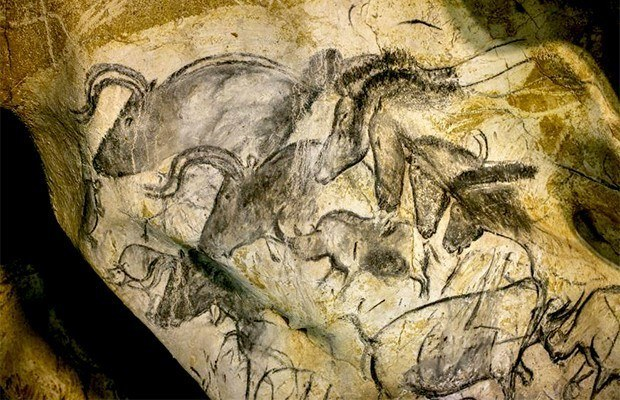
\includegraphics[width=\paperwidth,height=\paperheight]{Imagens/rupestre.jpg}
	}
	
	% Frame 3: plano de fundo
	\begin{frame}
		
		
		\flushleft\color{yellow}{\Huge Paleolítico }
		
	\end{frame}
}

{%
	\usebackgroundtemplate{
		\centering
		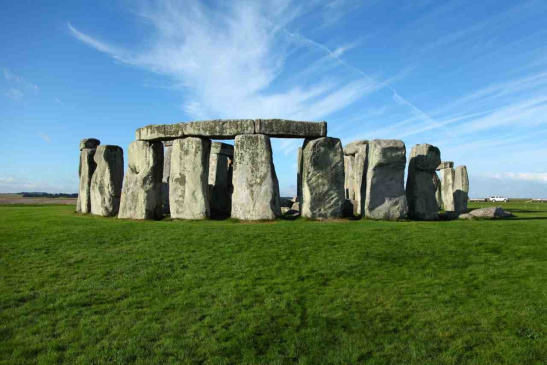
\includegraphics[width=\paperwidth,height=\paperheight]{Imagens/stonerange.jpg}
	}
	
	% Frame 3: plano de fundo
	\begin{frame}
		
		\flushbottom\color{yellow}{\Huge Neolítico}
		
	\end{frame}
}

\begin{frame}
	\frametitle{Introdução}
	\transboxin%efeito de transição	
	\begin{block}{Por que utilizar o redes neuronais?}
		\begin{itemize}
			\pause
			\item Estratégia computacional para a solução de problemas cujo reconhecimento de padrões seja o foco principal \citep{MacKay2005};
			\pause
			\item Capacidade de melhorarem a si próprios automaticamente \citep{Michie1994,Levy1997};
			\pause
			\item Permite lidar com uma grande quantidade de informação \citep{Mao1996,Hall2014}.
		\end{itemize}	
	\end{block}
	
\end{frame}
\subsection{O que vem a ser uma rede neuronal artificial?}
\begin{frame}
	\frametitle{O que vem a ser uma rede neuronal artificial?}
				\pause
				\color{blue} É um sistema artificial que visa simular numericamente os processos do relizados pelo sistema nervoso central. 
				\pause
				\begin{itemize}
					\item Disponta como uma alternativa ao paradigma computacional de Von Neumann (instruções de programação sequencial);
					\pause
					\item Inspirada na neurociência, contudo não é realística em detalhe;
					\pause
					\item Métodos são derivados da Física Estatística;
					\pause
					\item Aplicações em ciência da computação, engenharia, geologia e geofísica. 
				\end{itemize}
\end{frame}

\begin{frame}
	\frametitle{O cérebro humano contém cerca de \\ aproximadamente $10^{11}$  neurônios}
	\begin{figure}
		\centering
		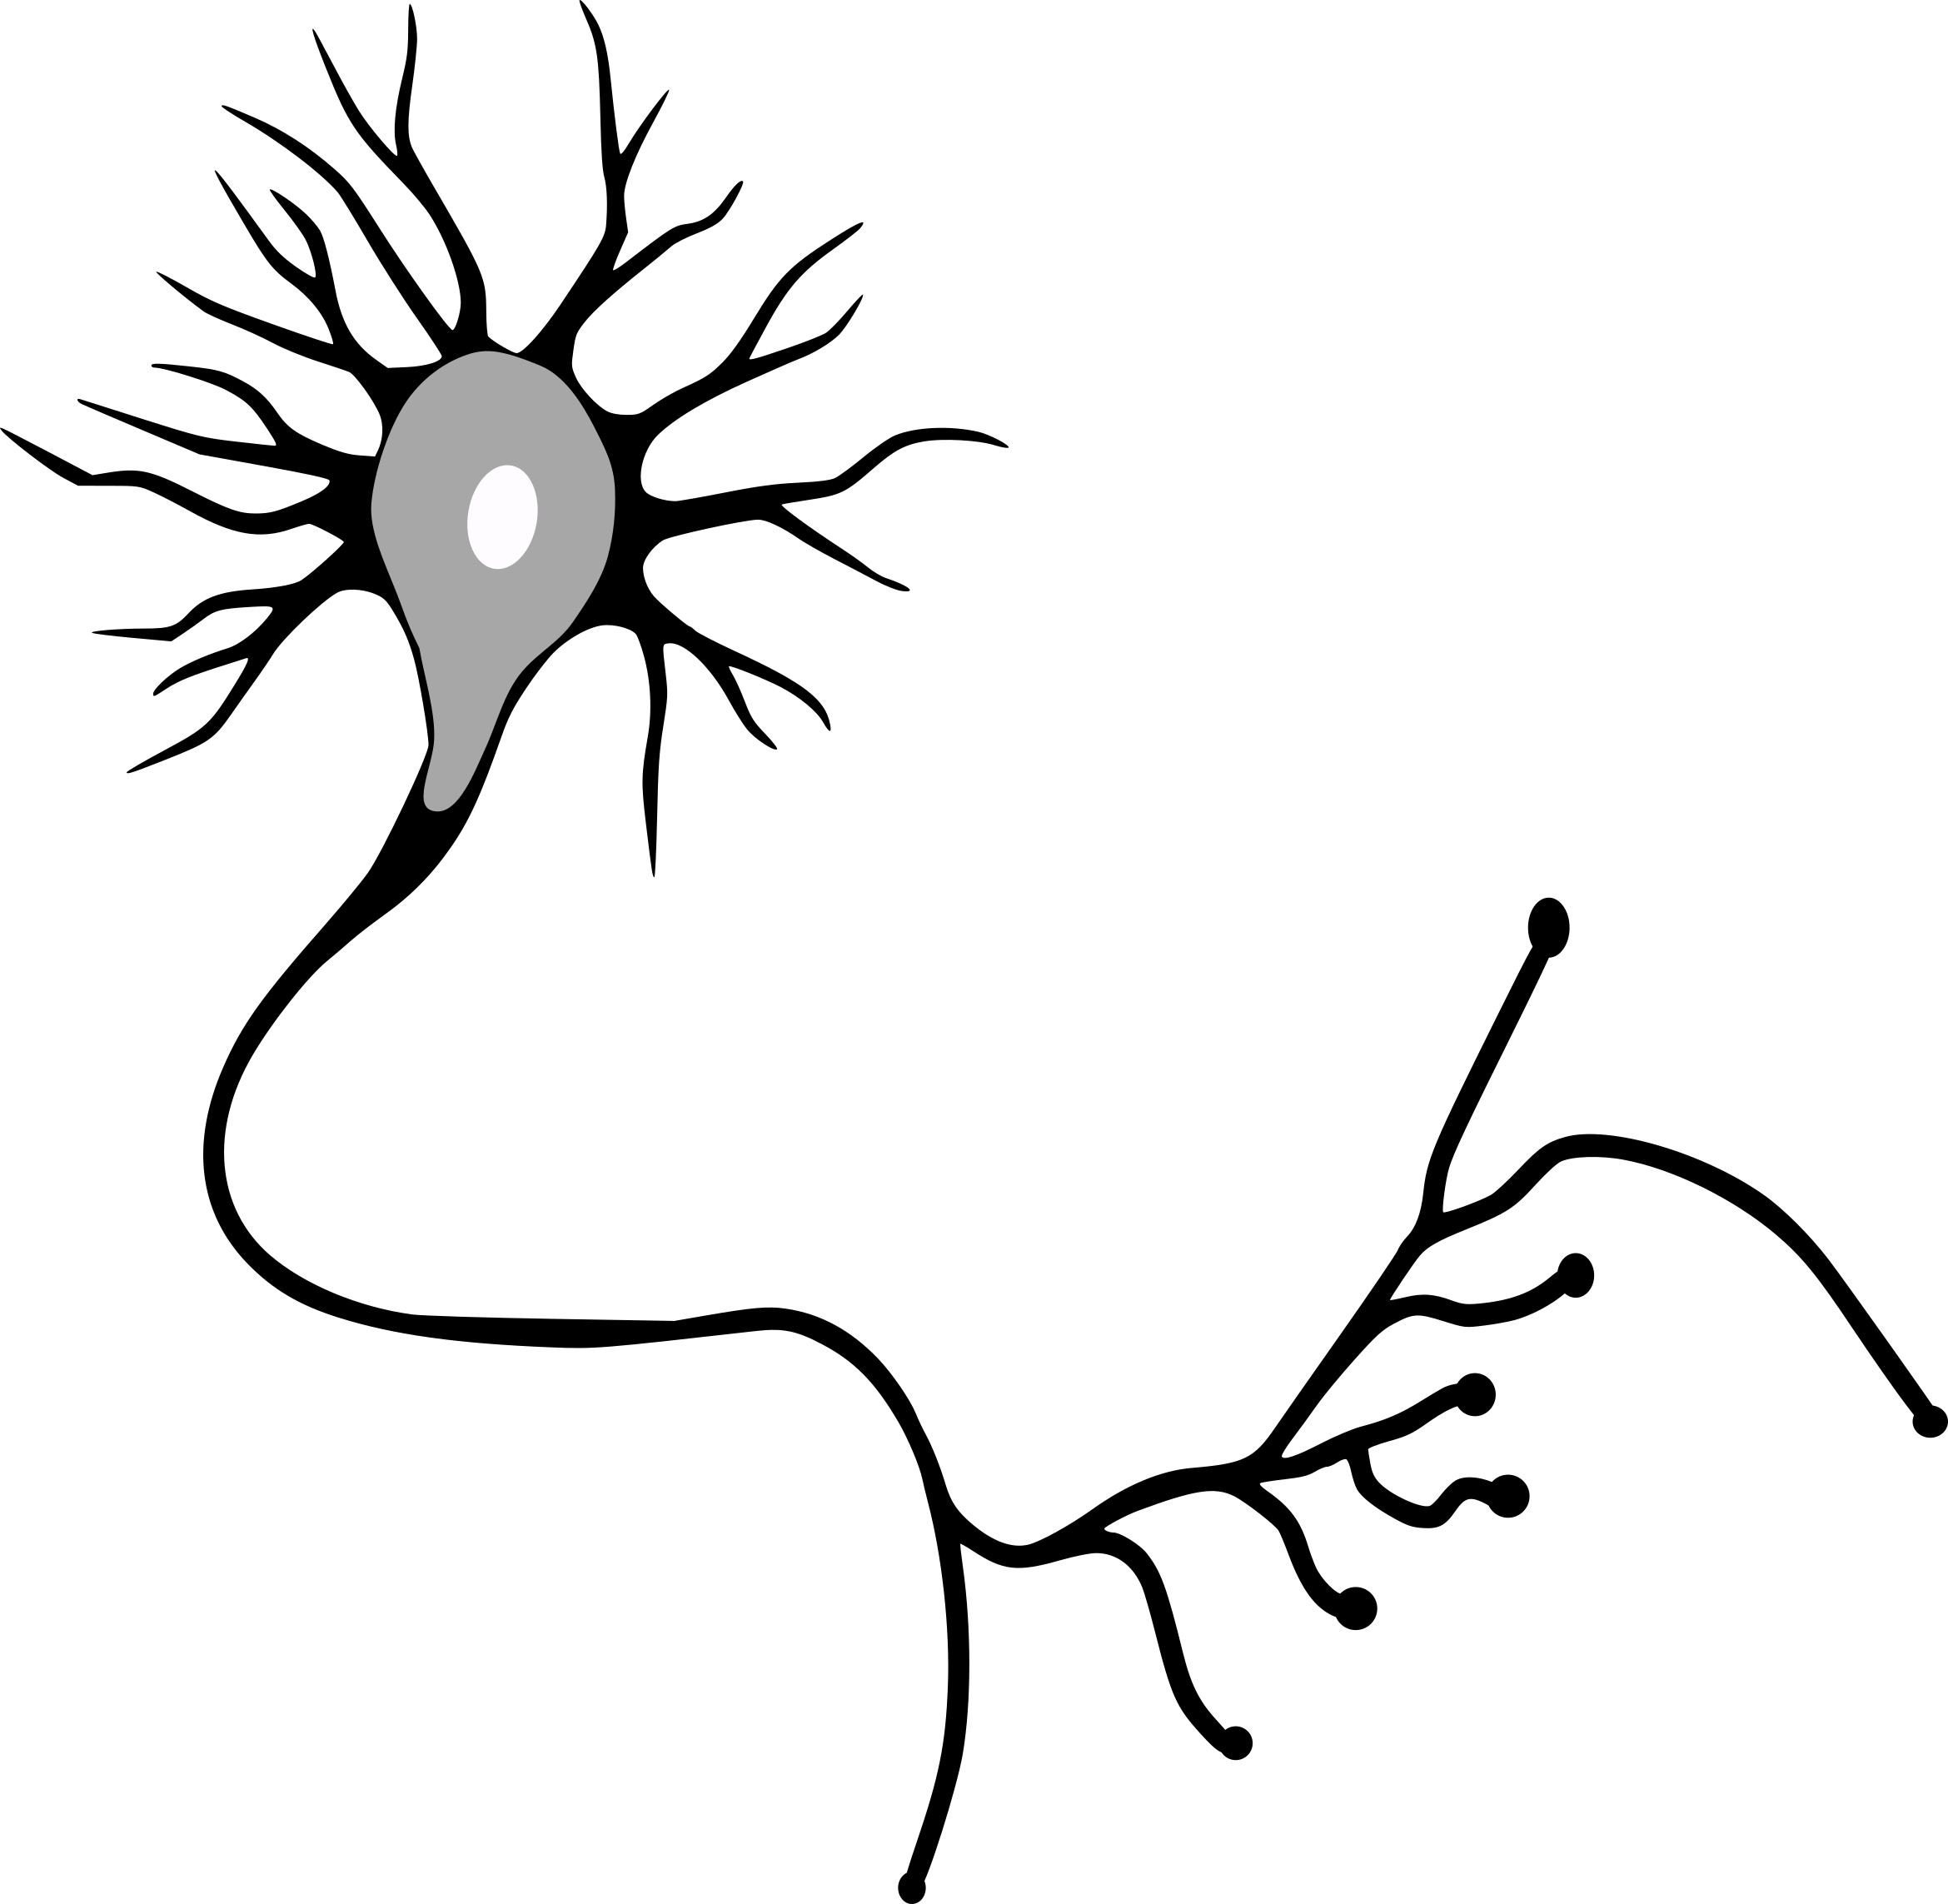
\includegraphics[scale=0.2]{Imagens/neuronio.png} 
		\caption{Ilustração esquemática de um neurônio.}
	\end{figure}
\end{frame}

\begin{frame}
	\frametitle{O cérebro humano contém cerca de \\ aproximadamente $10^{11}$   neurônios}
	\begin{figure}
		\centering
		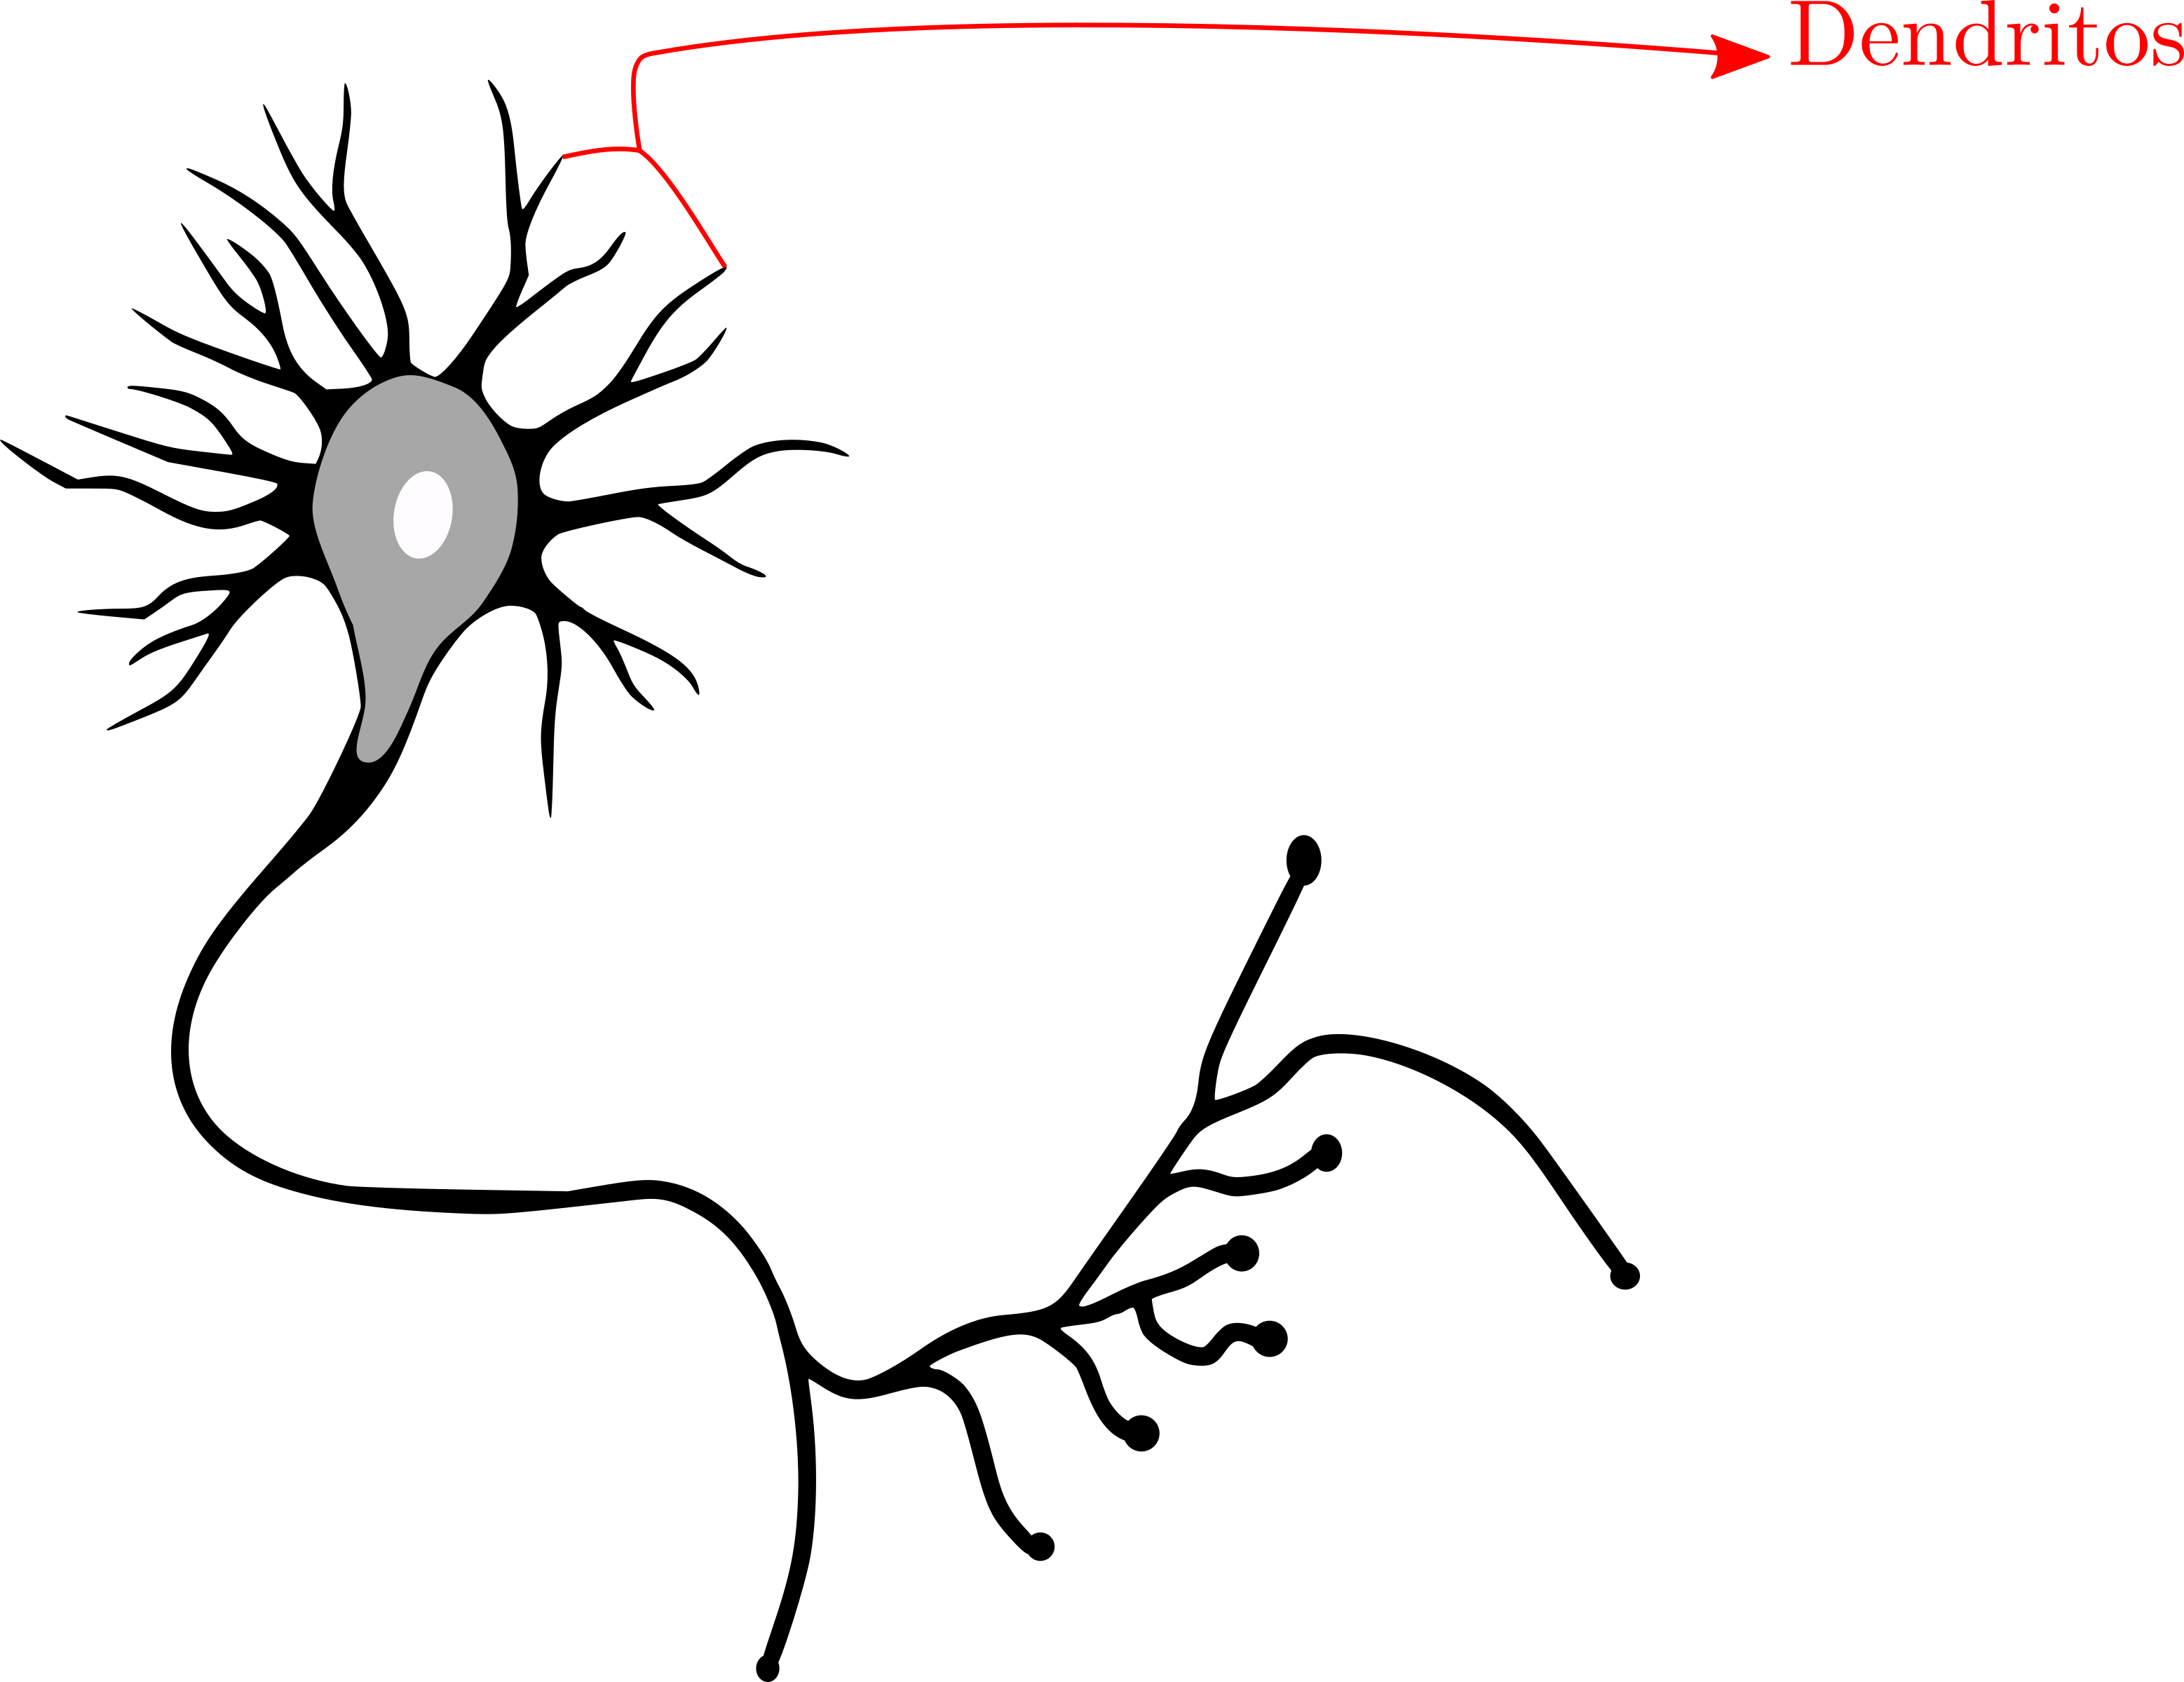
\includegraphics[scale=0.2]{Imagens/dendrito.png} 
		\caption{Ilustração esquemática de um neurônio.}
	\end{figure}
\end{frame}

\begin{frame}
	\frametitle{O cérebro humano contém cerca de \\ aproximadamente $10^{11}$   neurônios}
	\begin{figure}
		\centering
		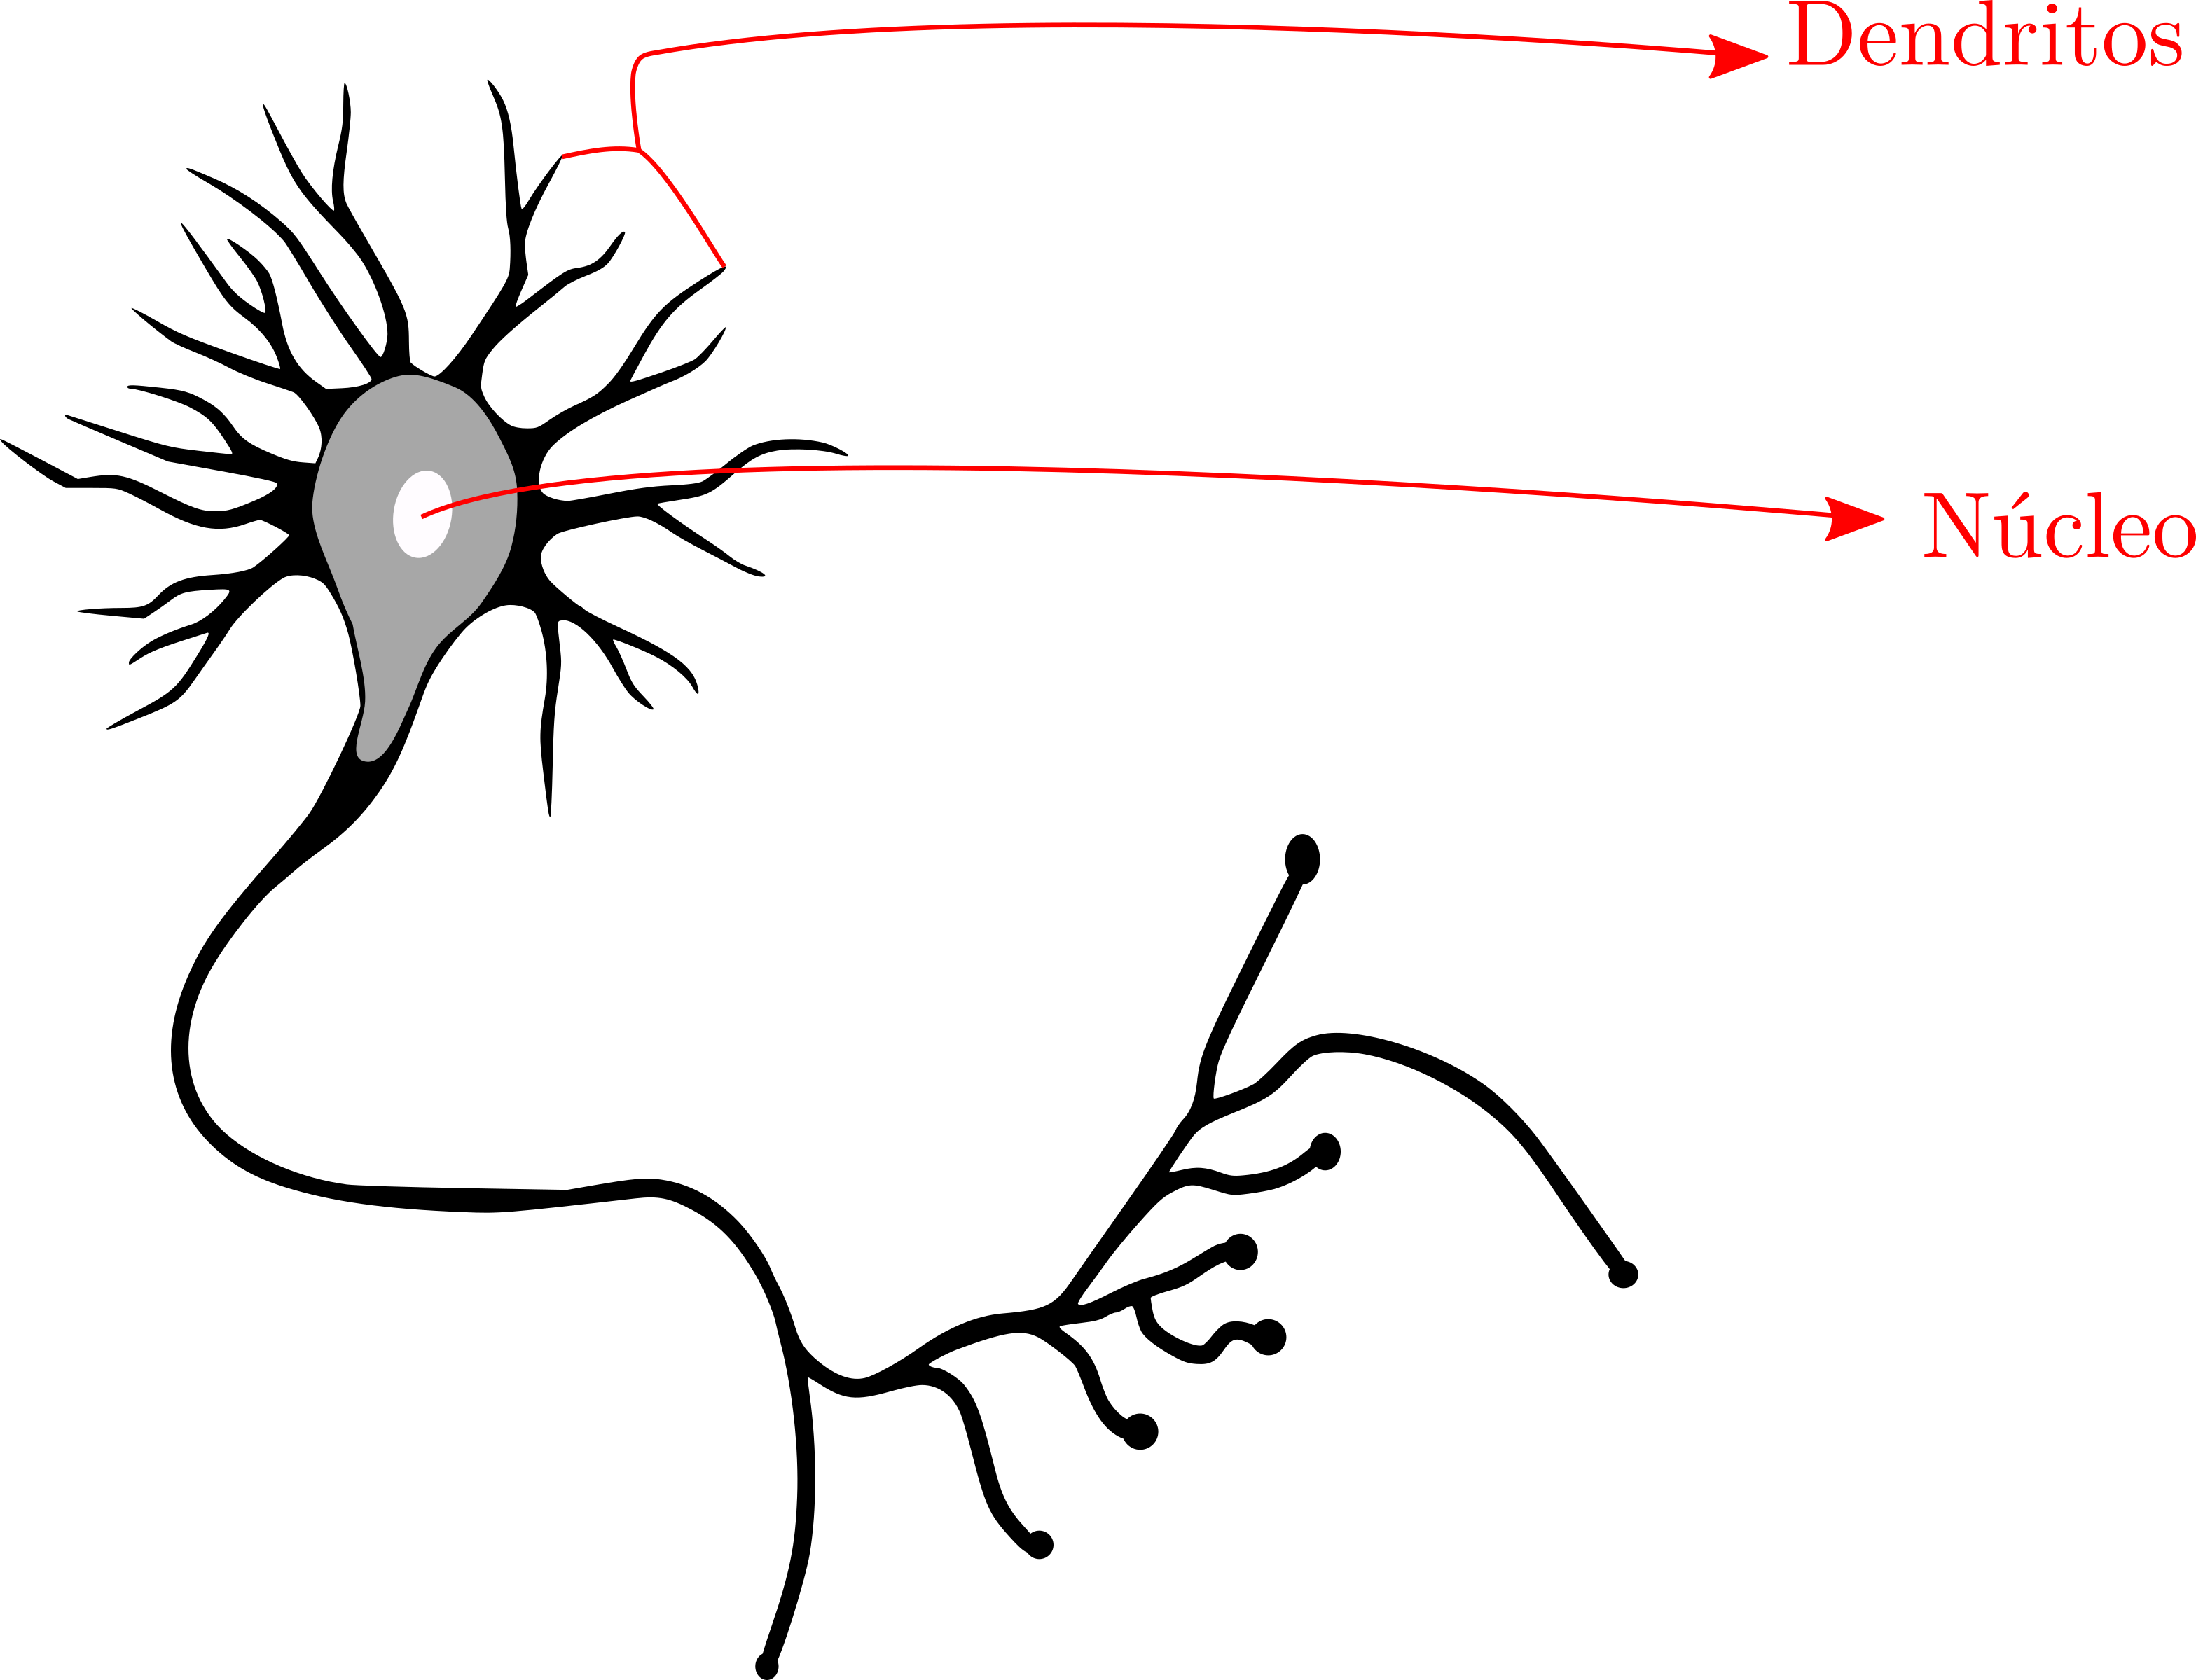
\includegraphics[scale=0.2]{Imagens/nucleo.png} 
		\caption{Ilustração esquemática de um neurônio.}
	\end{figure}
\end{frame}

\begin{frame}
	\frametitle{O cérebro humano contém cerca de \\ aproximadamente $10^{11}$   neurônios}
	\begin{figure}
		\centering
		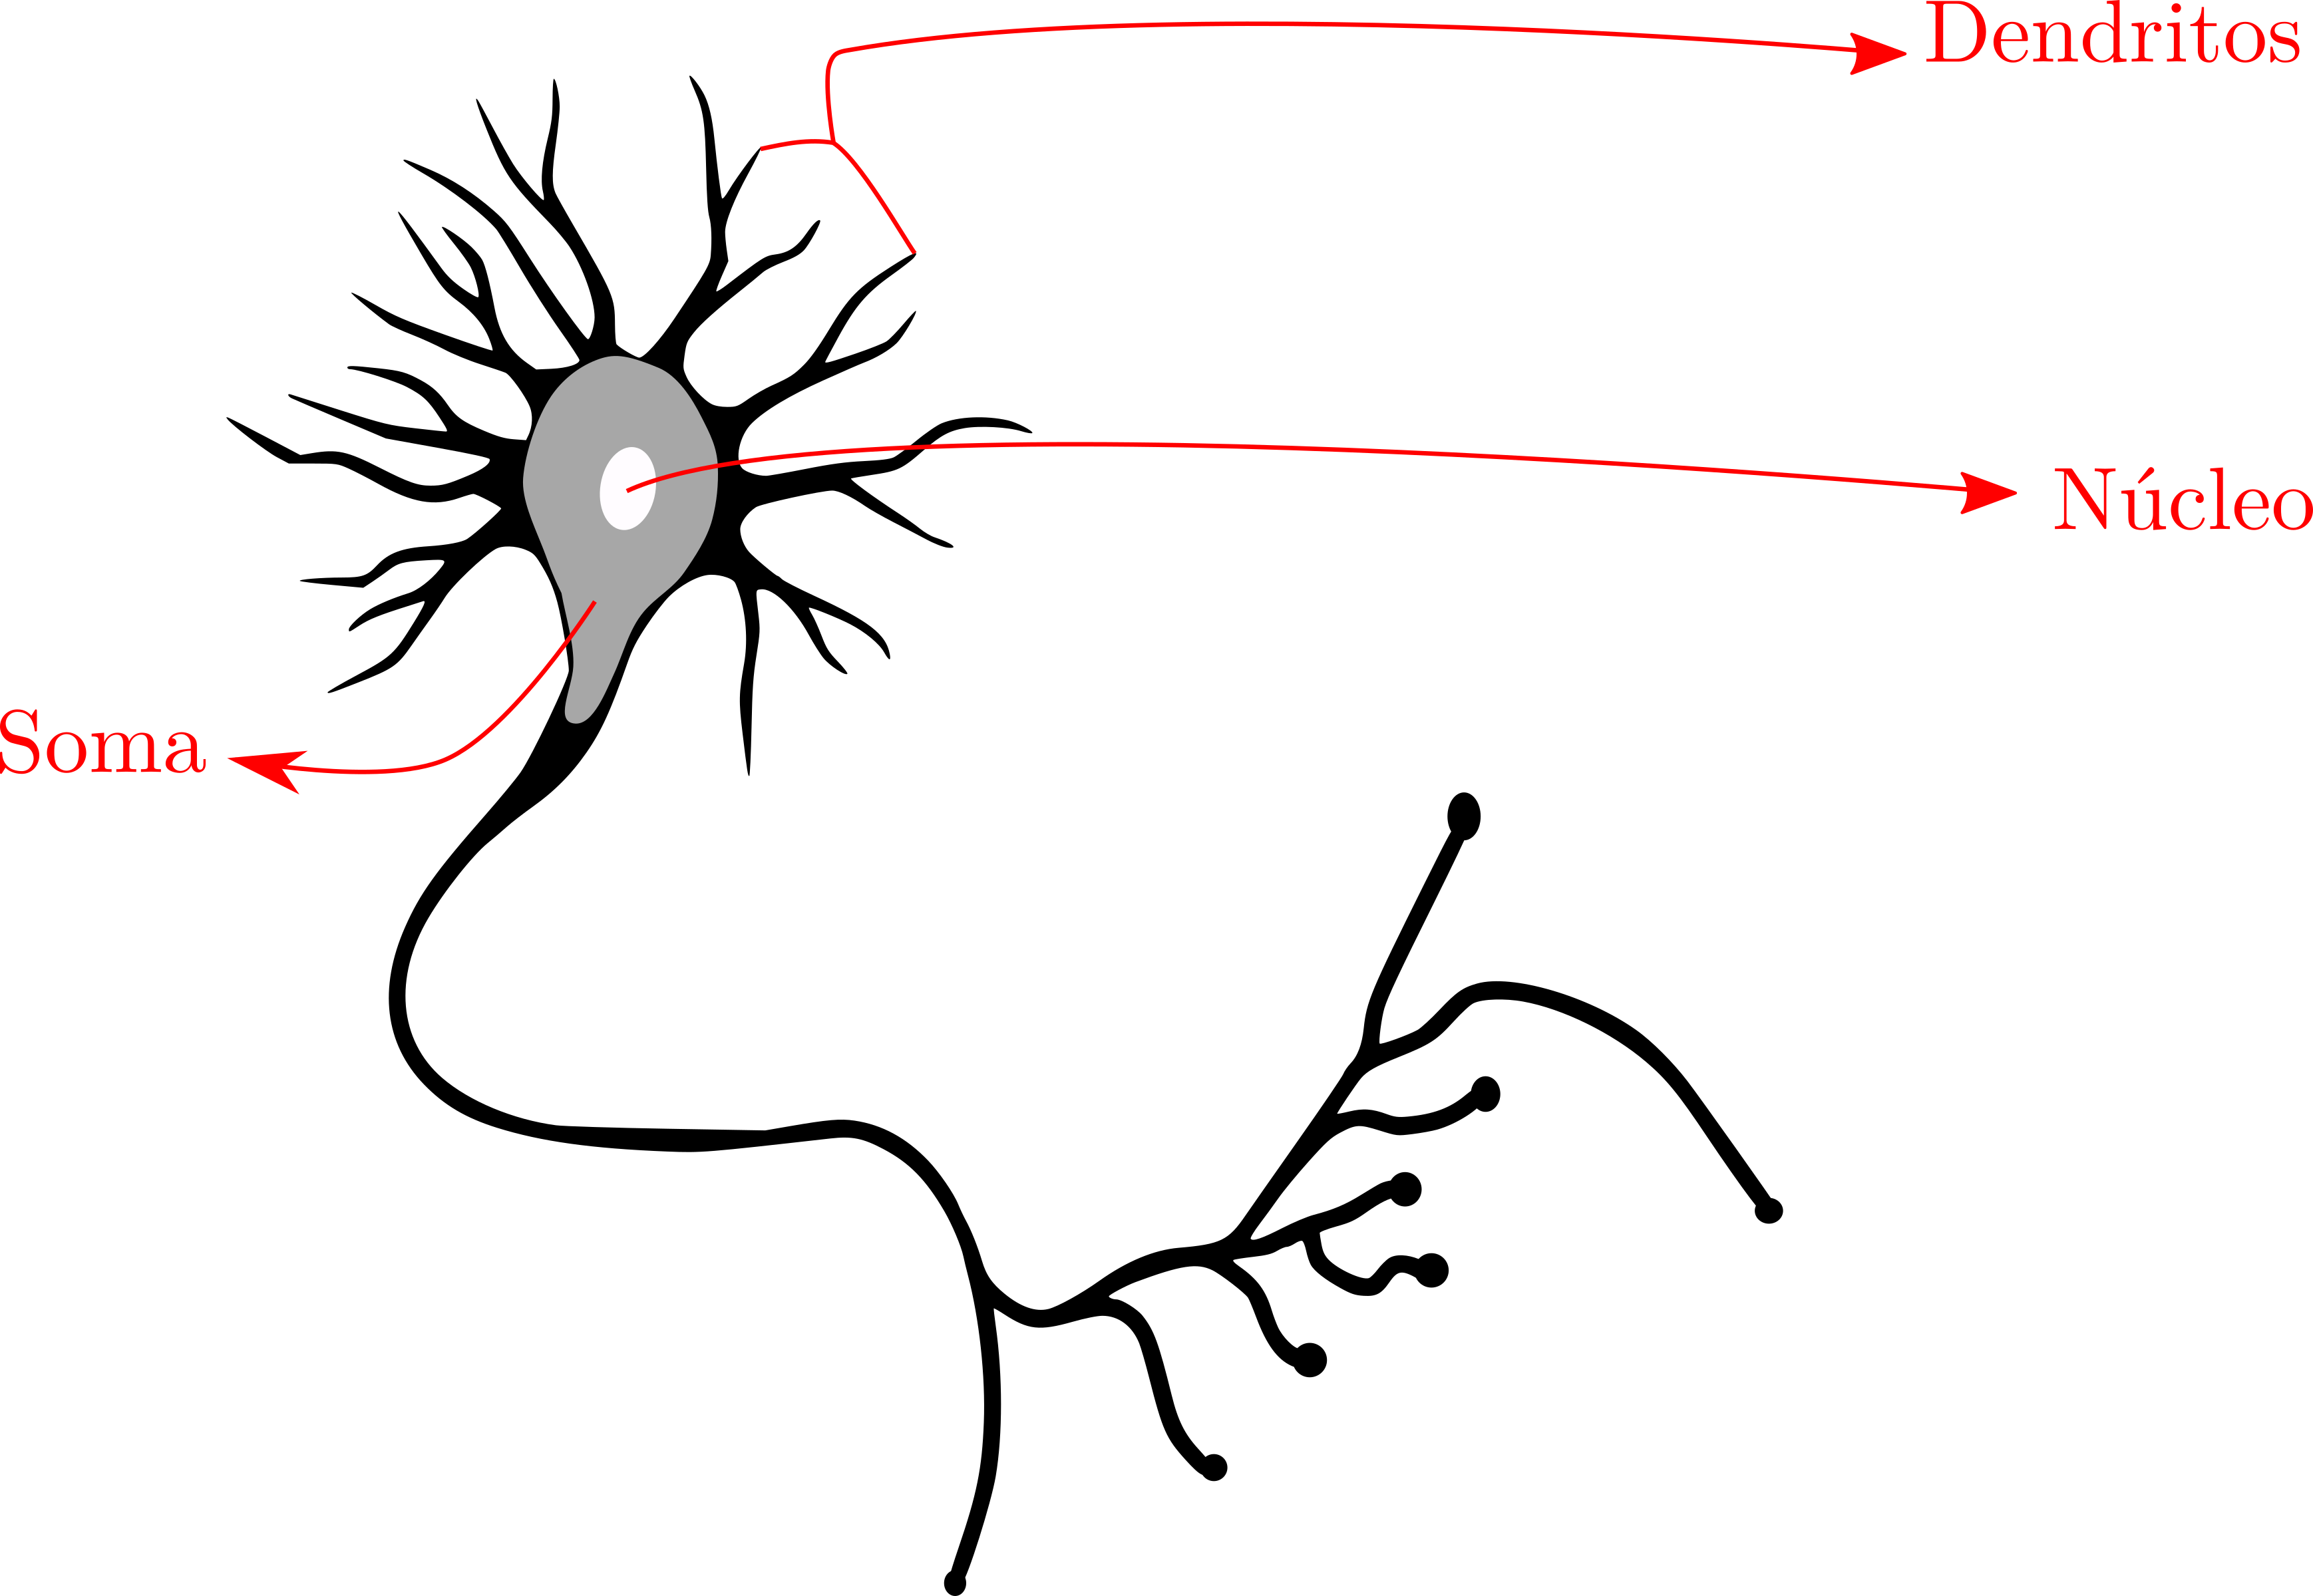
\includegraphics[scale=0.2]{Imagens/soma.png} 
		\caption{Ilustração esquemática de um neurônio.}
	\end{figure}
\end{frame}


\begin{frame}
	\frametitle{O cérebro humano contém cerca de \\ aproximadamente $10^{11}$   neurônios}
	\begin{figure}
		\centering
		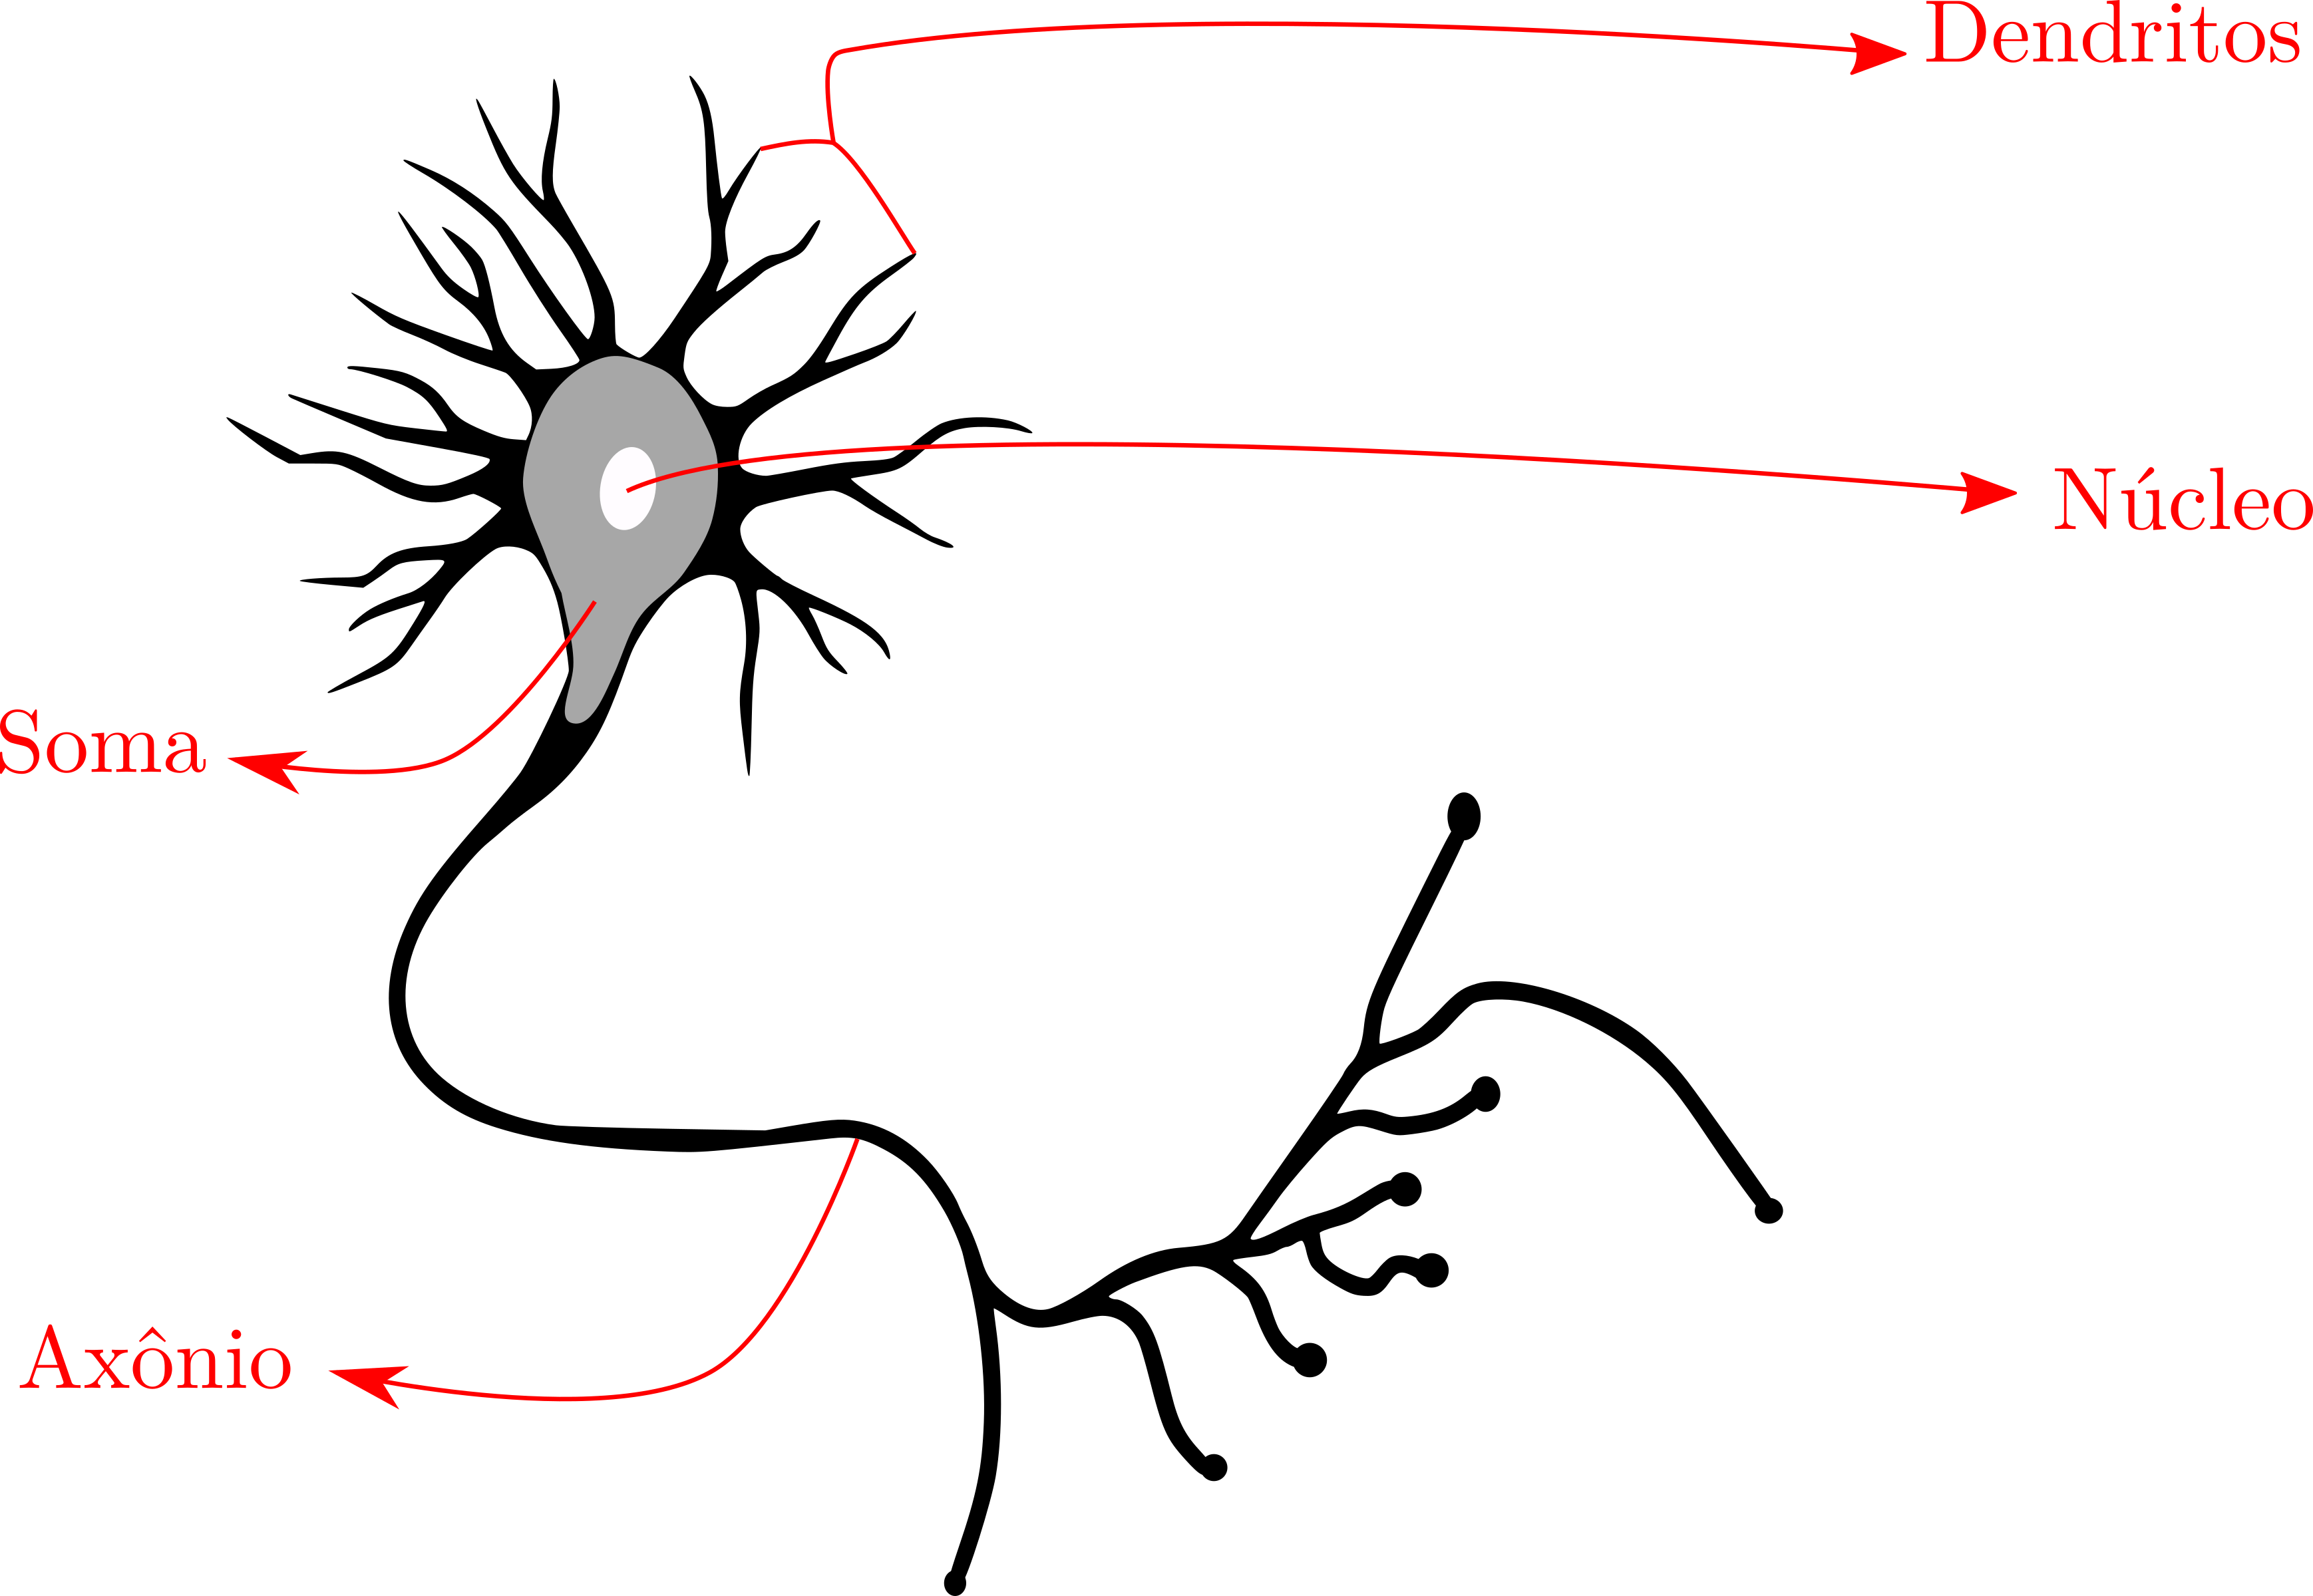
\includegraphics[scale=0.2]{Imagens/axonio.png} 
		\caption{Ilustração esquemática de um neurônio.}
	\end{figure}
\end{frame}

\begin{frame}
	\frametitle{O cérebro humano contém cerca de \\ aproximadamente $10^{11}$   neurônios}
	\begin{figure}
		\centering
		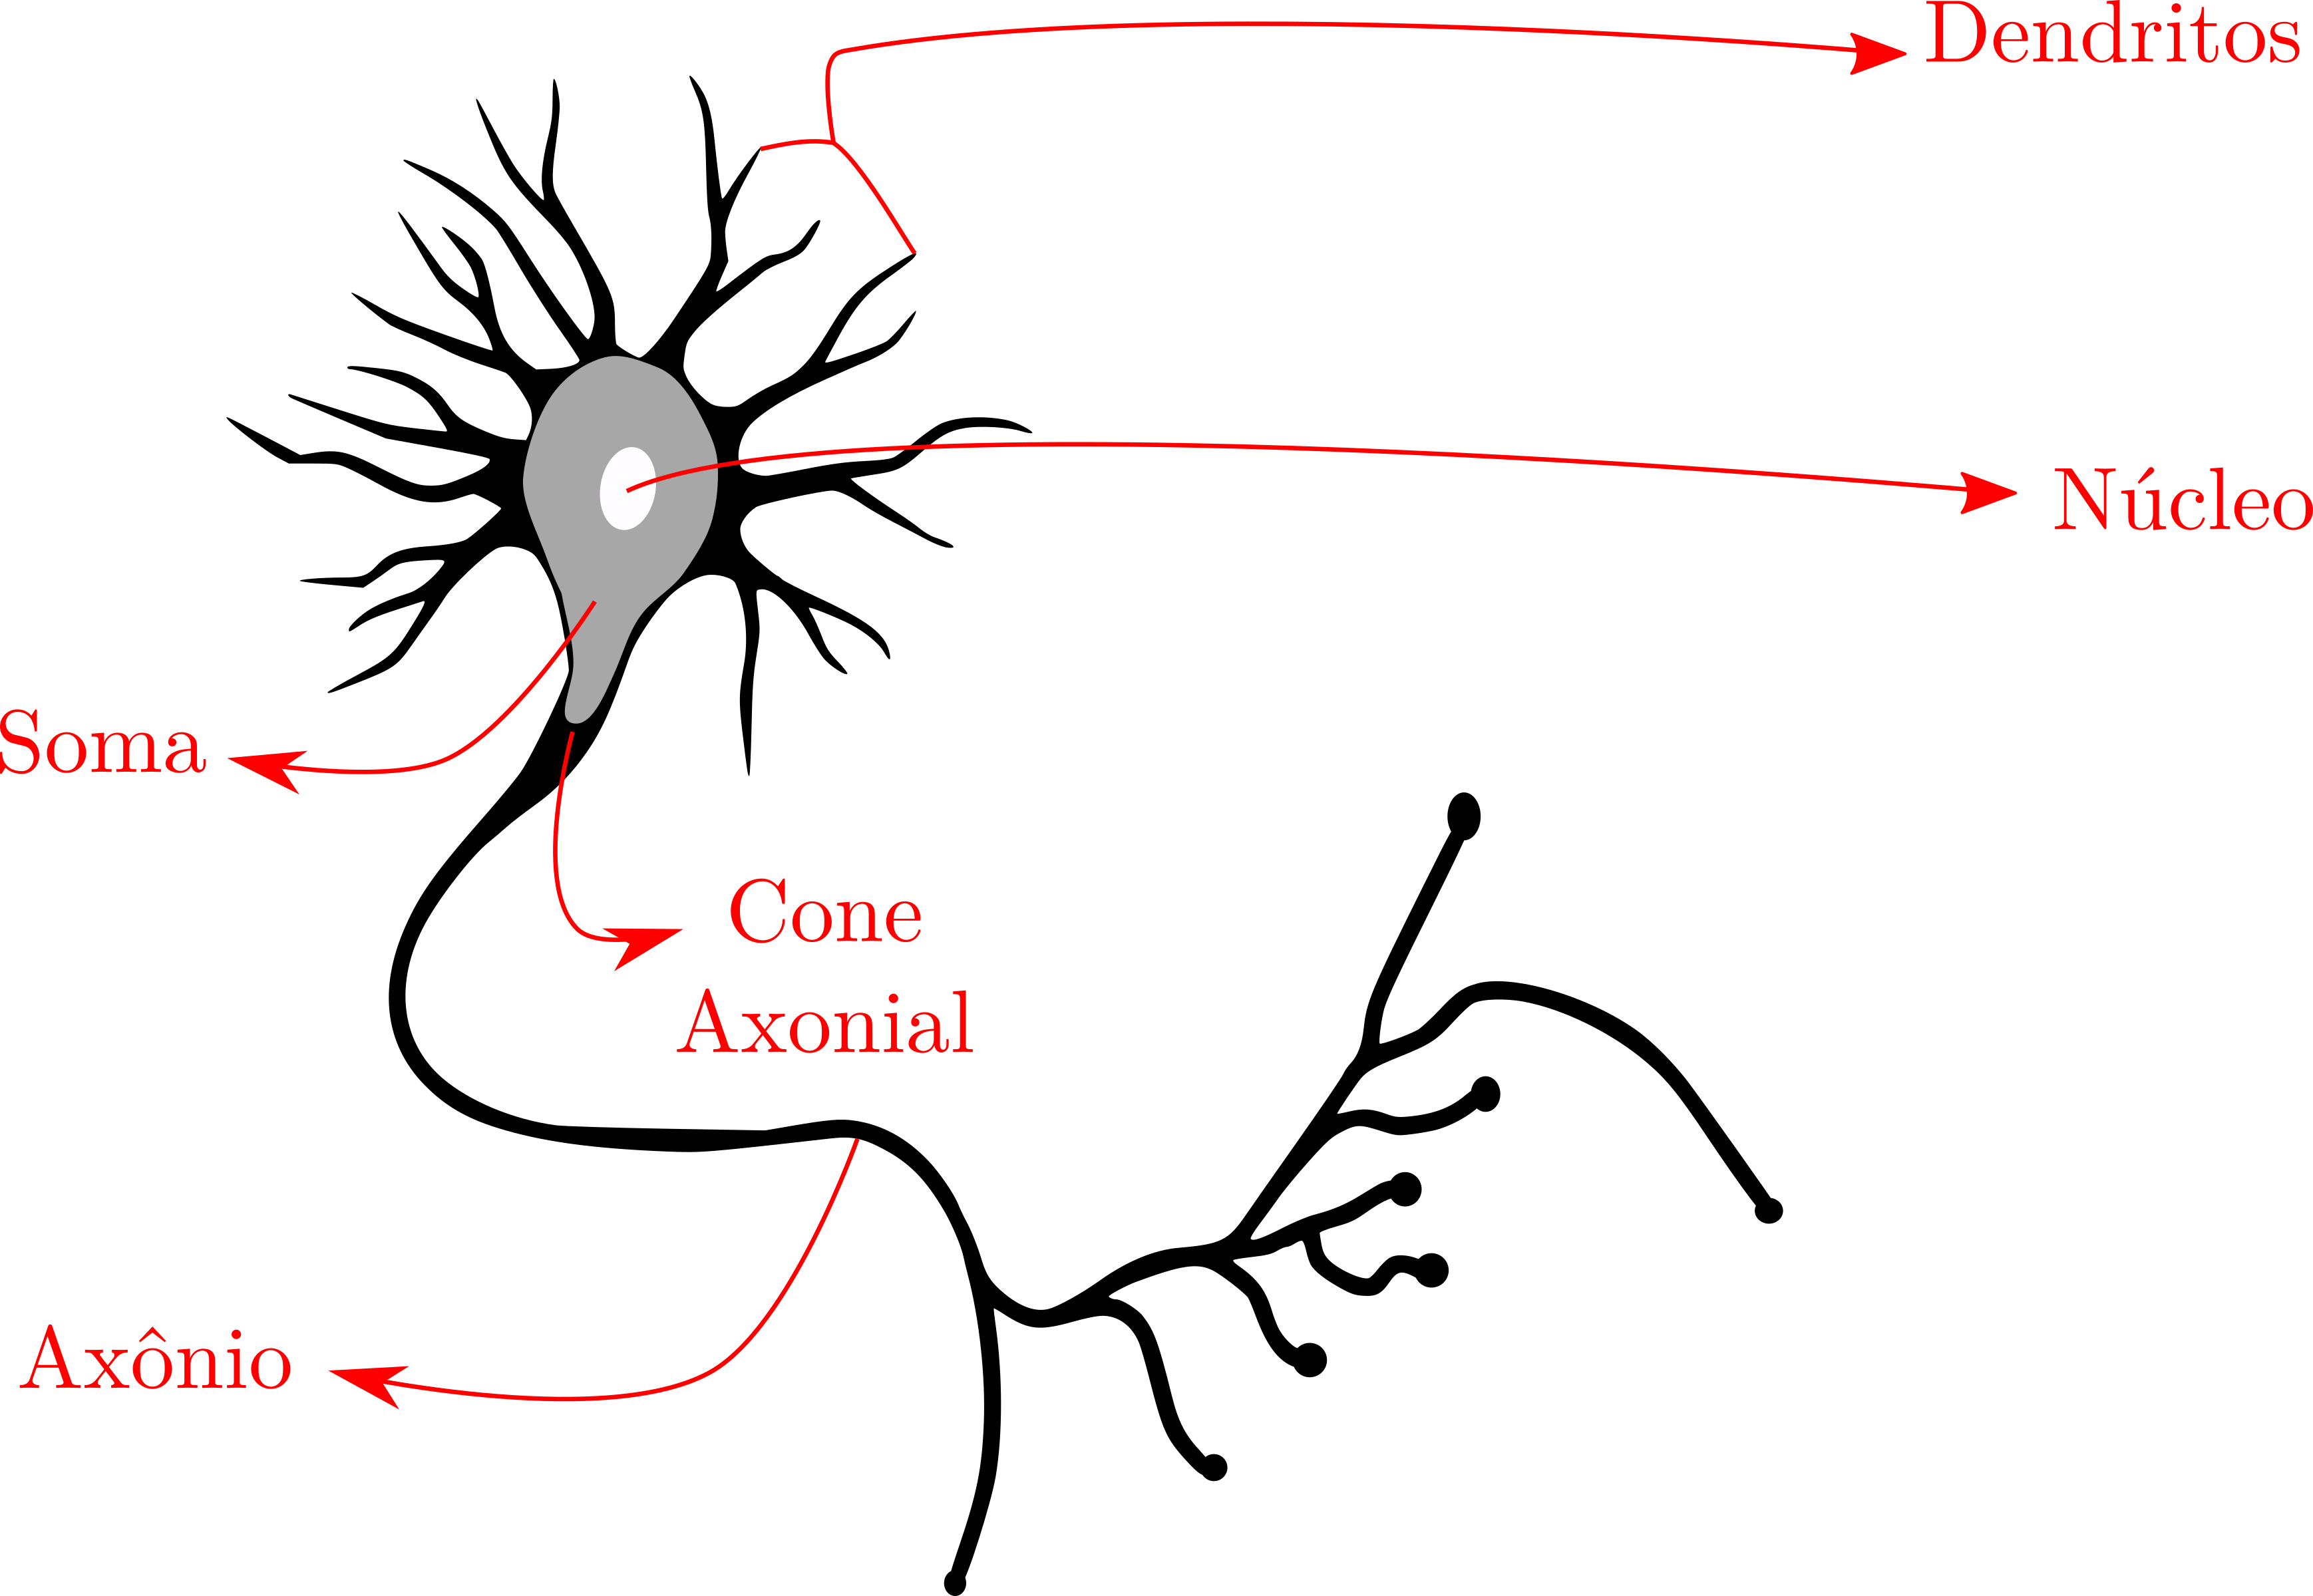
\includegraphics[scale=0.2]{Imagens/cone.png} 
		\caption{Ilustração esquemática de um neurônio.}
	\end{figure}
\end{frame}

\begin{frame}
	\frametitle{O cérebro humano contém cerca de \\ aproximadamente $10^{11}$   de vários tipos}
	\begin{figure}
		\centering
		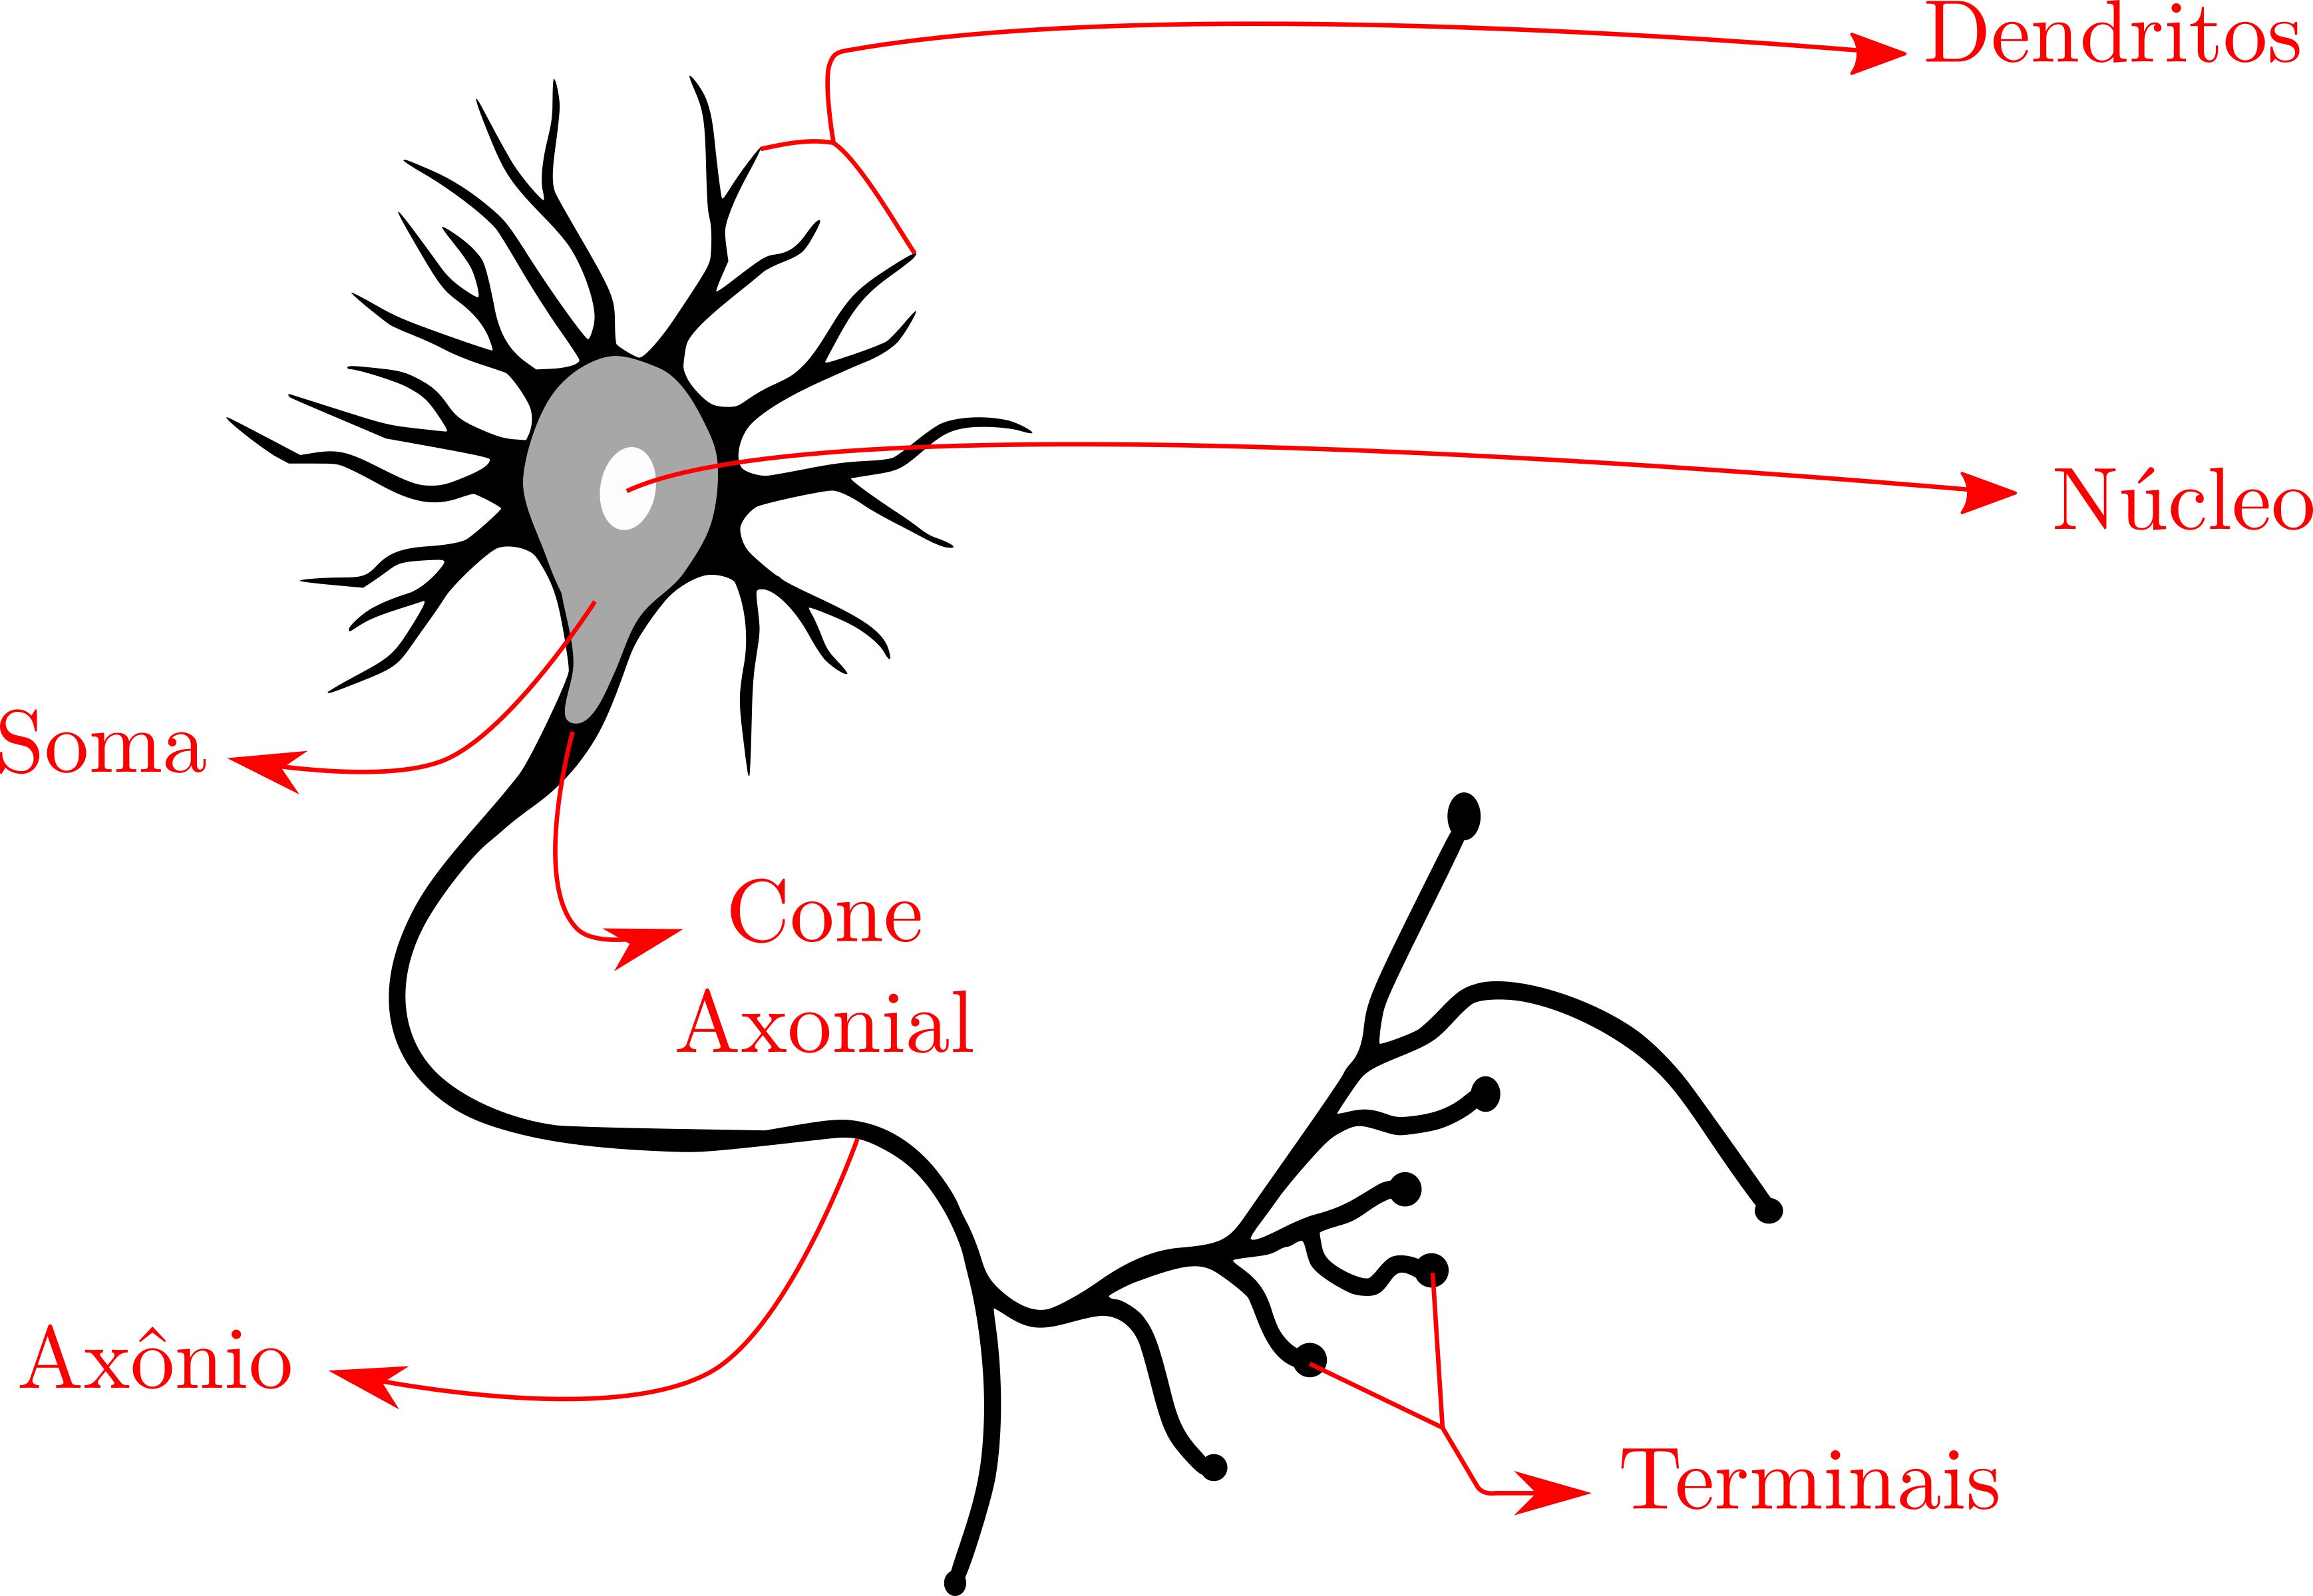
\includegraphics[scale=0.2]{Imagens/terminal.png} 
		\caption{Ilustração esquemática de um neurônio.}
	\end{figure}
\end{frame}

\subsection{Um breve histórico}

\begin{frame}
	\frametitle{Um breve histórico...}
	\pause
	\begin{small}
			\smartdiagram[flow diagram:horizontal]{\textcolor{blue}{\cite{McCulloch1943}}}
	\end{small}
	\begin{itemize}
	\item Definem o a função do neurônio numérico cuja a resposta dependia da entrada dos dados da rede e dos pesos utilizados e a denominam como Perceptron.
	\end{itemize}	
\end{frame}


\begin{frame}
	\frametitle{Um breve histórico...}
	\begin{small}
		\smartdiagram[flow diagram:horizontal]{\citet{McCulloch1943}, \textcolor{blue}{\citet{Rosenblatt1962}}}
	\end{small}
	\begin{itemize}
		\item Definem teoria de convergência do Perceptron onde ele prova que modelos de neurônios possuem propriedades similares ao cérebro humano.
	\end{itemize}
\end{frame}

\begin{frame}
	\frametitle{Um breve histórico...}
	\begin{small}
		\smartdiagram[flow diagram:horizontal]{\citet{McCulloch1943}, \citet{Rosenblatt1962}, \textcolor{blue}{\cite{Minsky1969}}}
	\end{small}
	\begin{itemize}
		\item Demonstraram que Perceptrons somente resolvem uma classe muito limitada de problemas que podem ser linearizados.
	\end{itemize}
\end{frame}

\begin{frame}
	\frametitle{Um breve histórico...}
	\begin{small}
		\smartdiagram[flow diagram:horizontal]{\citet{McCulloch1943}, \citet{Rosenblatt1962}, \cite{Minsky1969}, \textcolor{blue}{\cite{Hopfield1982}}}
	\end{small}
	\begin{itemize}
		\item Cria um modelo de memória auto-associativa com a habilidade de armazenar e depois recuperar um certo conjunto de padrões no dado.  
		%\item The collective properties of this model produce a content-addressable memory which correctly yields an entire	memory from any subpart of sufficient size.
	\end{itemize}
\end{frame}

\begin{frame}
	\frametitle{Um breve histórico...}
	\begin{small}
		\smartdiagram[flow diagram:horizontal]{\citet{Rosenblatt1962}, \cite{Minsky1969}, \cite{Hopfield1982}, \textcolor{blue}{\cite{Kohonen1989}}}
	\end{small}
	\begin{itemize}
		\item Resolve problemas não-lineares criando uma ferramenta para a análise exploratória de dados geoespaciais multivariados.  
		%\item The collective properties of this model produce a content-addressable memory which correctly yields an entire	memory from any subpart of sufficient size.
	\end{itemize}
\end{frame}


\subsection{Estado da arte}

\begin{frame}
	\frametitle{Estado da arte}
	\framesubtitle{na geofísica}
	\begin{itemize}
		\item \textcolor{red}{entre 1988 e 1994} o foco era em descobrir o que as redes neuronais podem fazer com diferentes tipos de dados. E como preparar esses dados para a utilização na rede e como analisá-los; 
		\pause
		\item \textcolor{red}{entre 1995 até o presente} aplicação se torna mais específica na área da caracterização de reservatórios integrando o resultado da RNA com outros resultados.
	\end{itemize}

	\begin{flushleft}
	\citep{Poulton2002, Artero2009}
	\end{flushleft}
	


\end{frame}

\begin{frame}
	\frametitle{Estado da arte}
	\framesubtitle{na perfilagem de poços}
	\begin{small}
	\smartdiagram[flow diagram:horizontal]{\textcolor{blue}{\cite{Zhang1999}}}
	\end{small}
	\begin{itemize}
	\item Algoritmos baseados em derivadas nas curvas de log não identificam camadas muito finas, ou ruído.
	\end{itemize}
\end{frame}

\begin{frame}
	\frametitle{Estado da arte}
	\framesubtitle{na perfilagem de poços}
	\begin{small}
		\smartdiagram[flow diagram:horizontal]{\cite{Zhang1999},\textcolor{blue}{\cite{Chakravarthy1999}}}
	\end{small}
	%\pause
	\begin{itemize}
		\item consegue através do uso da função radial localizar os limites de camadas em alta definição em dados de log de indução (HDIL).
	\end{itemize}
\end{frame}

\begin{frame}
	\frametitle{Estado da arte}
	\framesubtitle{na perfilagem de poços}
	\begin{small}
		\smartdiagram[flow diagram:horizontal]{\cite{Zhang1999},\cite{Chakravarthy1999}, \textcolor{blue}{\cite{Benaouda1999}}}
	\end{small}
	%\pause
	\begin{itemize}
		\item consegue classificar tipos litológicos em poços parcialmente desmoronados.
	\end{itemize}
\end{frame}

\begin{frame}
	\frametitle{Estado da arte}
	\framesubtitle{na perfilagem de poços}
	\begin{small}
		\smartdiagram[flow diagram:horizontal]{\cite{Zhang1999},\cite{Chakravarthy1999}, \cite{Benaouda1999}, \textcolor{blue}{\cite{Saljooghi2014}}}
	\end{small}
	%\pause
	\begin{itemize}
		\item topo e base de camadas que podem ser associadas com mudanças das propriedades petrofísicas. 
	\end{itemize}
\end{frame}

\begin{frame}
	\frametitle{Estado da arte}
	\framesubtitle{na perfilagem de poços}
	\begin{small}
		\smartdiagram[flow diagram:horizontal]{\cite{Chakravarthy1999}, \cite{Benaouda1999},\cite{Saljooghi2014}, \textcolor{blue}{\cite{Gloaguen2017}} }
	\end{small}
	%\pause
	\begin{itemize}
		\item Chama a atenção para importância relativa das propriedades físicas, em dados de perfilagem de ouro, para a tomada de decisão da rede neuronal. 
	\end{itemize}
\end{frame}

\subsection{A rede de Kohonen}

\begin{frame}
	\frametitle{A rede de Kohonen}
	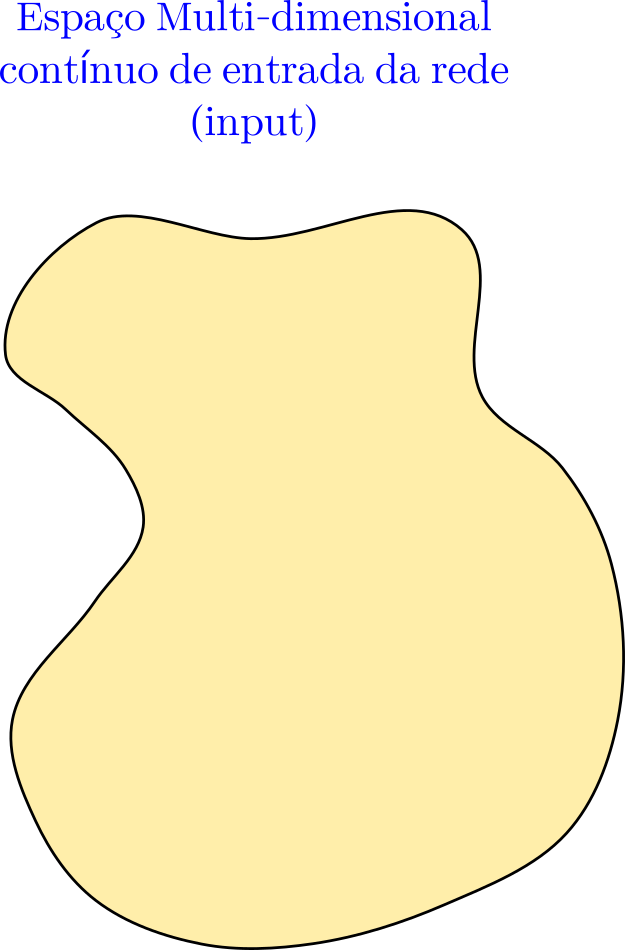
\includegraphics[scale=0.5]{Imagens/IntroKoho1.png} 
	
\end{frame}


\begin{frame}
	\frametitle{A rede de Kohonen}
	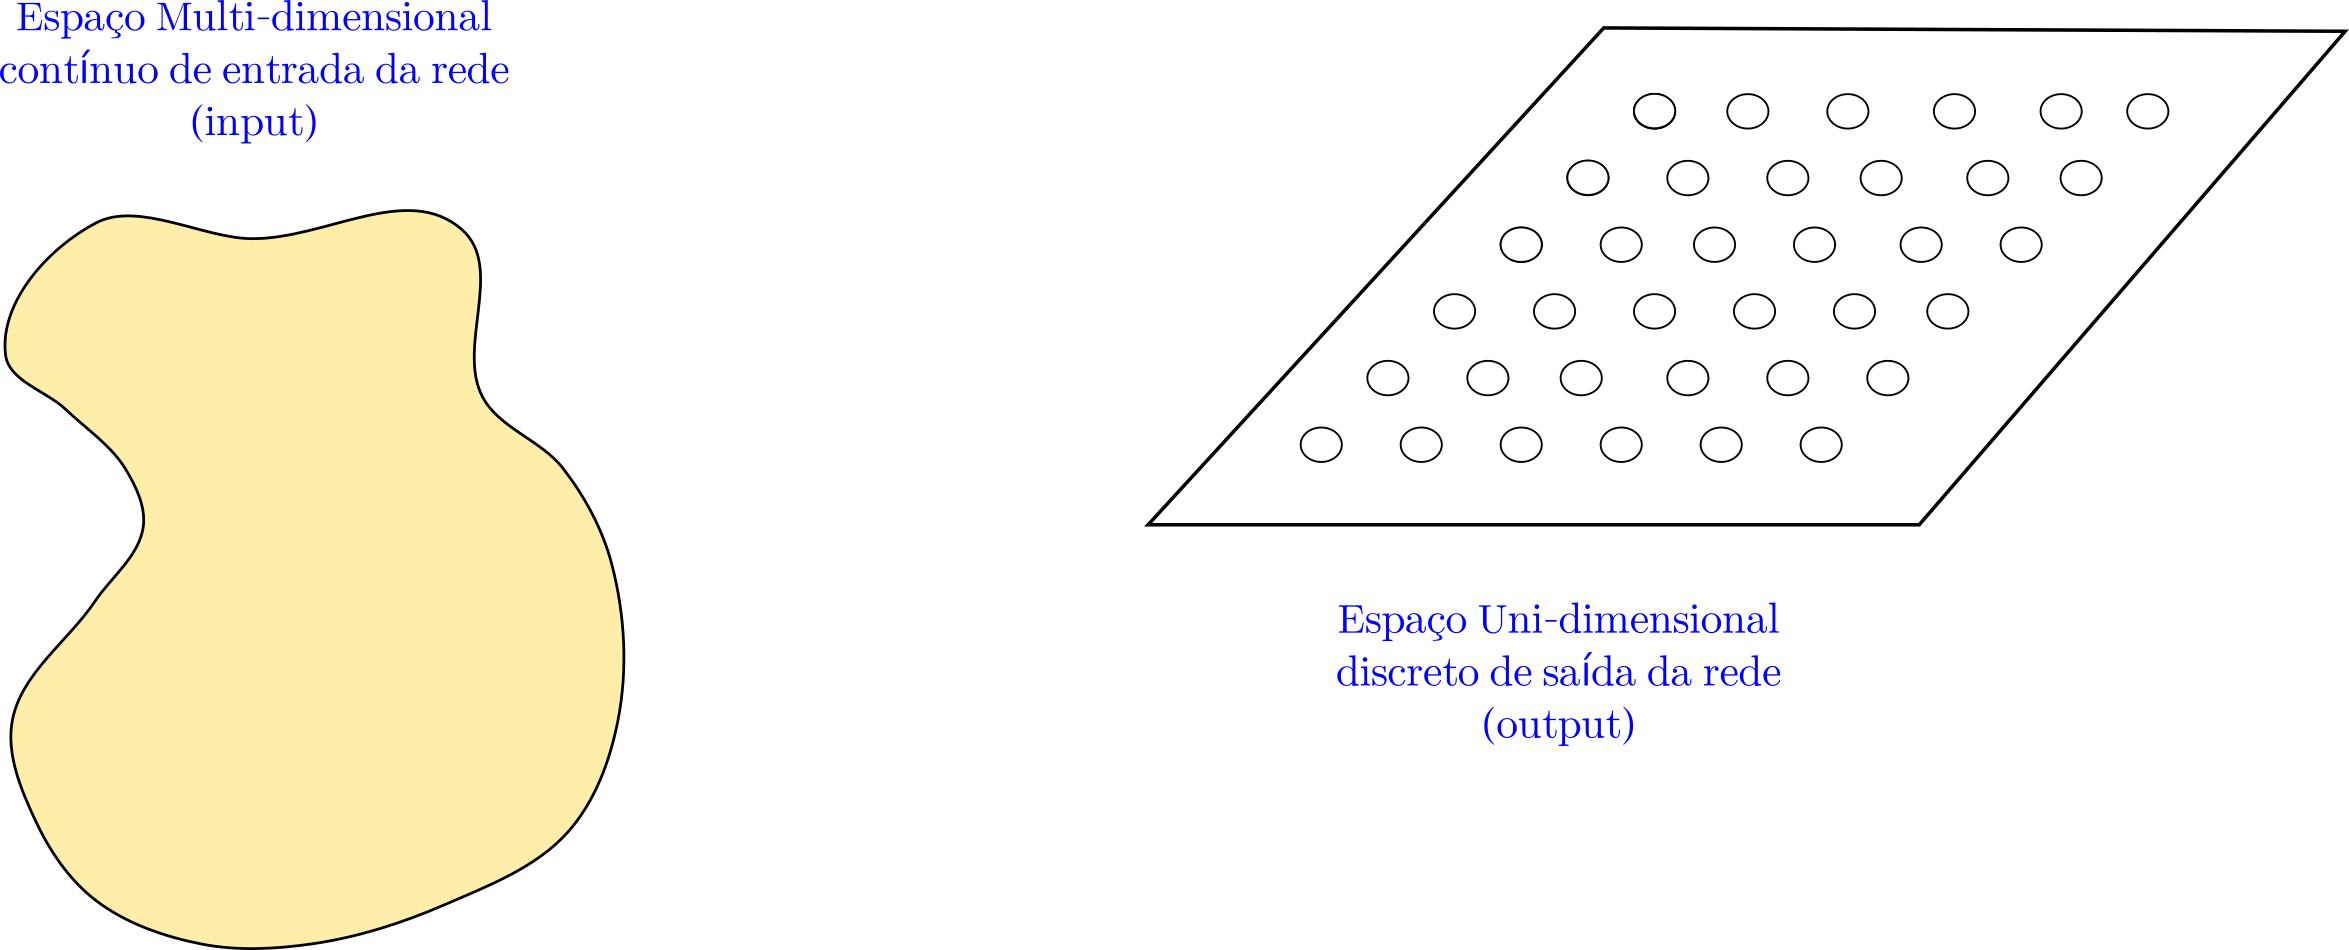
\includegraphics[scale=0.5]{Imagens/IntroKoho2.png} 
	
\end{frame}


\begin{frame}
	\frametitle{A rede de Kohonen}
	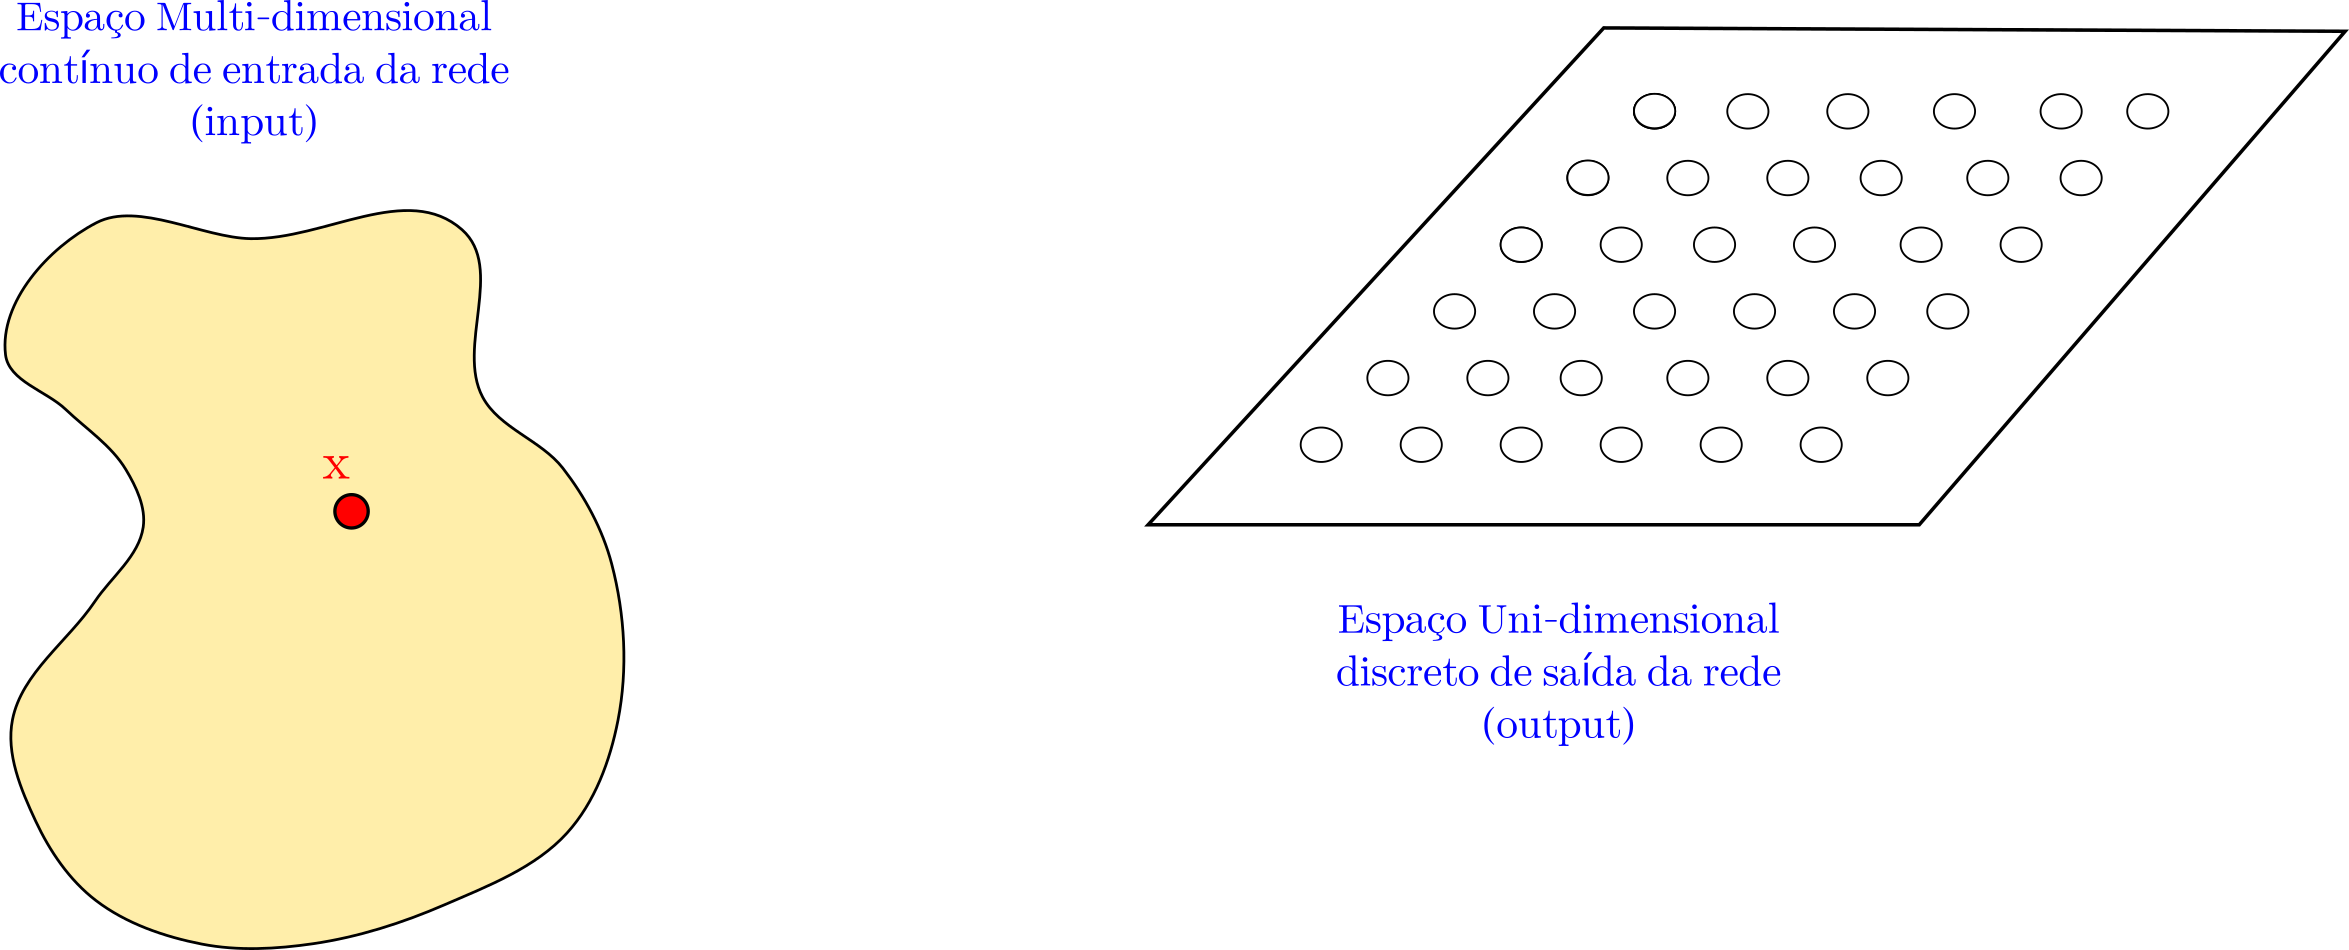
\includegraphics[scale=0.5]{Imagens/IntroKoho3.png} 
	
\end{frame}

\begin{frame}
	\frametitle{A rede de Kohonen}
	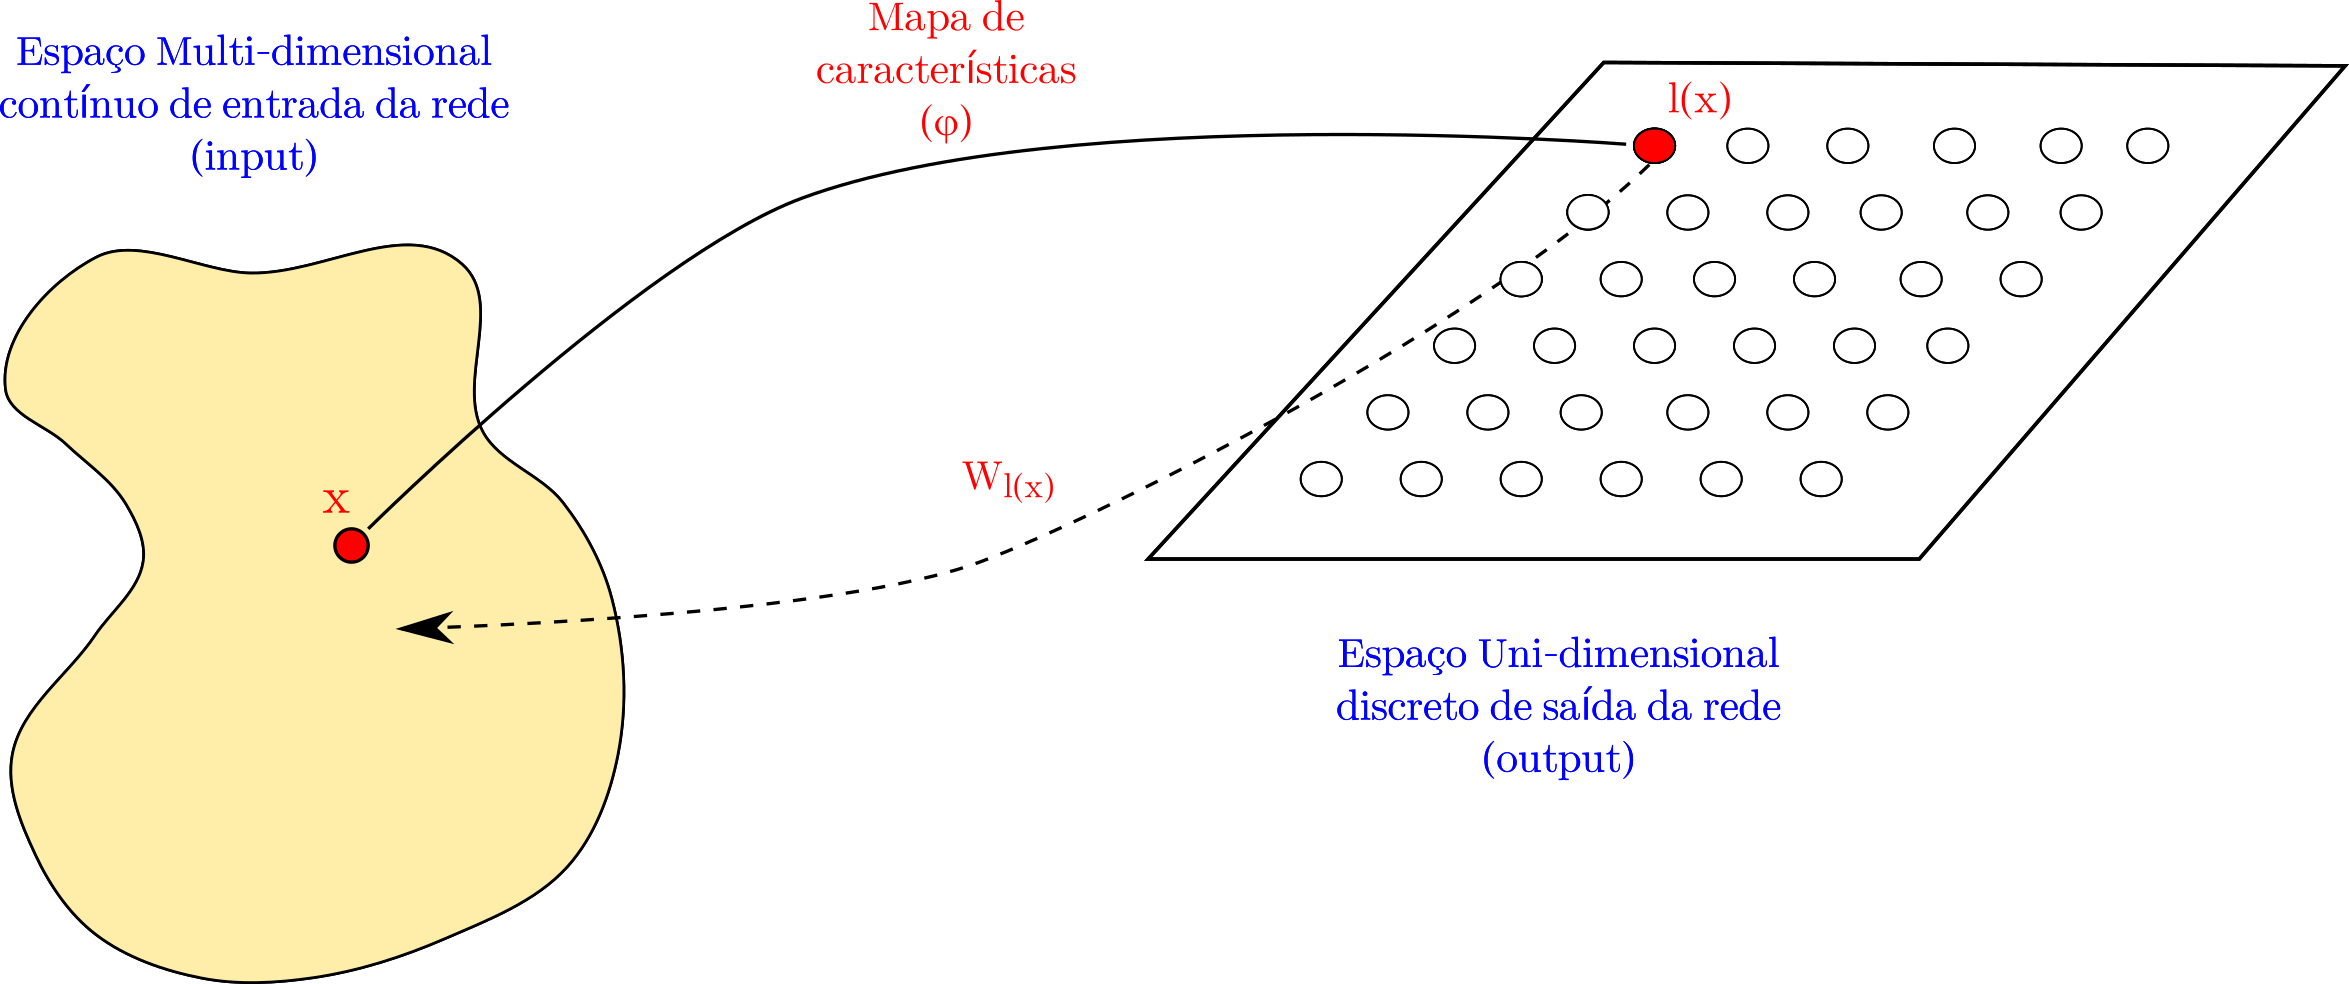
\includegraphics[scale=0.5]{Imagens/IntroKoho4.png} 
	
\end{frame}


\begin{frame}
	\frametitle{A geometria da rede}
	
\begin{figure}[H]
		\flushleft
		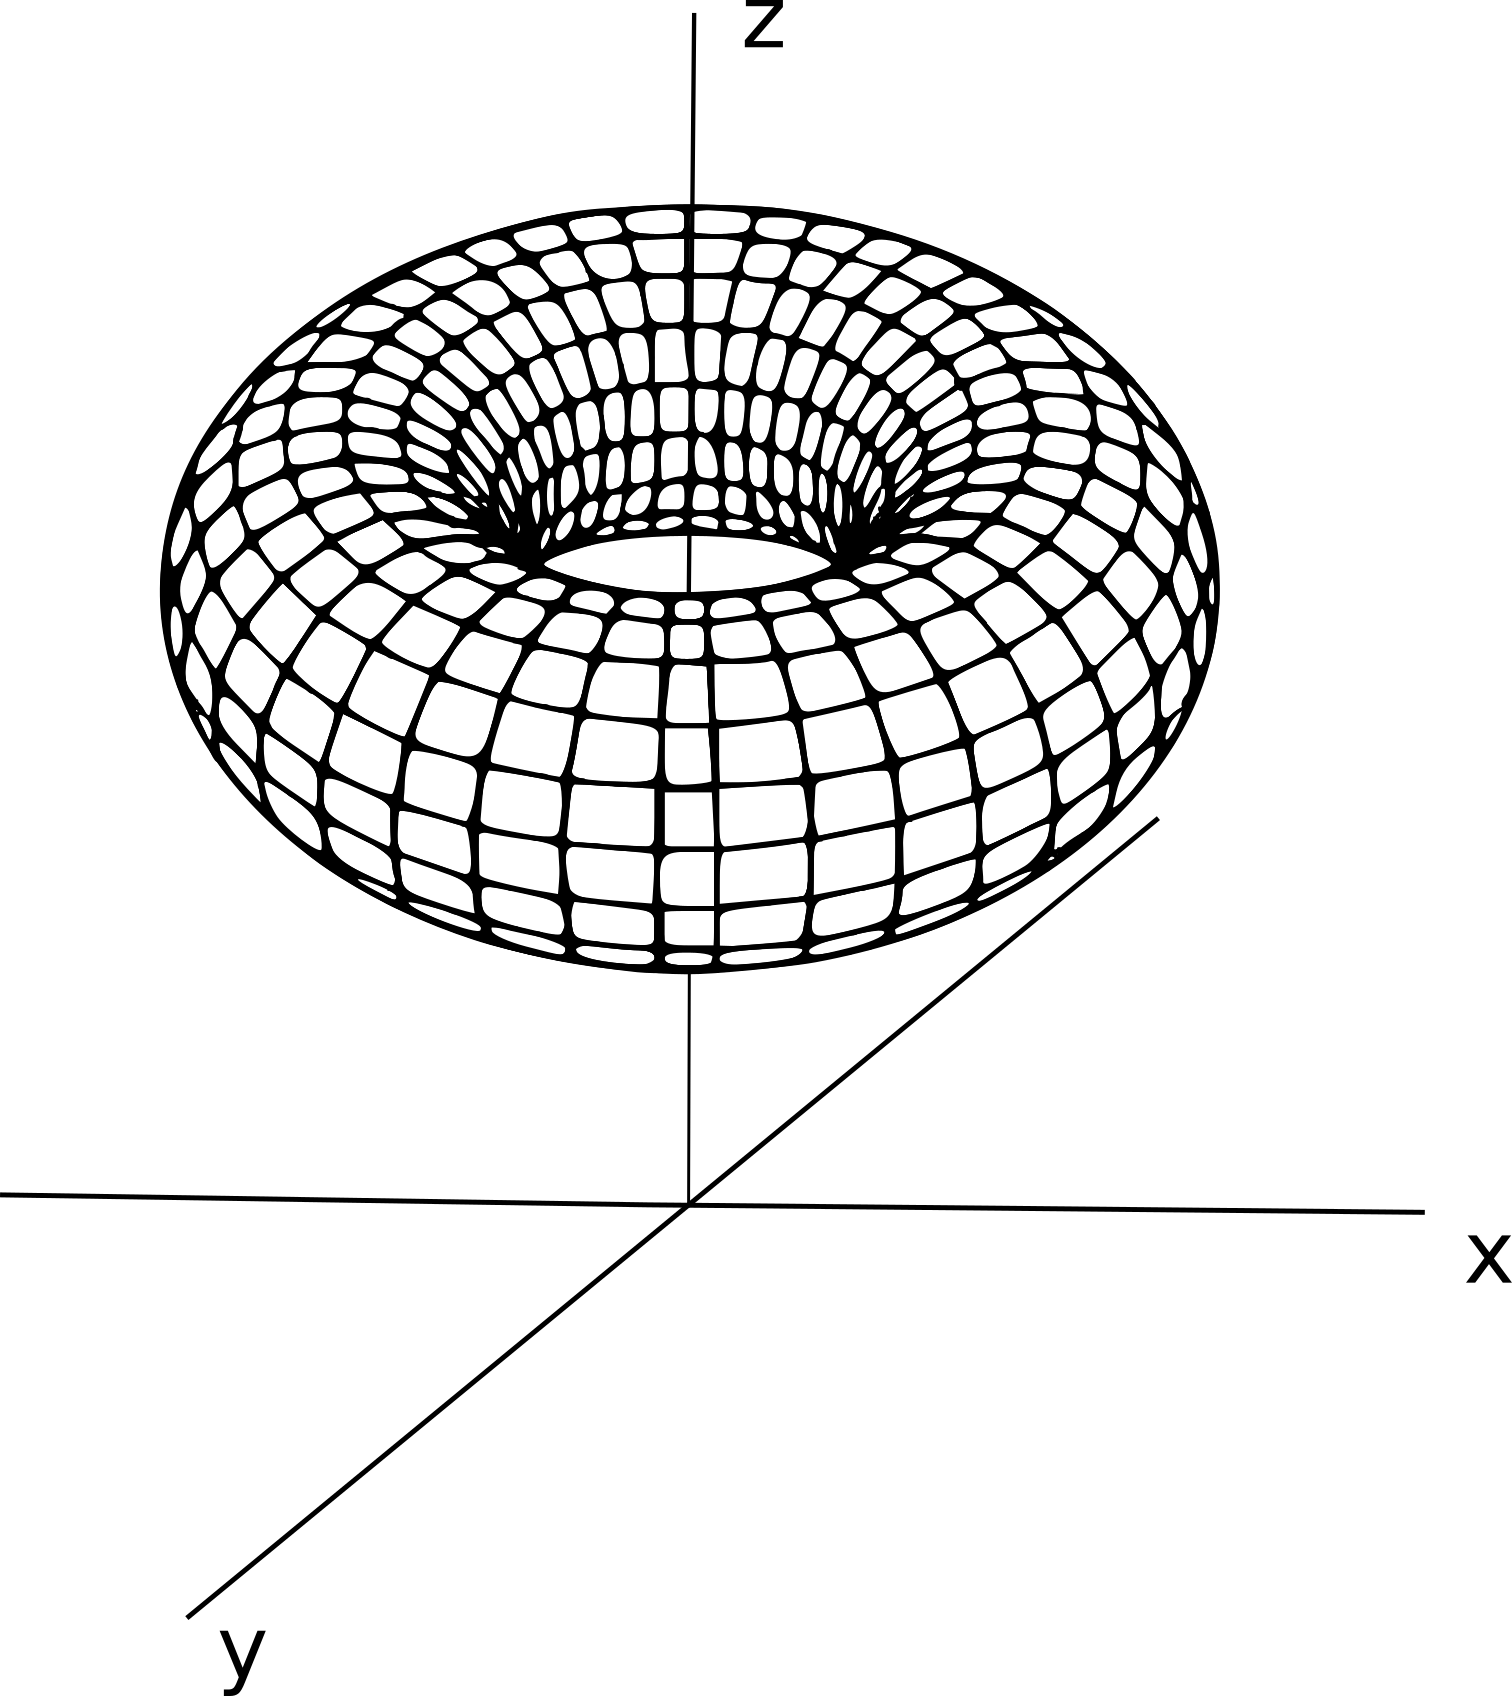
\includegraphics[scale=0.15]{Imagens/toro.png}
		\label{toro}
\end{figure}
\begin{figure}[H]
	\flushright
		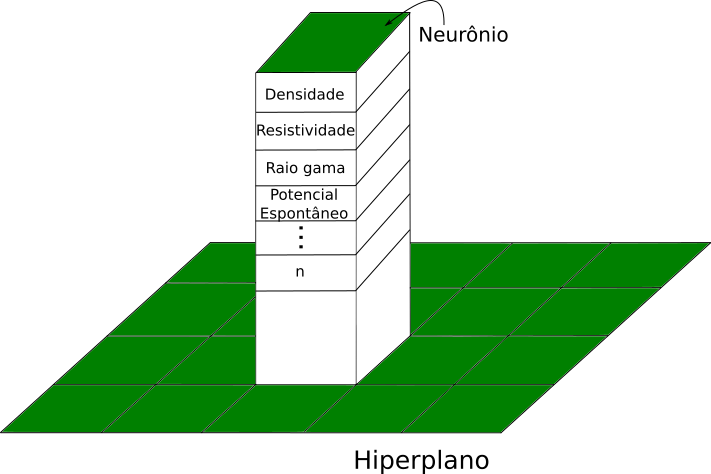
\includegraphics[scale=0.4]{Imagens/hiperplano.png}
	\label{hiperplano}
\end{figure}

\end{frame}

\begin{frame}
	\frametitle{Treinamento}

\begin{block}{Dado o vetor propriedades ...}
 \begin{displaymath}
 \mathbf{X}=\left(\begin{array}{r}
x_{1}\\
x_{2}\\
x_{3}\\
  \vdots \\
x_{m}
 \end{array}\right)
 \label{inicio}
 \end{displaymath}
\end{block}
\end{frame}

\begin{frame}
	\frametitle{Treinamento}
	\begin{block}{Cômputo da norma euclideana entre \textbf{X} e o  $w_{i,j}$}
		 \begin{eqnarray}
		 d(t)= \sqrt{\sum^{n}_{i=1}[x(t)-w_{i,j}(t)]^{2}} \hspace{1cm}  (j = {1,..,m}) 
		 \label{euclidiana}
		 \end{eqnarray}
		 Onde:
	\end{block}
	\begin{itemize}
		\pause
		\item $d(t)$, distância 
		\pause
		\item $x(t)$, vetor de propriedades
		\pause
		\item $w_{i,j}(t)$, matriz de pesos
	\end{itemize}
\end{frame}

\begin{frame}
	\frametitle{Treinamento}
	\begin{block}{Cálculo do neurônio vencedor}
	\begin{equation}
	w_{i,j}(t+1)=w_{i,j}(t)+\eta(t)[x(t)-w_{i,j}(t)] 
	\label{ajuste de pesos}
	\end{equation}
	\end{block}
		\begin{itemize}
			\pause
			\item $w_{i,j}(t+1)$, matriz de pesos atualizada
			\pause
			\item $\eta(t)$,  taxa de aprendizado
		\end{itemize}
\end{frame}


\begin{frame}
	\frametitle{Treinamento}
	\begin{block}{Aprendizado}
		\begin{equation}
		\eta(t)=\eta(0)    ( 1 -  \frac{t}{T}  )  
		\label{aprendizado}
		\end{equation}
	\end{block}
	\begin{itemize}
		\pause
		\item $T$, número de ciclos por treinamento,
		\pause
		\item $t$, número de iterações
		\pause
		\item ajusta-se $t=t+1$ e retorna para o início do processo até que $t=T$ \citep{YANG2009,Yan2014}.
	\end{itemize}
\end{frame}



\subsection{Treinamento não-supervisionado}

\begin{frame}
	\frametitle{Treinamento não-supervisionado}
	\begin{itemize}
		\item  Insere-se na rede os atributos de entrada;
		\pause
		\item Os valores de saída são definidos pela própria rede;
		\pause
		\item Indicado para os casos aonde se tem agrupamento de dados;
		\pause
		\item Inspira-se no funcionamento do córtex cerebal \citep{Schott1993}.
	\end{itemize}
	
		\begin{figure}[H]
			\centering
			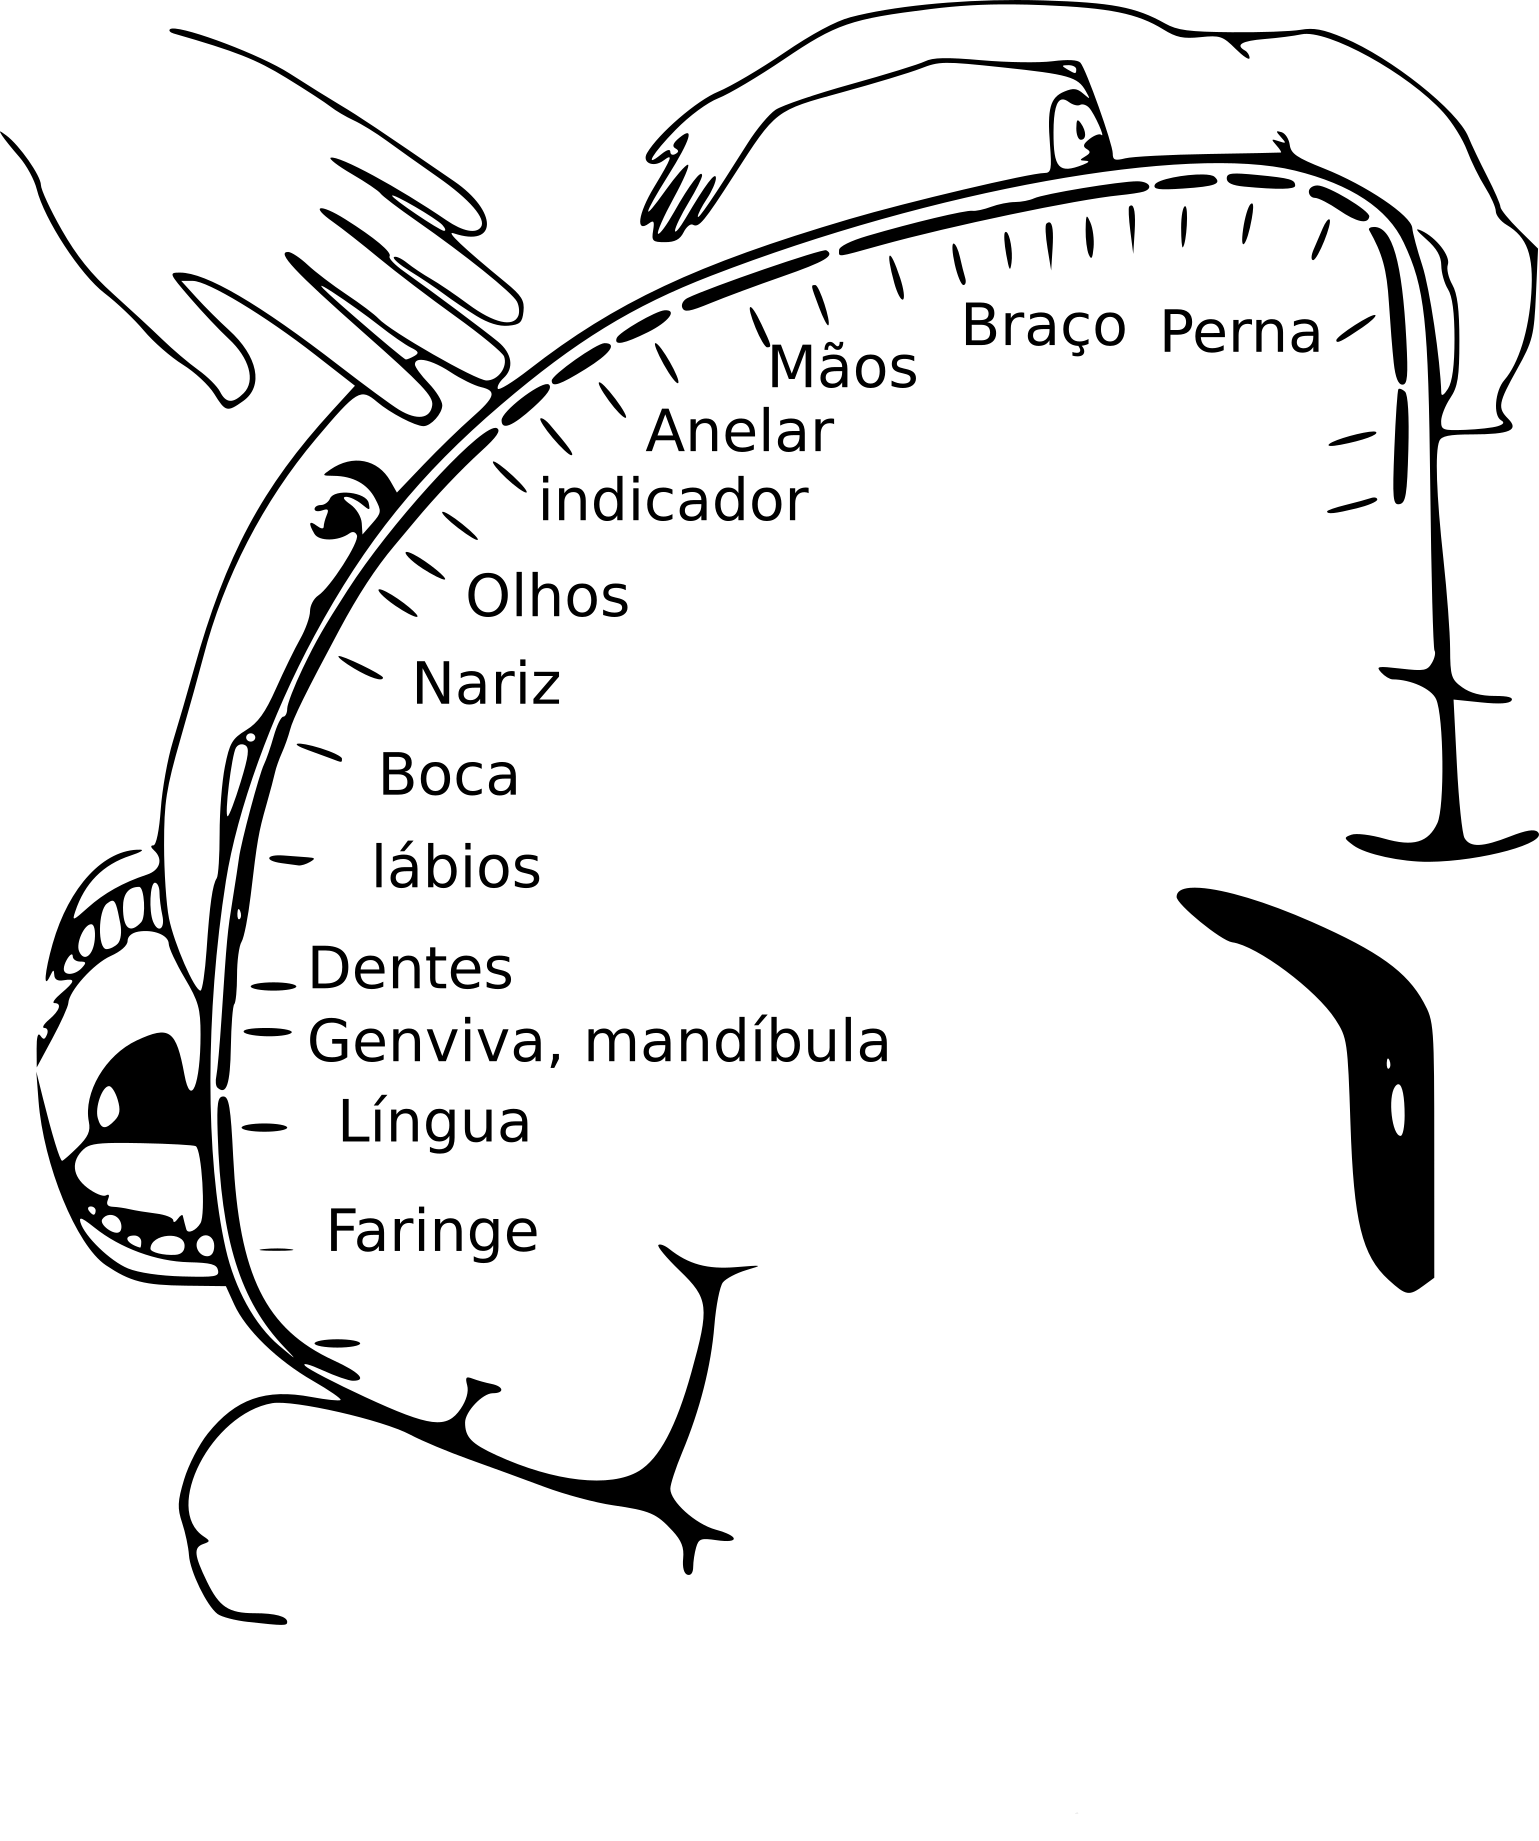
\includegraphics[scale=0.3]{Imagens/penfield.png}
			\caption{Homúnculo de Penfield }
			\label{penfield}
		\end{figure}
		
\end{frame}


%%%%%%%%%%%%%%%%%%%%%%%%%%%%%%%%%%%%%%%%%%%%%%%%%%%%%%%%%%%%%%%%%%%%%%%%%%%%
%---------------------------------CONTEXTO GEOLÓGICO------------------------------------
%%%%%%%%%%%%%%%%%%%%%%%%%%%%%%%%%%%%%%%%%%%%%%%%%%%%%%%%%%%%%%%%%%%%%%%%%%%%

\section{Contexto Geológico e Localização}
\begin{frame}[<+->]
	\frametitle{Contexto Geológico}
	\transboxin%efeito de transição	
	\begin{itemize}
		\justifying
		
		\item Localização: Centro-sul; 		
		\item Extensão: $1.100.000$ $Km^{2}$ \cite{Schneider_1974,zalan_p._v._tectonica_1987};
		\item Idade: Cambriano ao Quaternário com embasamento pré-cambriano\\ \cite{Schneider_1974,boletim_2007};
		\item Classificação: Bacia de sinéclise ou cratônica marginal, sob domínio flexural de crosta \cite{cordani_1984,borghi_2002}; 
		\item Depocentro: $7000$ m aproximadamente \cite{milani_outline_1999};
	\end{itemize}			
\end{frame}

%\begin{frame}
%	\frametitle{Contexto Geológico}
%	\transboxin%efeito de transição	
%	\begin{columns}
%		
%		\begin{column}{0.6\textwidth}
%			Três grupos de lineamentos: NW-SE (transamazônico), 
%			NE-SW (brasiliano) e
%			E-W (paralelos às fraturas de fundo oceânico)
%			\cite{zalan_p._v._tectonica_1987,milani_orogenias_1998,milani_outline_1999,borghi_2002}
%		\end{column}
%		
%		\begin{column}{0.4\textwidth}
%			\begin{figure}
%				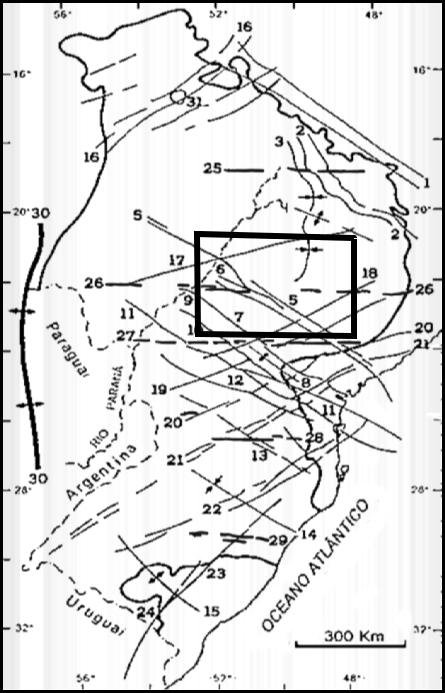
\includegraphics[scale=0.38]{Imagens/lineamentos.png}
%			\end{figure}
%		\end{column}
%	\end{columns}
%\end{frame}	

%%########## 2 ###########
%\begin{frame}
%	\frametitle{Contexto Geológico}
%	\begin{columns}
%		
%		\begin{column}{0.6\textwidth}
%			Três grupos de lineamentos: \textcolor{red}{NW-SE} (transamazônico), 
%			NE-SW (brasiliano) e
%			E-W (paralelos às fraturas de fundo oceânico)
%			\cite{zalan_p._v._tectonica_1987,milani_orogenias_1998,milani_outline_1999,borghi_2002}
%		\end{column}
%		
%		\begin{column}{0.4\textwidth}
%			\begin{figure}
%				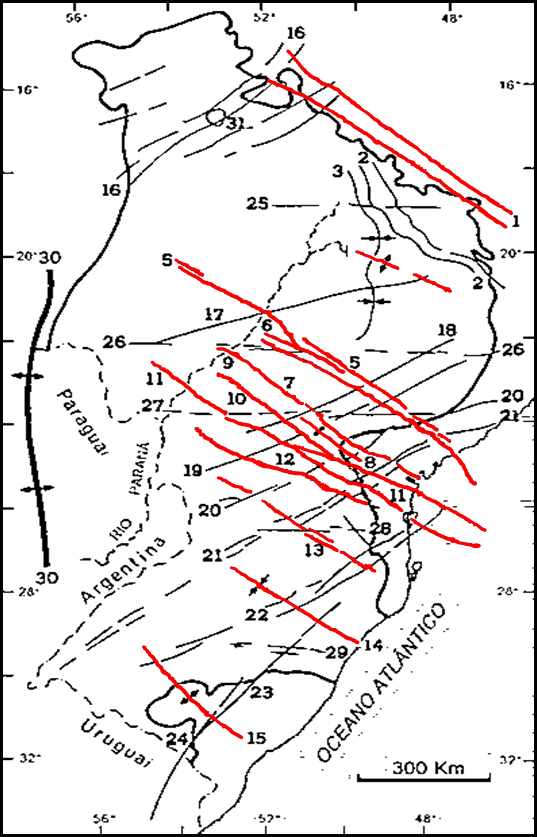
\includegraphics[scale=0.25]{Imagens/NW-SE.png}
%			\end{figure}
%		\end{column}
%	\end{columns}
%\end{frame}
%
%%########## 3 ###########
%\begin{frame}
%	\frametitle{Contexto Geológico}
%	\begin{columns}
%		
%		\begin{column}{0.6\textwidth}
%			Três grupos de lineamentos: NW-SE (transamazônico), 
%			\textcolor{green}{NE-SW} (brasiliano) e
%			E-W (paralelos às fraturas de fundo oceânico)
%			\cite{zalan_p._v._tectonica_1987,milani_orogenias_1998,milani_outline_1999,borghi_2002}
%		\end{column}
%		
%		\begin{column}{0.4\textwidth}
%			\begin{figure}
%				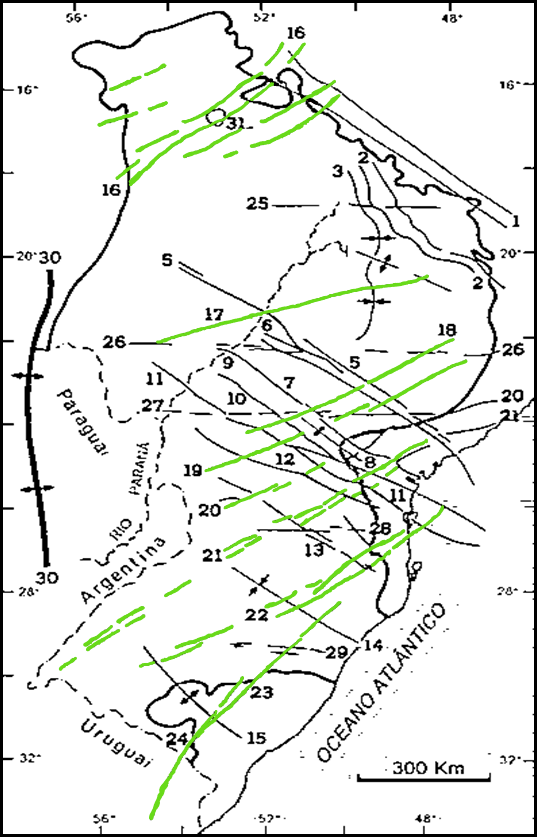
\includegraphics[scale=0.25]{Imagens/NE-SW.png}
%			\end{figure}
%		\end{column}
%	\end{columns}
%\end{frame}
%
%%########## 4 ###########
%\begin{frame}
%	\frametitle{Contexto Geológico}
%	\begin{columns}
%		
%		\begin{column}{0.6\textwidth}
%			Três grupos de lineamentos: NW-SE (transamazônico), 
%			NE-SW (brasiliano) e
%			\textcolor{blue}{E-W} (paralelos às fraturas de fundo oceânico)
%			\cite{zalan_p._v._tectonica_1987,milani_orogenias_1998,milani_outline_1999,borghi_2002}
%		\end{column}
%		
%		\begin{column}{0.4\textwidth}
%			\begin{figure}
%				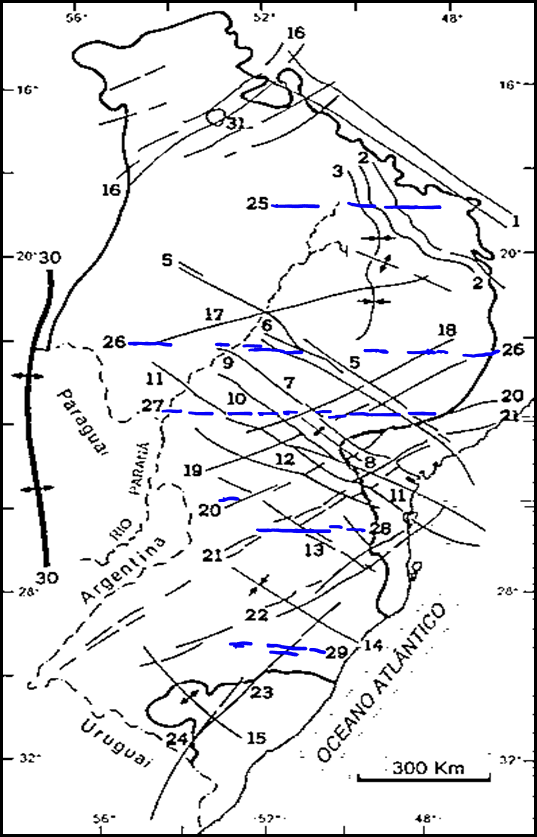
\includegraphics[scale=0.25]{Imagens/E-W.png}
%			\end{figure}
%		\end{column}
%	\end{columns}
%\end{frame}	
%
%%-------------------------------Estrutura do Embasamento-----------------------------------
%%########## 1 ###########
%%\begin{frame}
%%	\frametitle{Contexto Geológico}
%%	\begin{columns}
%%		
%%		\begin{column}{0.6\textwidth}
%%			Núcleos cratônicos associados às faixas móveis brasilianas, tais como o cráton do Guaxupé, Rio Paranapanema, Triângulo mineiro, Pelotas, Rio Apa e às faixas móveis Apiaí, Paraguai-araguaia, Uruaçu, Tijucas e Rio Paraná.
%%			\cite{Quintas_1995,Vidotti_1998,milani_orogenias_1998,hawkesworth_tectonic_2000,rosa_integracao_2009}
%%		\end{column}
%%		
%%		\begin{column}{0.4\textwidth}
%%			\begin{figure}
%%				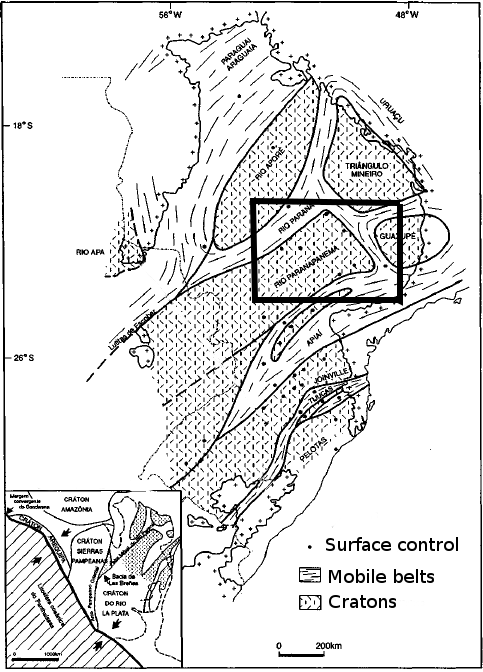
\includegraphics[scale=0.28]{Imagens/cratonsefaixasmoveis.png}
%%			\end{figure}
%%		\end{column}
%%	\end{columns}
%%\end{frame}
%
%%########## 2 ###########
%\begin{frame}
%	\frametitle{Contexto Geológico}
%	\begin{columns}
%		
%		\begin{column}{0.6\textwidth}
%			\textcolor{red}{Núcleos cratônicos} associados às faixas móveis brasilianas, tais como o cráton do \textcolor{red}{Guaxupé}, \textcolor{red}{Rio Paranapanema}, \textcolor{red}{Triângulo mineiro}, \textcolor{red}{Pelotas}, \textcolor{red}{Rio Apa} e às faixas móveis Apiaí, Paraguai-araguaia,  Uruaçu, Tijucas e Rio Paraná.
%			\cite{Quintas_1995,Vidotti_1998,milani_orogenias_1998,hawkesworth_tectonic_2000,rosa_integracao_2009}
%		\end{column}
%		
%		\begin{column}{0.4\textwidth}
%			\begin{figure}
%				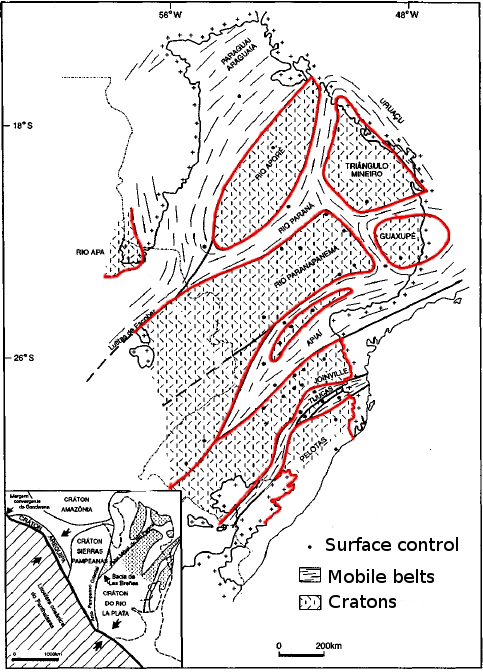
\includegraphics[scale=0.28]{Imagens/cratonsdestaque.png}
%			\end{figure}
%		\end{column}
%	\end{columns}
%\end{frame}	
%
%%########## 3 ###########
%\begin{frame}
%	\frametitle{Contexto Geológico}
%	\begin{columns}
%		
%		\begin{column}{0.6\textwidth}
%			Núcleos cratônicos associados às \textcolor{blue}{faixas móveis} brasilianas, tais como o cráton do Guaxupé, Rio Paranapanema, Triângulo mineiro, Pelotas, Rio Apa e às faixas móveis \textcolor{blue}{Apiaí}, \textcolor{blue}{Paraguai-araguaia}, \textcolor{blue}{Uruaçu}, \textcolor{blue}{Tijucas} e \textcolor{blue}{Rio Paraná}.
%			\cite{Quintas_1995,Vidotti_1998,milani_orogenias_1998,hawkesworth_tectonic_2000,rosa_integracao_2009}
%		\end{column}
%		
%		\begin{column}{0.4\textwidth}
%			\begin{figure}
%				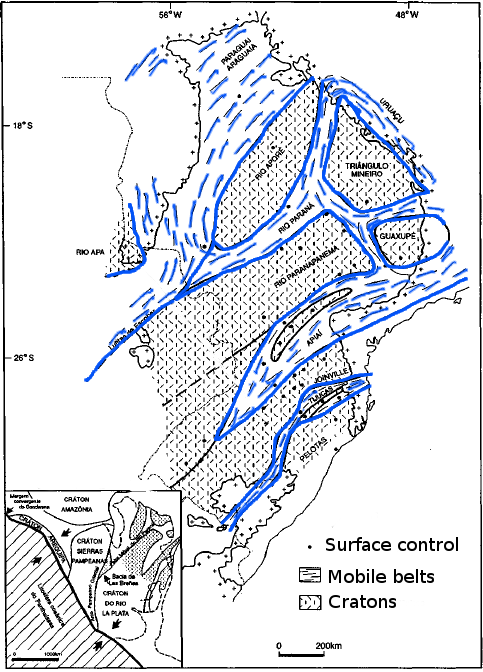
\includegraphics[scale=0.28]{Imagens/faixasmoveisdestaqueazul.png}
%			\end{figure}
%		\end{column}
%	\end{columns}
%\end{frame}	
%-----------------------------------Estratigrafia----------------------------------

%########## 1 ###########
\begin{frame}
	\frametitle{Contexto Geológico}
	\begin{columns}
		
		
		\begin{column}{0.4\textwidth}
			\begin{figure}
				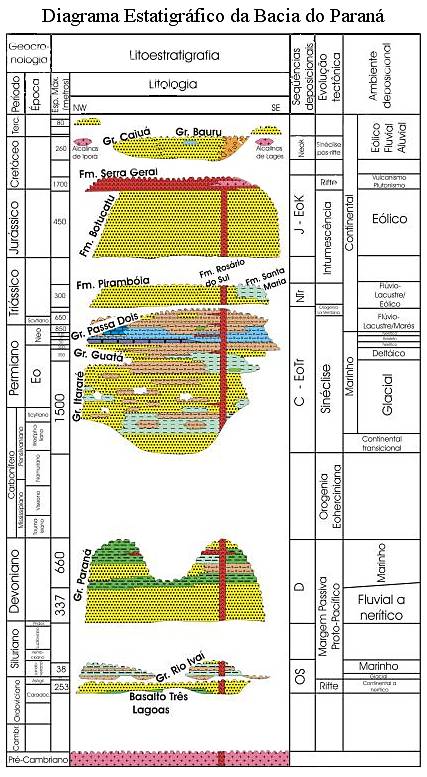
\includegraphics[scale=0.4]{Imagens/diagrama.png}
			\end{figure}
		\end{column}
		
		\begin{column}{0.75\textwidth}
			\begin{block}{As $6$ supersequências}
				Bauru $\Longleftrightarrow$  sequência neocretácea\\
				Gondwana III $\Longleftrightarrow$ sequência jurássica-eocretácea\\
				Gondwana II $\Longleftrightarrow$ sequência neotriássica \\
				Gondwana I $\Longleftrightarrow$ sequência carbonífera-permiana\\ 
				Paraná $\Longleftrightarrow$ sequência devoniana\\
				Rio Ivaí $\Longleftrightarrow$ sequência ordovício-siluriana\\
				\cite{Vail_1977,assine_1994,milani_orogenias_1998}
			\end{block}
			
		\end{column}
		
		
	\end{columns}
\end{frame}	

%########## 2 ###########
\begin{frame}
	\frametitle{Contexto Geológico}
	\begin{columns}
		\begin{column}{0.4\textwidth}
			\begin{figure}
				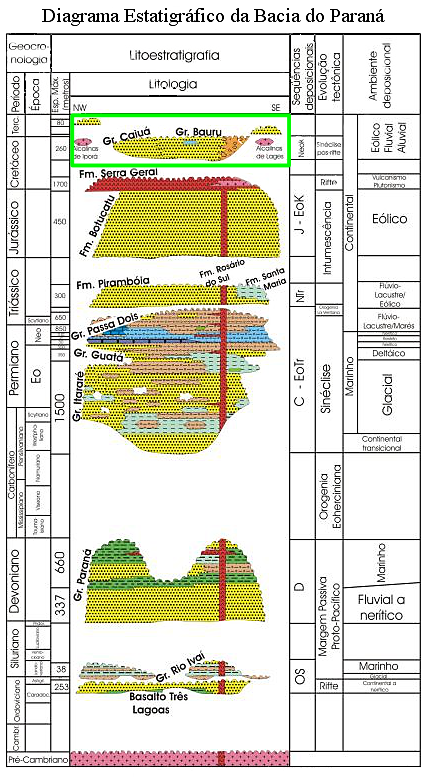
\includegraphics[scale=0.36]{Imagens/diagramabauru.png}
			\end{figure}
		\end{column}
		\begin{column}{0.75\textwidth}
			\begin{block}{As $6$ supersequências}
				\textcolor{green}{Bauru $\Longleftrightarrow$  sequência neocretácea}\\
				Gondwana III $\Longleftrightarrow$ sequência jurássica-eocretácea\\
				Gondwana II $\Longleftrightarrow$ sequência neotriássica \\
				Gondwana I $\Longleftrightarrow$ sequência carbonífera-permiana\\ 
				Paraná $\Longleftrightarrow$ sequência devoniana\\
				Rio Ivaí $\Longleftrightarrow$ sequência ordovício-siluriana\\
				\cite{Vail_1977,assine_1994,milani_orogenias_1998}
			\end{block}
		\end{column}
	\end{columns}
\end{frame}	

%########## 3 ###########
\begin{frame}
	\frametitle{Contexto Geológico}
	\begin{columns}
		\begin{column}{0.4\textwidth}
			\begin{figure}
				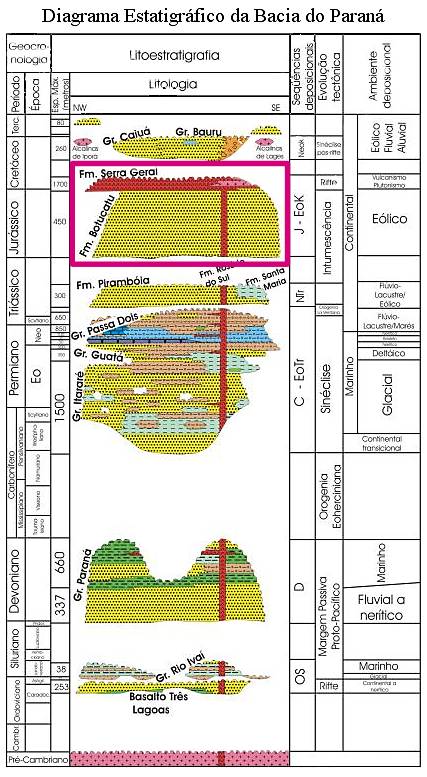
\includegraphics[scale=0.36]{Imagens/diagramagondwanaiii.png}
			\end{figure}
		\end{column}
		\begin{column}{0.75\textwidth}
			\begin{block}{As $6$ supersequências}
				Bauru $\Longleftrightarrow$  sequência neocretácea.\\
				\textcolor{purple}{Gondwana III $\Longleftrightarrow$ sequência jurássica-eocretácea}\\
				Gondwana II $\Longleftrightarrow$ sequência neotriássica \\
				Gondwana I $\Longleftrightarrow$ sequência carbonífera-permiana\\ 
				Paraná $\Longleftrightarrow$ sequência devoniana\\
				Rio Ivaí $\Longleftrightarrow$ sequência ordovício-siluriana\\
				\cite{Vail_1977,assine_1994,milani_orogenias_1998}
			\end{block}
		\end{column}
	\end{columns}
\end{frame}

%########## 4 ###########
\begin{frame}
	\frametitle{Contexto Geológico}
	\begin{columns}
		\begin{column}{0.4\textwidth}
			\begin{figure}
				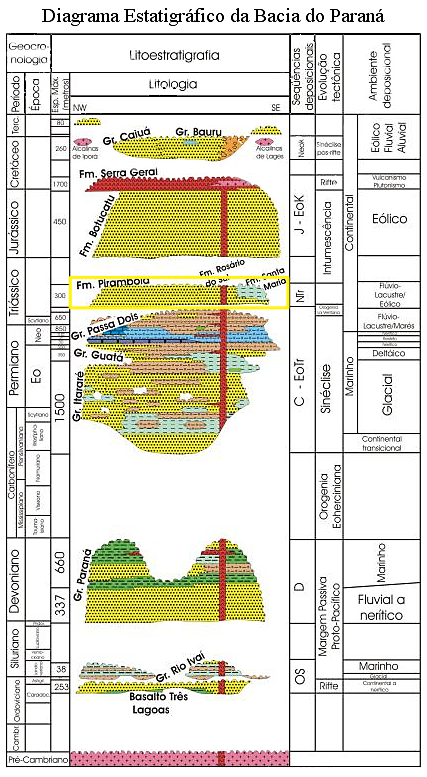
\includegraphics[scale=0.36]{Imagens/diagramagondwanaii.png}
			\end{figure}
		\end{column}
		\begin{column}{0.75\textwidth}
			\begin{block}{As $6$ supersequências}
				Bauru $\Longleftrightarrow$  sequência neocretácea.\\
				Gondwana III $\Longleftrightarrow$ sequência jurássica-eocretácea\\
				\textcolor{yellow}{Gondwana II $\Longleftrightarrow$ sequência neotriássica} \\
				Gondwana I $\Longleftrightarrow$ sequência carbonífera-permiana\\ 
				Paraná $\Longleftrightarrow$ sequência devoniana\\
				Rio Ivaí $\Longleftrightarrow$ sequência ordovício-siluriana\\
				\cite{Vail_1977,assine_1994,milani_orogenias_1998}
			\end{block}
		\end{column}
	\end{columns}
\end{frame}

%########## 5 ###########
\begin{frame}
	\frametitle{Contexto Geológico}
	\begin{columns}
		\begin{column}{0.4\textwidth}
			\begin{figure}
				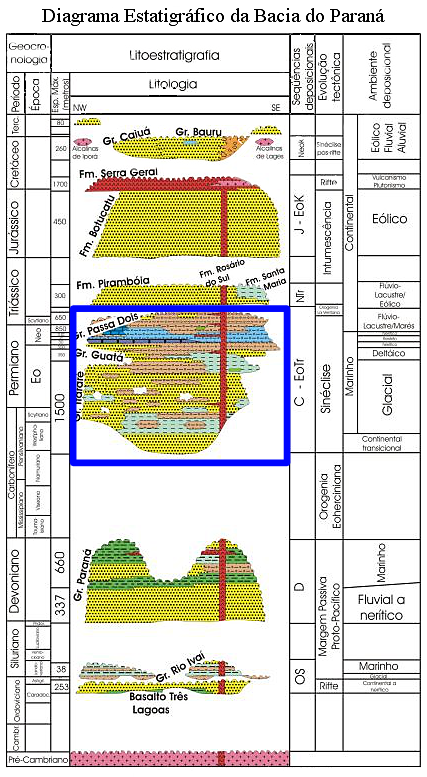
\includegraphics[scale=0.36]{Imagens/diagramagondwanai.png}
			\end{figure}
		\end{column}
		\begin{column}{0.75\textwidth}
			\begin{block}{As $6$ supersequências}
				Bauru $\Longleftrightarrow$  sequência neocretácea.\\
				Gondwana III $\Longleftrightarrow$ sequência jurássica-eocretácea\\
				Gondwana II $\Longleftrightarrow$ sequência neotriássica \\
				\textcolor{blue}{Gondwana I $\Longleftrightarrow$ sequência carbonífera-permiana}\\ 
				Paraná $\Longleftrightarrow$ sequência devoniana\\
				Rio Ivaí $\Longleftrightarrow$ sequência ordovício-siluriana\\
				\cite{Vail_1977,assine_1994,milani_orogenias_1998}
			\end{block}
		\end{column}
	\end{columns}
\end{frame}

%########## 6 ###########
\begin{frame}
	\frametitle{Contexto Geológico}
	\begin{columns}
		\begin{column}{0.4\textwidth}
			\begin{figure}
				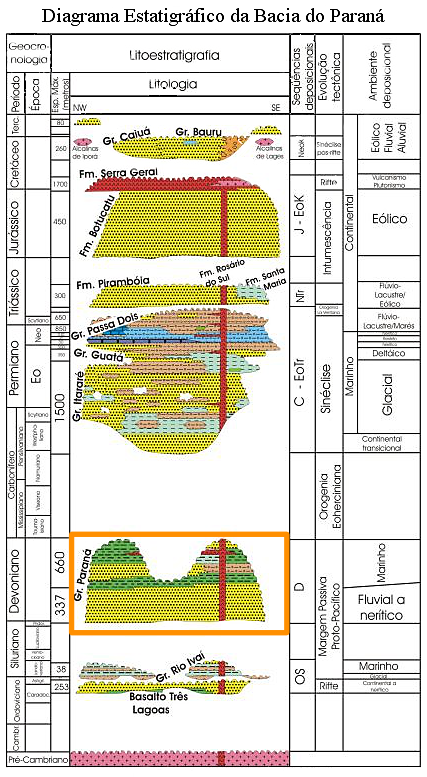
\includegraphics[scale=0.36]{Imagens/diagramaparana.png}
			\end{figure}
		\end{column}
		\begin{column}{0.75\textwidth}
			\begin{block}{As $6$ supersequências}
				Bauru $\Longleftrightarrow$  sequência neocretácea.\\
				Gondwana III $\Longleftrightarrow$ sequência jurássica-eocretácea\\
				Gondwana II $\Longleftrightarrow$ sequência neotriássica \\
				Gondwana I $\Longleftrightarrow$ sequência carbonífera-permiana\\ 
				\textcolor{orange}{Paraná $\Longleftrightarrow$ sequência devoniana}\\
				Rio Ivaí $\Longleftrightarrow$ sequência ordovício-siluriana\\
				\cite{Vail_1977,assine_1994,milani_orogenias_1998}
			\end{block}
		\end{column}
	\end{columns}
\end{frame}

%########## 7 ###########
\begin{frame}
	\frametitle{Contexto Geológico}
	\begin{columns}
		\begin{column}{0.4\textwidth}
			\begin{figure}
				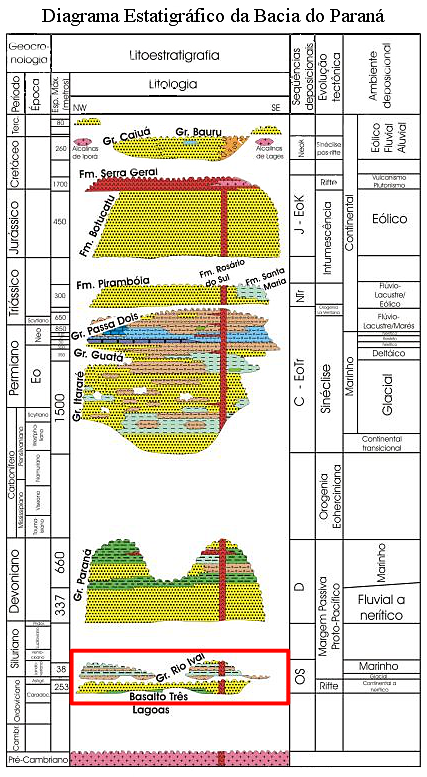
\includegraphics[scale=0.36]{Imagens/diagramarioivai.png}
			\end{figure}
		\end{column}
		\begin{column}{0.75\textwidth}
			\begin{block}{As $6$ supersequências}
				Bauru $\Longleftrightarrow$  sequência neocretácea.\\
				Gondwana III $\Longleftrightarrow$ sequência jurássica-eocretácea\\
				Gondwana II $\Longleftrightarrow$ sequência neotriássica \\
				Gondwana I $\Longleftrightarrow$ sequência carbonífera-permiana\\ 
				Paraná $\Longleftrightarrow$ sequência devoniana\\
				\textcolor{red}{Rio Ivaí $\Longleftrightarrow$ sequência ordovício-siluriana}\\
				\cite{Vail_1977,assine_1994,milani_orogenias_1998}
			\end{block}
		\end{column}
	\end{columns}
\end{frame}


\begin{frame}
	\frametitle{Localização e extensão da Bacia Sedimentar}
	\begin{figure}[H]
		\centering
			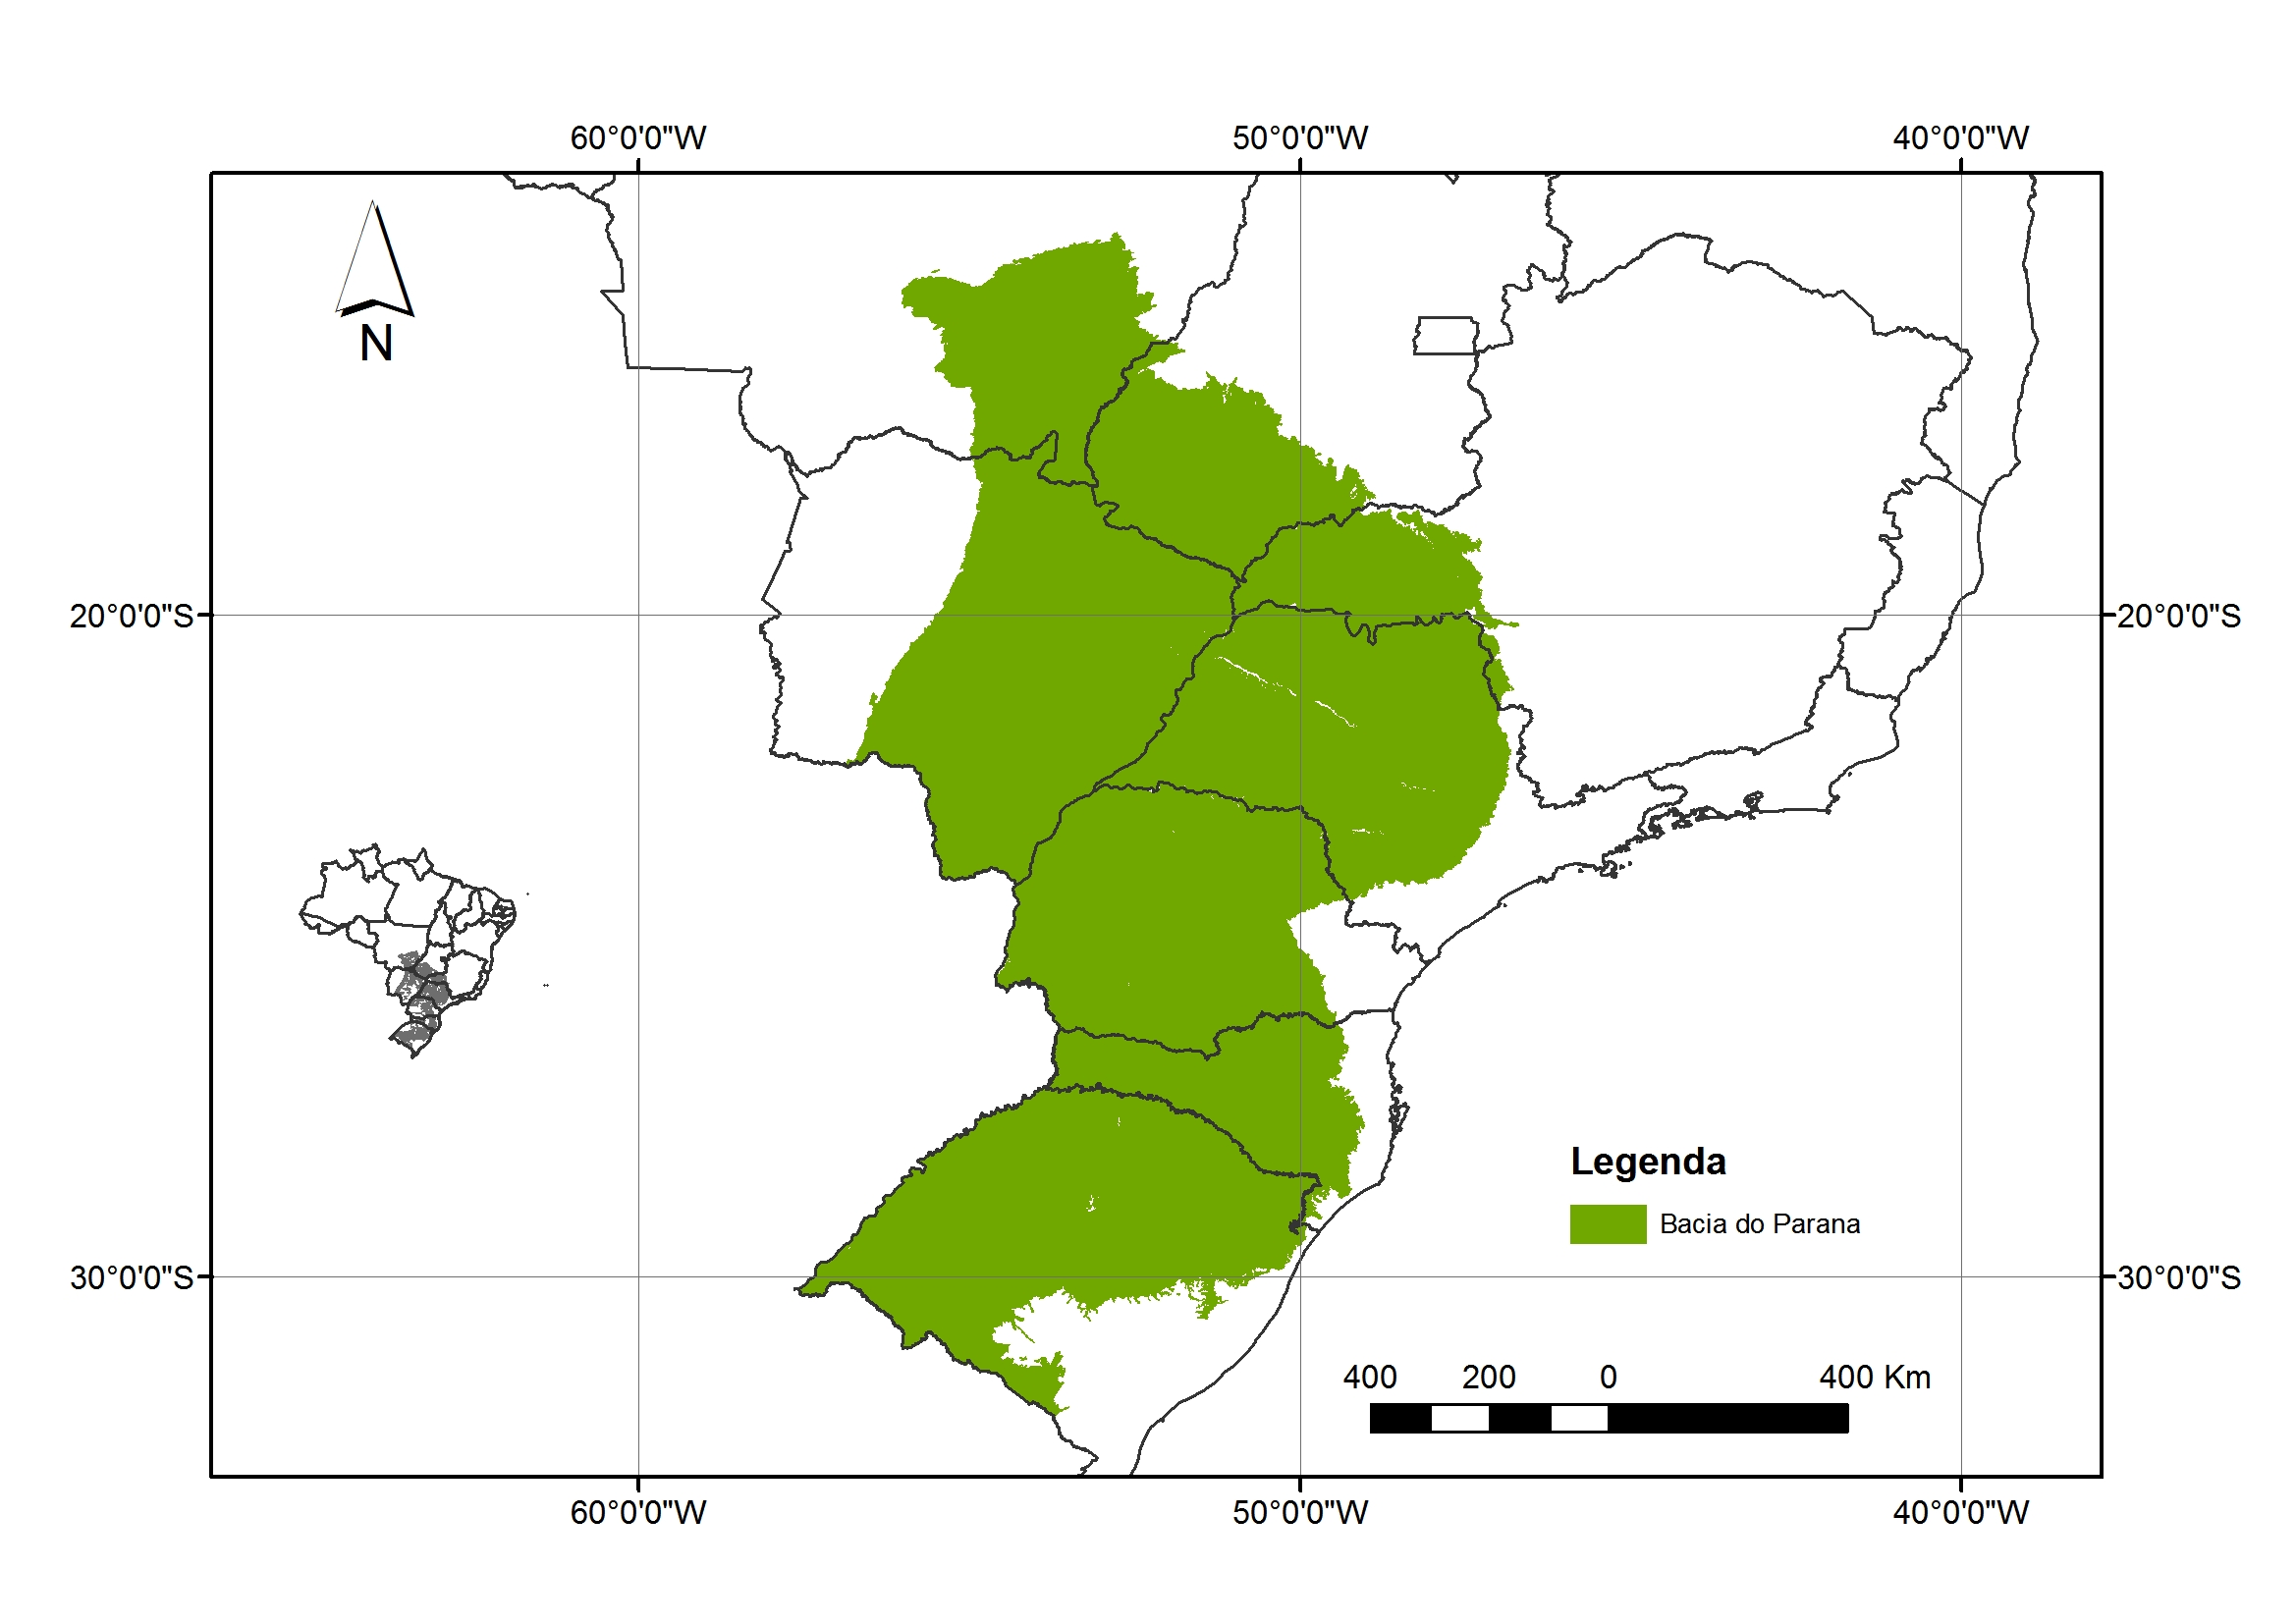
\includegraphics[scale=0.3]{Imagens/BaciaParana.jpg}
		\caption{Mapa de localização da Bacia do Paraná. }
		\label{mapa geologico}
	\end{figure}
\end{frame}

\begin{frame}
	\frametitle{Localização dos poços}
	\begin{figure}[H]
		\centering
		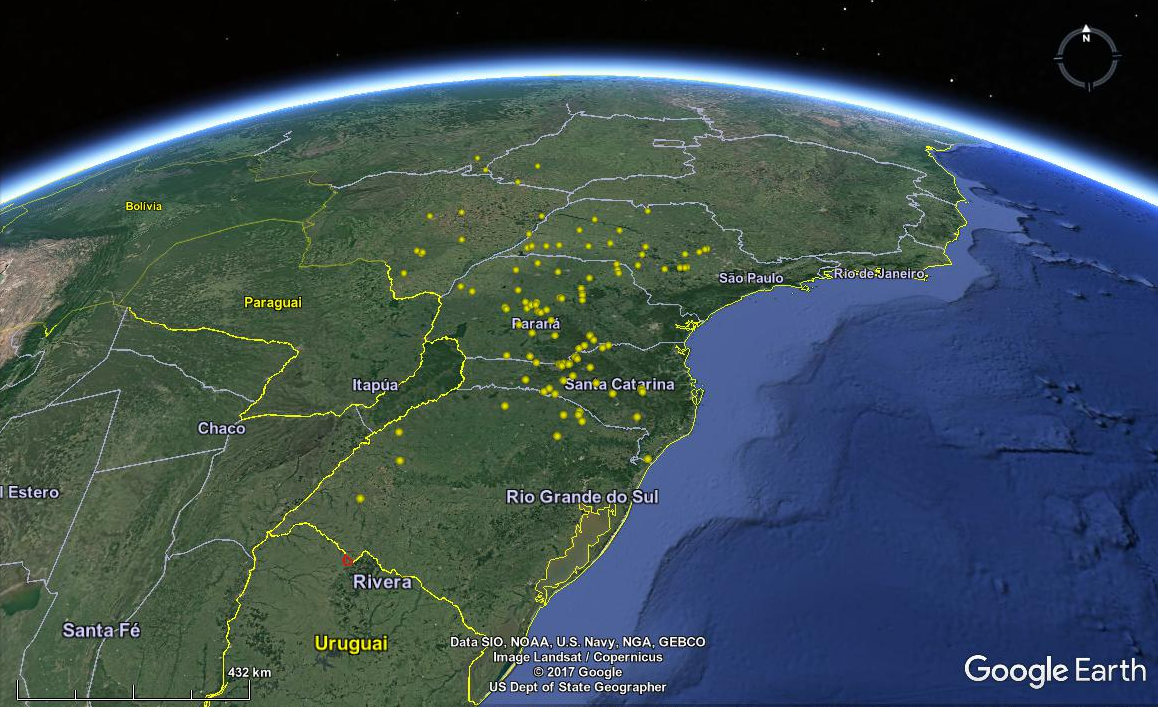
\includegraphics[scale=0.25]{Imagens/Pocos2.png}
		\caption{Localização dos poços de trabalho.}
		\label{real}
	\end{figure}
\end{frame}

\begin{frame}
	\frametitle{Dado}
	\begin{figure}[H]
		\centering
		\includegraphics[scale=0.12]{Imagens/poco.png}
		\caption{Dado de perfilagem }
	\end{figure}
\end{frame}

%%%%%%%%%%%%%%%%%%%%%%%%%%%%%%%%%%%%%%%%%%%%%%%%%%%%%%%%%%%%%%%%%%%%%%%%%%%%
%-------------------------OBJETIVO------------------------------
%%%%%%%%%%%%%%%%%%%%%%%%%%%%%%%%%%%%%%%%%%%%%%%%%%%%%%%%%%%%%%%%%%%%%%%%%%%%
\section{Objetivo}

\begin{frame}
	\frametitle{Objetivo}
	\begin{itemize}
		\item Desenvolver uma rede neuronal artificial otimizada que classifique tipos litológicos distintos;
		\pause
		\item  Aplicar a rede na identificação de rochas da Bacia do Paraná. 
	\end{itemize}
\end{frame}


\section{Metodologia}

\subsection{Dados Sintéticos}
\begin{frame}
	\frametitle{Fluxograma de criação dos dados sintéticos}
\begin{footnotesize}
	\begin{figure}[H]
		\centering

		\begin{tikzpicture}
		[node distance=.5cm,
		start chain=going below,]
		\node[punktchain, join]  {Modelo de Bacia};
		\node[punktchain, join]   {Dados da Literatura};
		\node[punktchain, join]   {Estimar erros das propriedades físicas para dada litologia};
		\node[punktchain, join] {Definir taxa de amostragem};
		\node[punktchain, join, ] {Gerar dados sintéticos contaminados com o erro gaussiano estimado};
		
		\end{tikzpicture}
%		\caption{Fluxograma do programa de geração dos dados sintéticos}
	\end{figure}
	
\end{footnotesize}	
\end{frame}

\subsection{Treinamento da rede}
\begin{frame}
	\frametitle{Fluxograma de treinamento}
	\begin{scriptsize}
		

	\begin{figure}[H]
		\centering
	
%		\begin{tikzpicture}
%		[node distance=.3cm,
%		start chain=going below,]
%		\node[punktchain, join]  {Início};
%		\node[punktchain, join] (L1)  {Entrar com os dados do treinamento};
%		\node[punktchain, join]   {Atualizar o peso do neurônio vencedor};
%		\node[punktchain, join] (L2) {Fazer alteração nas vizinhanças do neurônio vencedor. Varre os dados de forma sequencial};
%		\node[punktchain, join, ] {Avaliar o nível de treinamento da rede};
%		\node[punktchain, join, ] {\color{red}Caso não esteja satisfatório volta-se para o Início e repete o processo de forma acumulativa};
%		\node[punktchain, join, ] {\color{blue}Caso esteja satisfatório é o decretado o final do treinamento};	
%		\end{tikzpicture}
			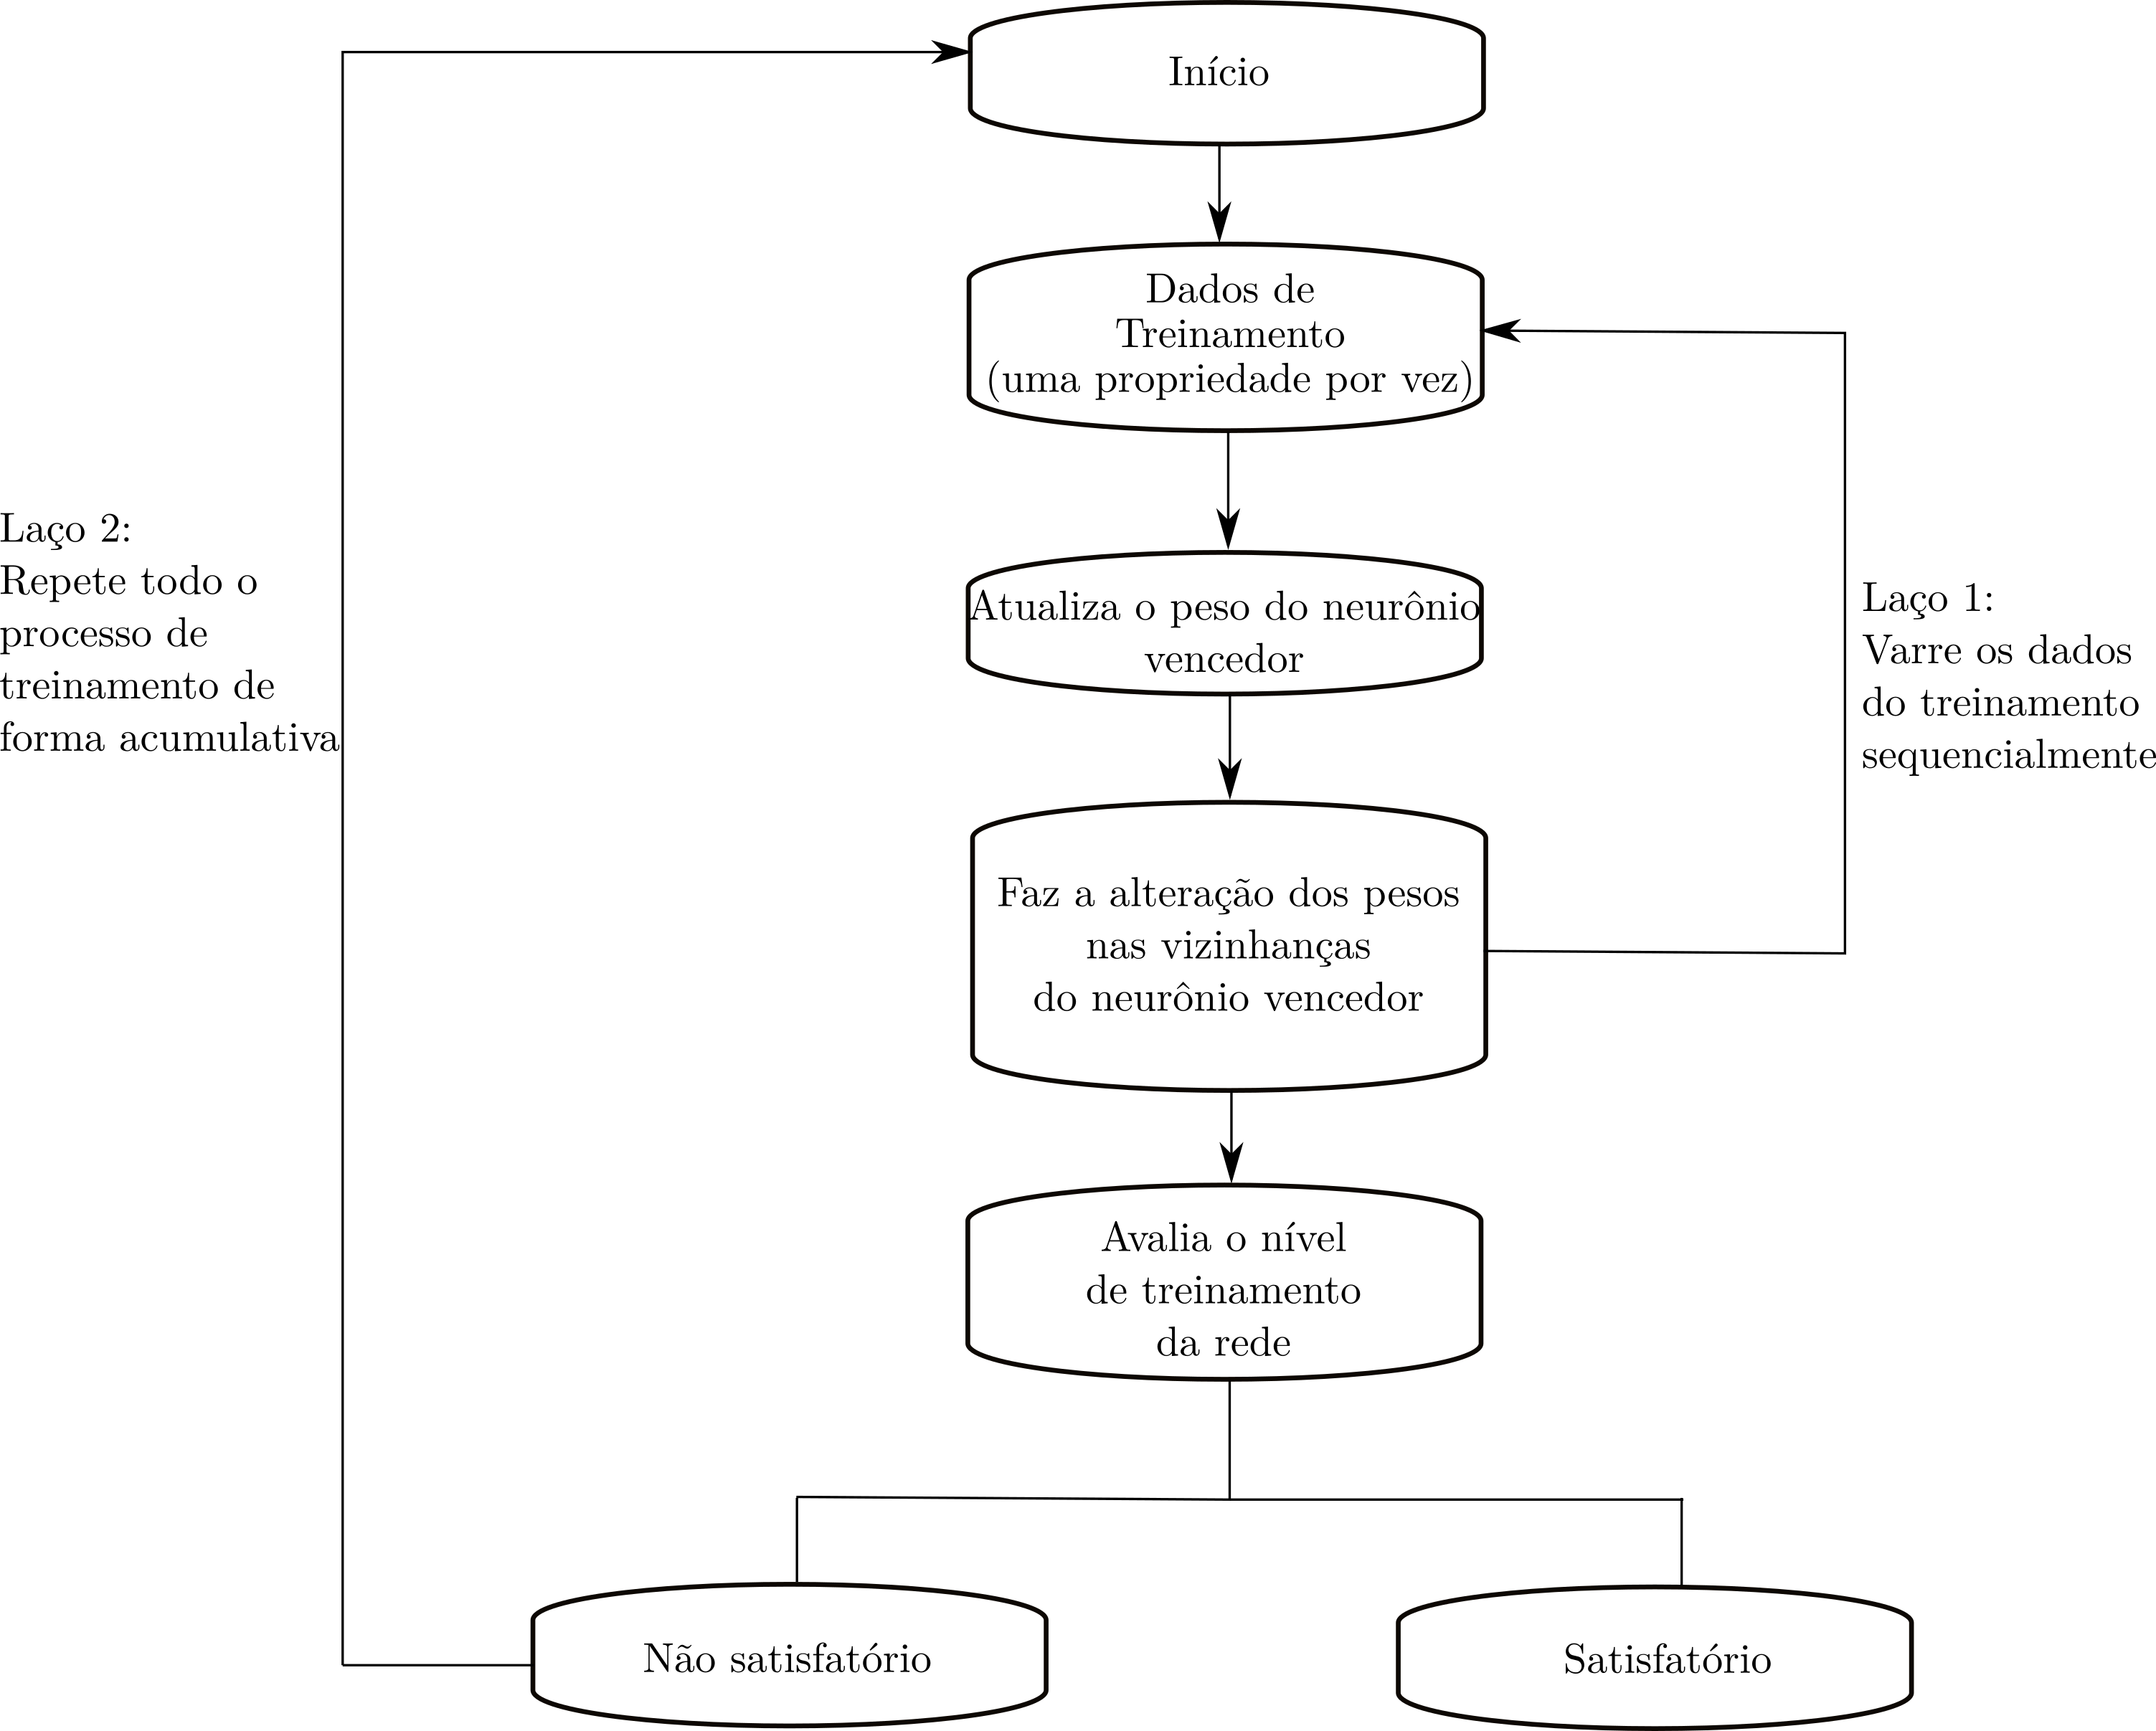
\includegraphics[scale=0.4]{Imagens/treinamento.png}
	\end{figure}
\end{scriptsize}
\end{frame}


\subsection{Classificação da rede}
\begin{frame}
	\frametitle{Fluxograma de classificação}
	\begin{small}
		
		
		\begin{figure}[H]
			\centering
			
%	\begin{tikzpicture}
%	[node distance=.8cm,
%	start chain=going below,]
%	\node[punktchain, join]  {Entrada do dado não classificado};
%	\node[punktchain, join] (L1)  {Determinação da distância entre os dados de cada neurônio };
%	\node[punktchain, join]   {Armazena as distâncias};
%	\node[punktchain, join] (L2) {Seleciona a menor distância};
%	\node[punktchain, join, ] {Classifica o dado};	
%	\end{tikzpicture}
	
		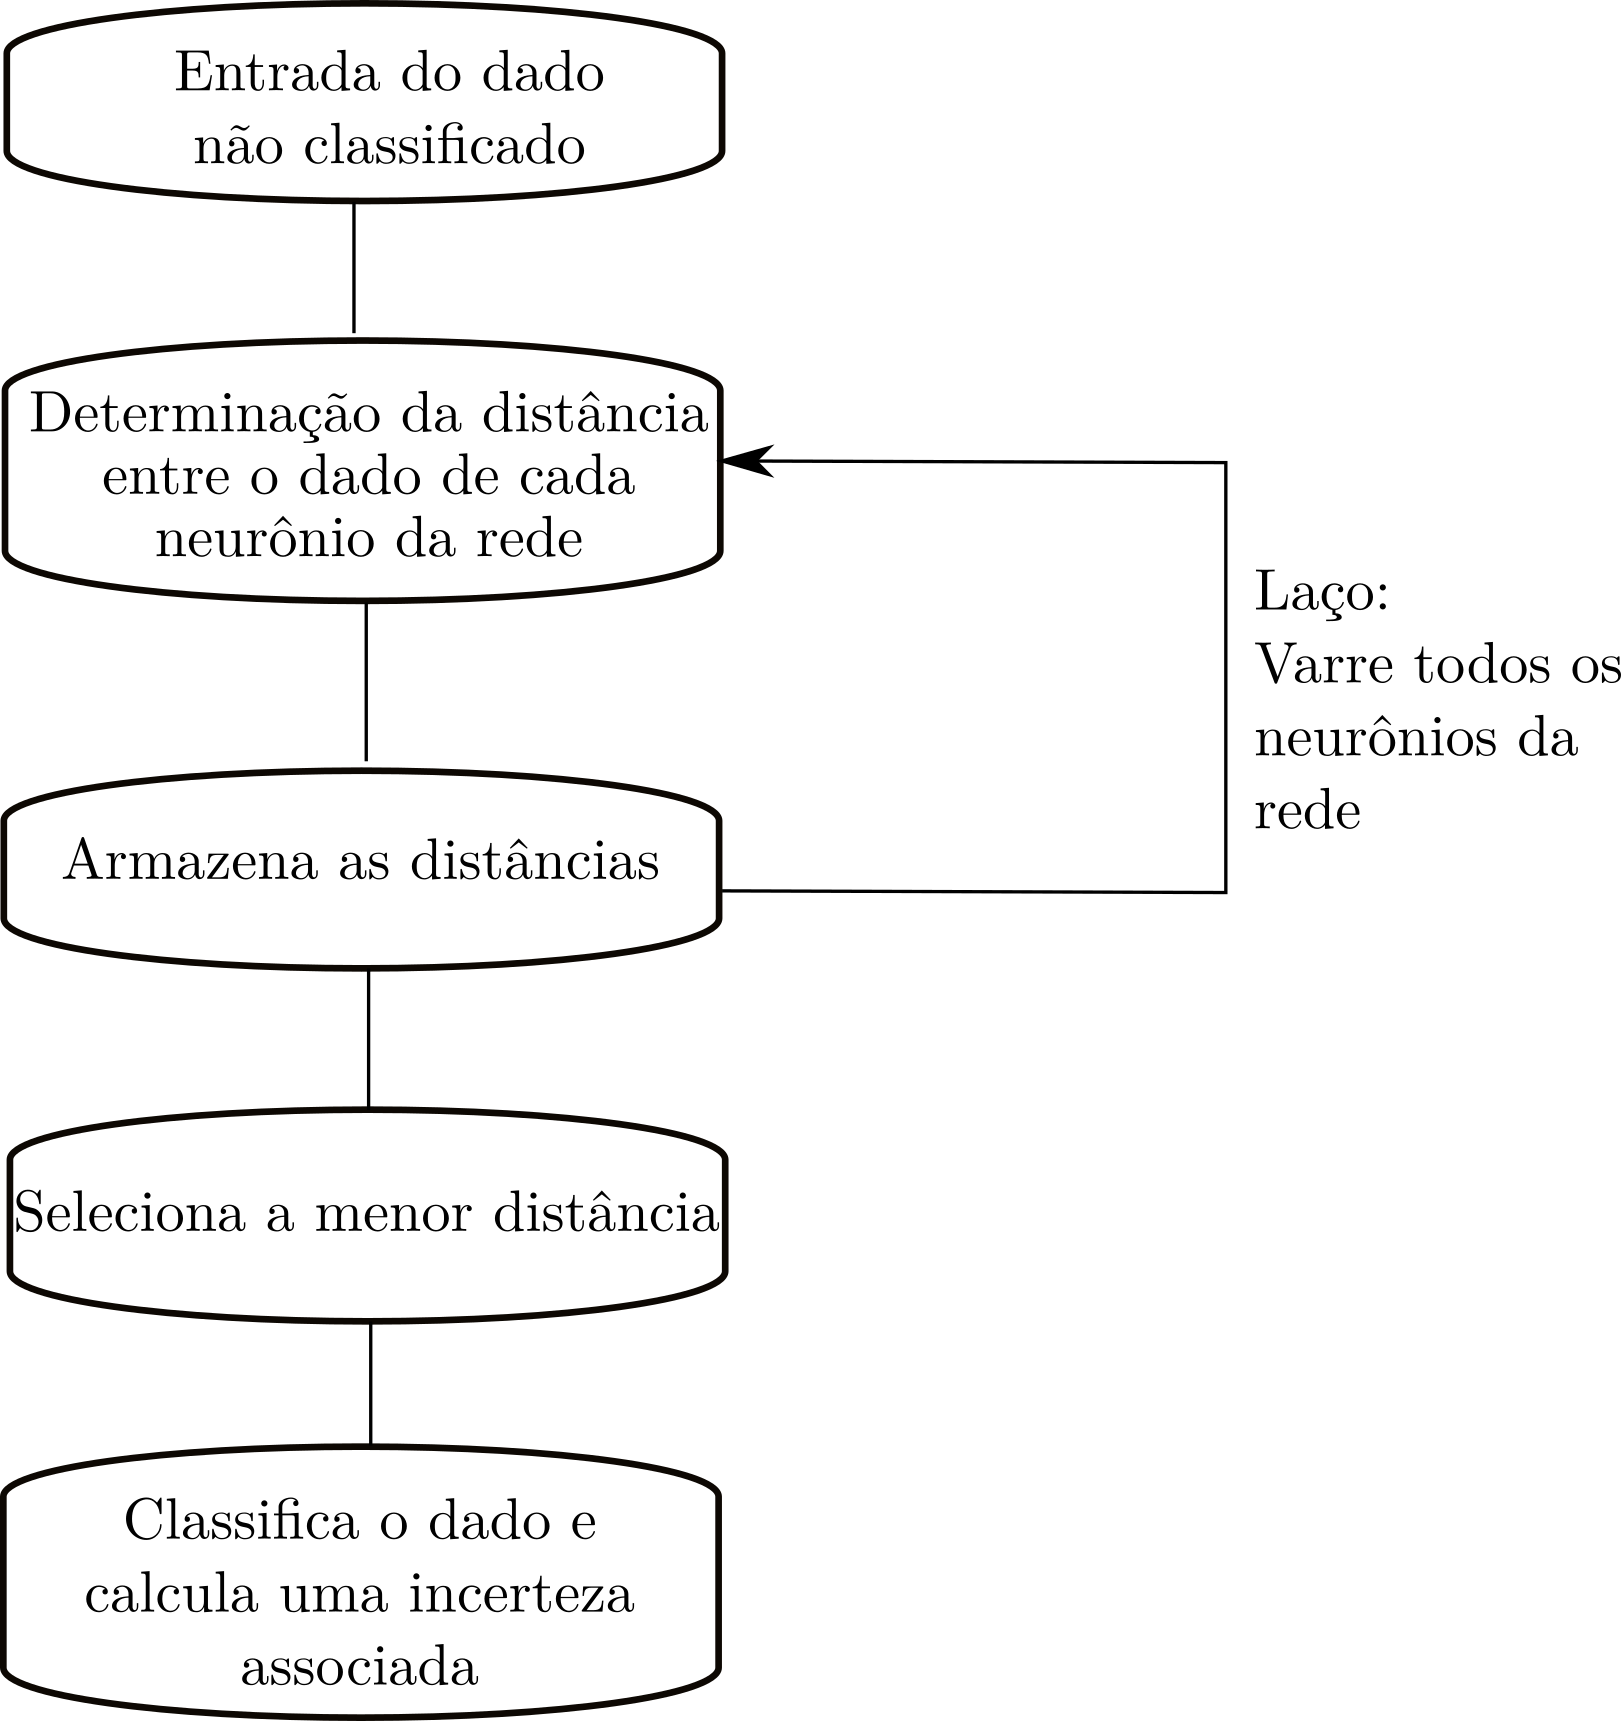
\includegraphics[scale=0.55]{Imagens/classificacao.png}
		\end{figure}
	\end{small}
\end{frame}







%%%%%%%%%%%%%%%%%%%%%%%%%%%%%%%%%%%%%%%%%%%%%%%%%%%%%%%%%%%%%%%%%%%%%%%%%%%%
%---------------------------NATUREZA DO DADO--------------------------
%%%%%%%%%%%%%%%%%%%%%%%%%%%%%%%%%%%%%%%%%%%%%%%%%%%%%%%%%%%%%%%%%%%%%%%%%%%%

\section{Modelo proposto}

\begin{frame}
	\frametitle{Modelo proposto}
 \begin{scriptsize}
	\begin{table}[H]
		\centering
		\caption{Compilação de propriedades físicas usadas para inferência de litologia \citep{Telford_1993}.}
		\label{rock-properties1}
			\begin{tabular}{@{}llllllllll@{}}
				\toprule
				Rocha         & Densidade ($g/cm^{3}$) & Raios-Gama ($Ci/g$)& Potencial-Espontâneo ($mV$)&   \\ \midrule
				Conglomerado &     $2,50$  &       ---        &    ---        &      \\
				Arenito  &    $2,35$      &       $2,00\leftrightarrow4,00$       &     ---       &      \\
				Folhelho &   $2,40$       &      ---        &      ---      &    \\
				Argilito &     $2,55$   &          ---     &       ---     &     \\
				Siltito  &      $2,21$    &          ---     &       ---     &   \\
				Dolomita &     $2,70$    &        $8,00$       &   ---         &       \\
				Marga  &    $2,50$     &         ---      &    ---        &     \\
				Basalto  &     $2,99$    &          $0,50$     &    ---       &      \\
				Diabásio &    $2,90$    &         ---      &       ---     &     \\
				Lava &     $2,61$    &      $0,33$         &      ---      &      \\
				Granito &    $2,64$      &       $0,70\leftrightarrow4,80$        &      ---      &      \\
				Gabro &    $3,03$     &       ---        &     ---       &       \\
				Peridotito &   $3,15$    &      ---         &     ---       &      \\
				Quartzito &    $2,60$    &        $5,00$      &     ---       &    \\
				Xisto &   $2,64$    &         ---      &      ---      &    \\
				Gnaisse &    $2,80$     &      ---         &    ---        &        \\
				Serpentinito &    $2,78$     &   ---            &   ---     &        \\
				Anfibolito &  $2,96$       &          ---     &       ---     &        \\
				Eclogito &  $3,37$    &       ---        &      ---      &    \\
				Mármore &   $2,75$       &      ---         &     ---       &      \\ \bottomrule
			\end{tabular}
	\end{table}
\end{scriptsize}
\end{frame}

\begin{frame}
	\frametitle{Modelo proposto}
	\begin{scriptsize}
		\begin{table}[H]
			\centering
			\caption{Compilação de propriedades físcas usadas na inferência de porosidade, permeabilidade. \cite{Telford_1993}.}
			\label{rock-properties2}
			\begin{tabular}{@{}llllllllll@{}}
				\toprule
				Rocha   & Resistividade ($\Omega/m$) &  Neutrão ($API$) & Velocidade ($km/s$)  &    \\ \midrule
				Conglomerado &    $2\times10^{3}\leftrightarrow10^{4}$       &    ---           &     $1,80\leftrightarrow4,90$       &     \\
				Arenito  &    $1\leftrightarrow6,4\times10^{8}$       &      ---         &     $4,00\leftrightarrow4,30$       &   \\
				Folhelho &     $50\leftrightarrow10^{7}$      &      ---         &      $2,15\leftrightarrow3,30$      &   \\
				Argilito &     $10\leftrightarrow8\times10^{2}$      &       ---        &     ---       &      \\
				Siltito  &      $1\leftrightarrow100$     &      ---         &         $4,00\leftrightarrow6,20$    &         \\
				Dolomita &   $3,5\times10^{2}\leftrightarrow5\times10^{3}$        &    ---           &      $5,70\leftrightarrow6,00$      &      \\
				Marga  &     $3\leftrightarrow70$      &     ---          &     ---       &     \\
				Basalto  &     $10\leftrightarrow1,3\times10^{7}$      &     ---          &     $ 5,00\leftrightarrow5.80$         &     \\
				Diabásio &  $20\leftrightarrow5\times10^{7}$         &      ---         &     ---       &  \\
				Granito Porfirítico (seco) &     $1,3\times10^{6}$     &       ---        &     $5,80$       &    \\
				Granito Porfirítico (úmido) &  $4,5\times10^{3}$          &      ---         &     $ 5,00\leftrightarrow5.60$         &      \\
				Gabro &   $10^{3}\leftrightarrow10^{6}$       &      ---         &      $ 5,00\leftrightarrow5.80$        &     \\
				Peridotito (seco) &   $6,5\times10^{3}$        &    ---           &       ---     &    \\
				Peridotito (úmido) &    $3\times10^{3}$       &      ---         &      ---      &  \\
				Xisto &    $20\leftrightarrow10^{4}$       &        ---       &       ---     &   \\
				Gnaisse (seco) & $3\times10^{6}$          &         ---      &     ---       &   \\
				Gnaisse (úmido) &   $6,8\times10^{4}$        &       ---        &      ---      &   \\
				Tufa (seca) &      $2\times10^{3}$     &      ---         &     $1,80\leftrightarrow3,50$       &     \\
				Tufa (úmida) &     $10^{5}$      &     ---          &     ---       &      \\
				Mármore &  $10^{2}\leftrightarrow2,5\times10^{8}$         &       ---        &      ---      &    \\ \bottomrule
			\end{tabular}
		\end{table}
	\end{scriptsize}
\end{frame}

\begin{frame}
	\frametitle{Parâmetros do modelo}
	\begin{scriptsize}
		\begin{table}[H]
			\centering
			\label{parametros}
			\begin{tabular}{@{}ccccccccccc@{}}
				\toprule
				Rocha        & Densidade ($g/cm^{3}$) & Raios-Gama ($Ci/g$) & Resistividade ($\Omega/m$)&  Velocidade ($Km/s$) &\\ \midrule
				Conglomerado &       $2,30$ 		  &       $100,0$       &           $6000$           &			$2$   		   	&\\
				Folhelho 	 &       $2,55$           &       $100,0$       &           $1000$           &     		$3$		 &\\
				Dolomita     &       $2,72$           &       $8,30$        &           $3,5 \times 10^{3}$           &  	$6$    			 &\\
				Diabásio     &       $2,91$           &       $30,0$        &           $15 \times 10^{7}$           &      $5,5$				 &\\
				Embasamento  &       $2,80$           &       $0,7$         &           $1,3 \times 10^{6}$           & 		$5$		     &\\ \bottomrule
			\end{tabular}
		\end{table}
	\end{scriptsize}
	
\end{frame}

\begin{frame}
	\frametitle{Modelo prosposto}
	\framesubtitle{Descrição do modelo}
	\begin{itemize}
		\pause 
		\item modelo realístico com variação de $4$ propriedades físicas;
		\pause
		\item contaminação com $5\%$ruído gaussiano;
		\pause
		\item taxa de amostragem $0,1$ dado/metro;
		\pause
		\item dados de propriedades previamente publicados quando encontrados.
	\end{itemize}
	
\end{frame}


\begin{frame}
	\frametitle{Modelo proposto}
	\begin{figure}[H]
		\centering
			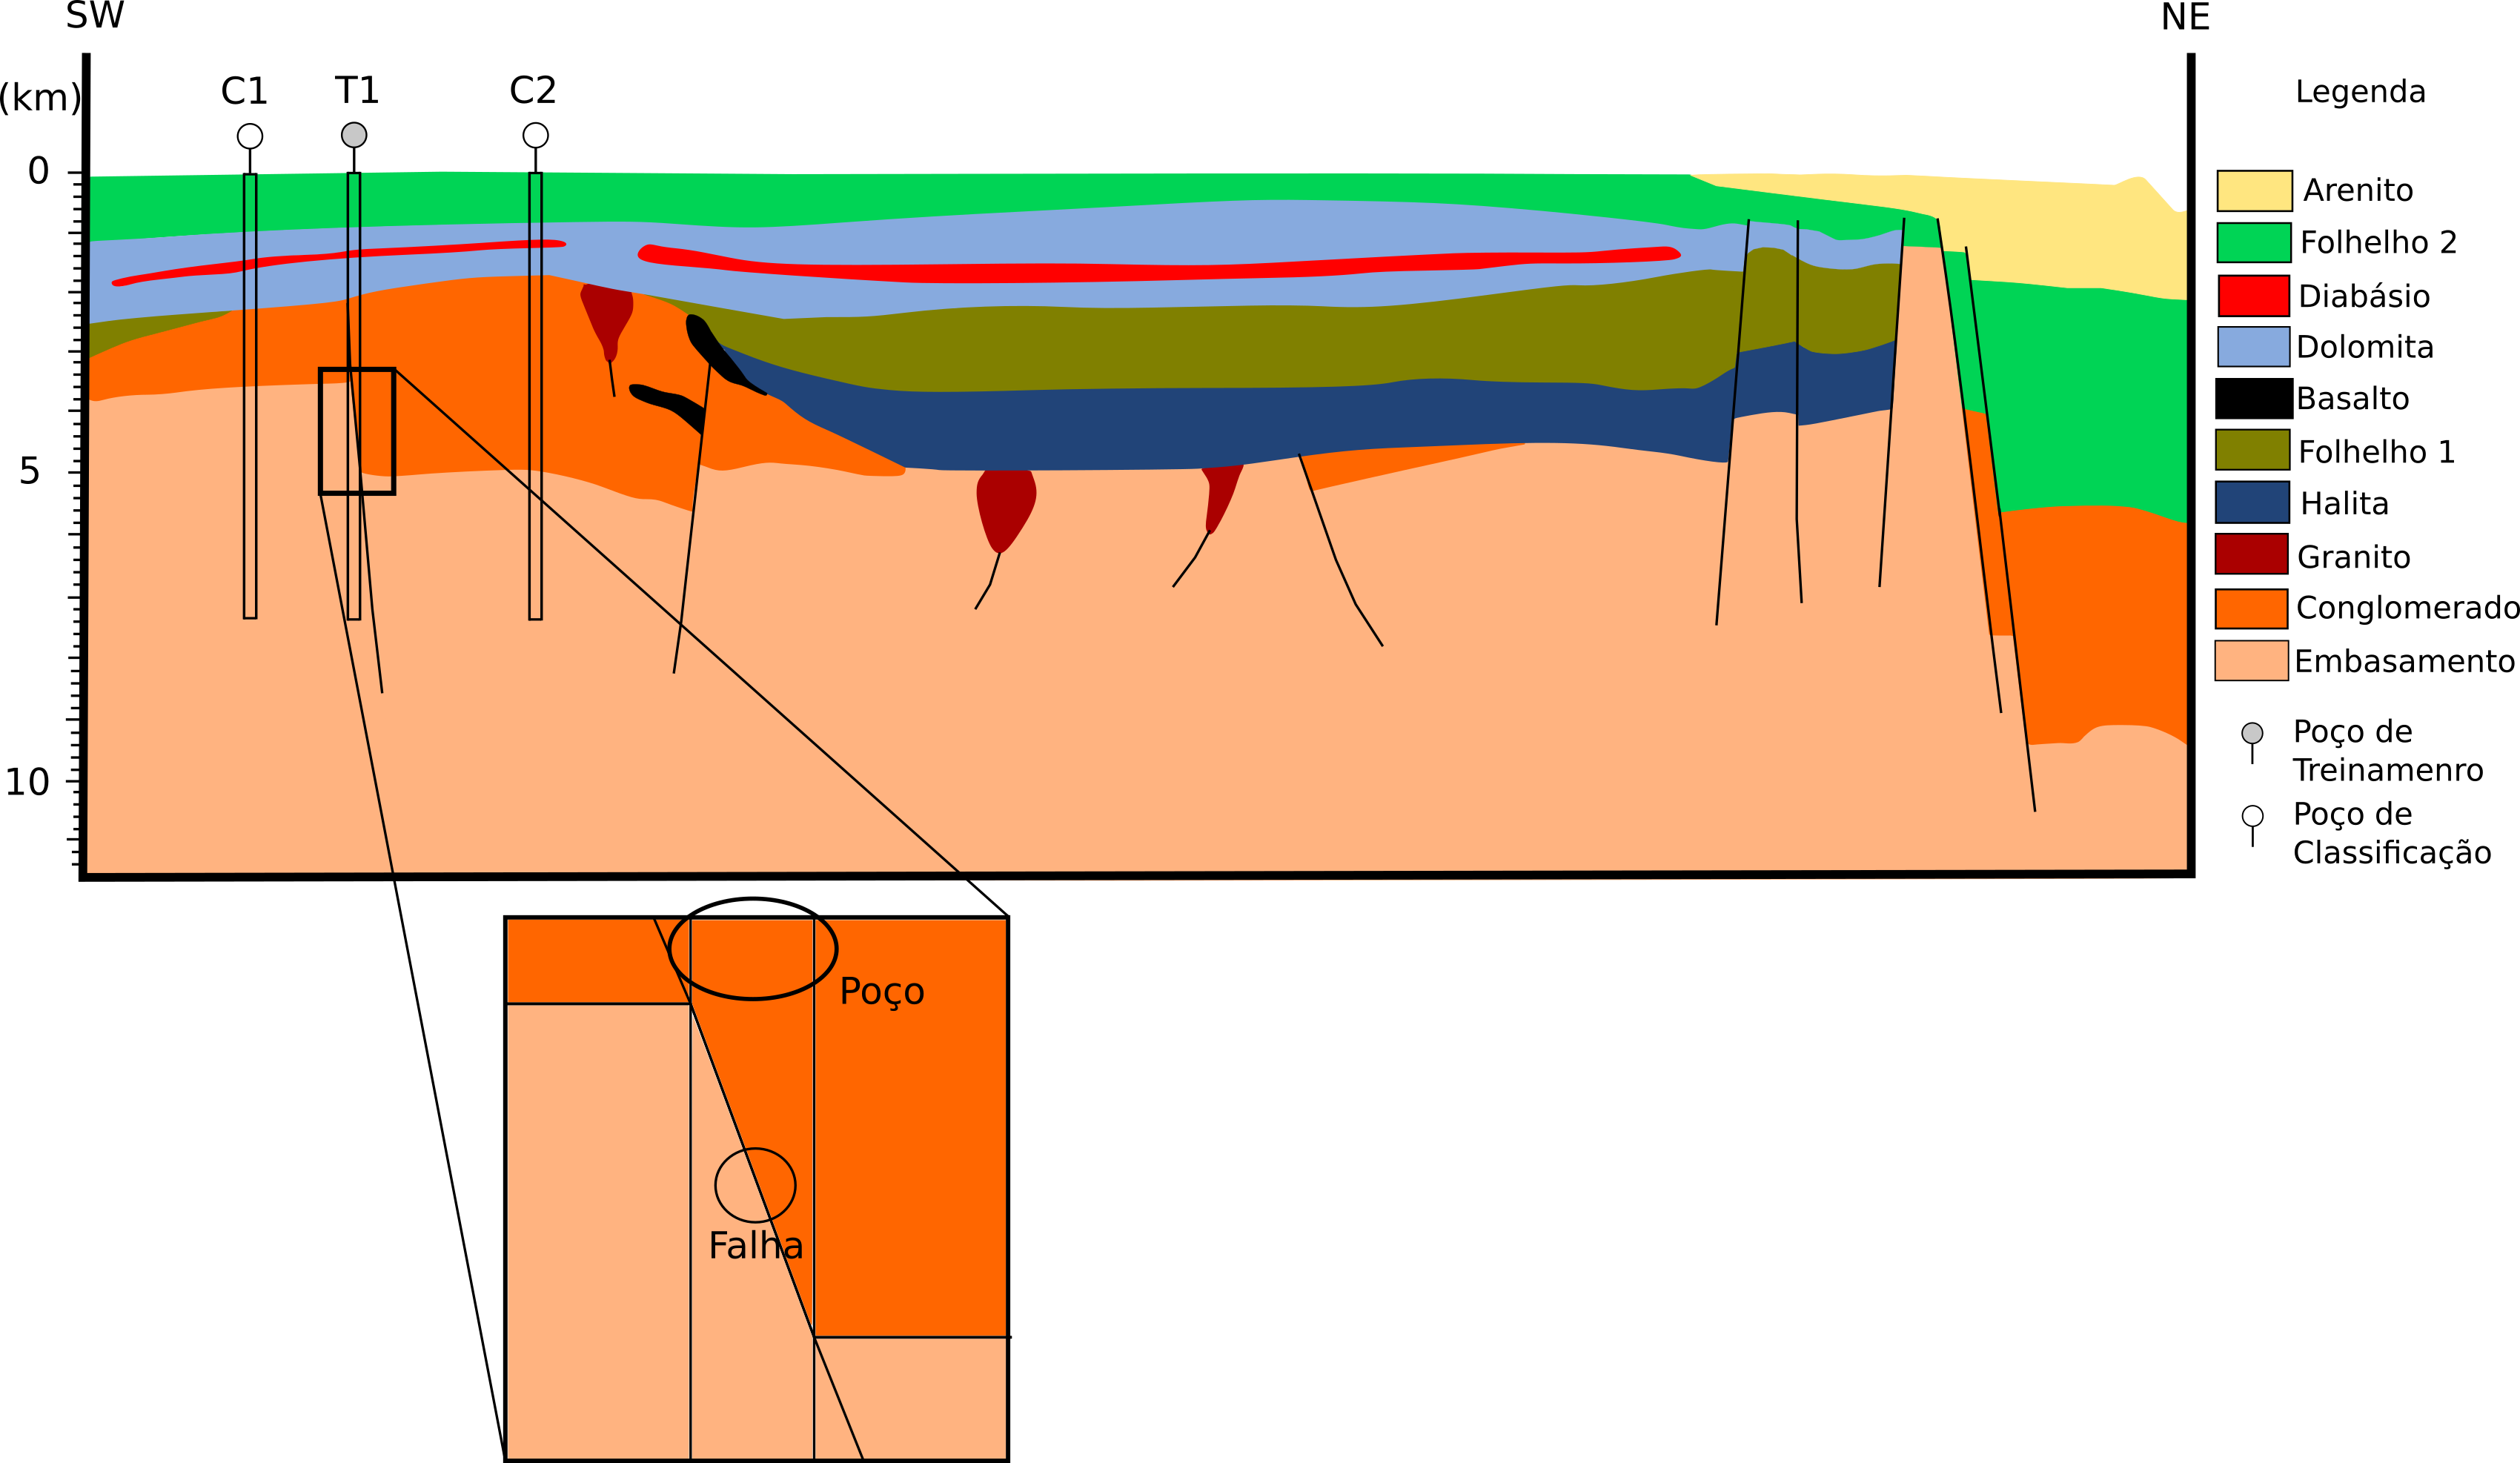
\includegraphics[scale=0.35]{Imagens/Modelo.png}
		\caption{Modelo Simplificado baseado em \cite{Sal2008}.}
		\label{modelo}
	\end{figure}
\end{frame}

\begin{frame}
	\frametitle{Modelo proposto}
	\begin{figure}[H]
		\centering
			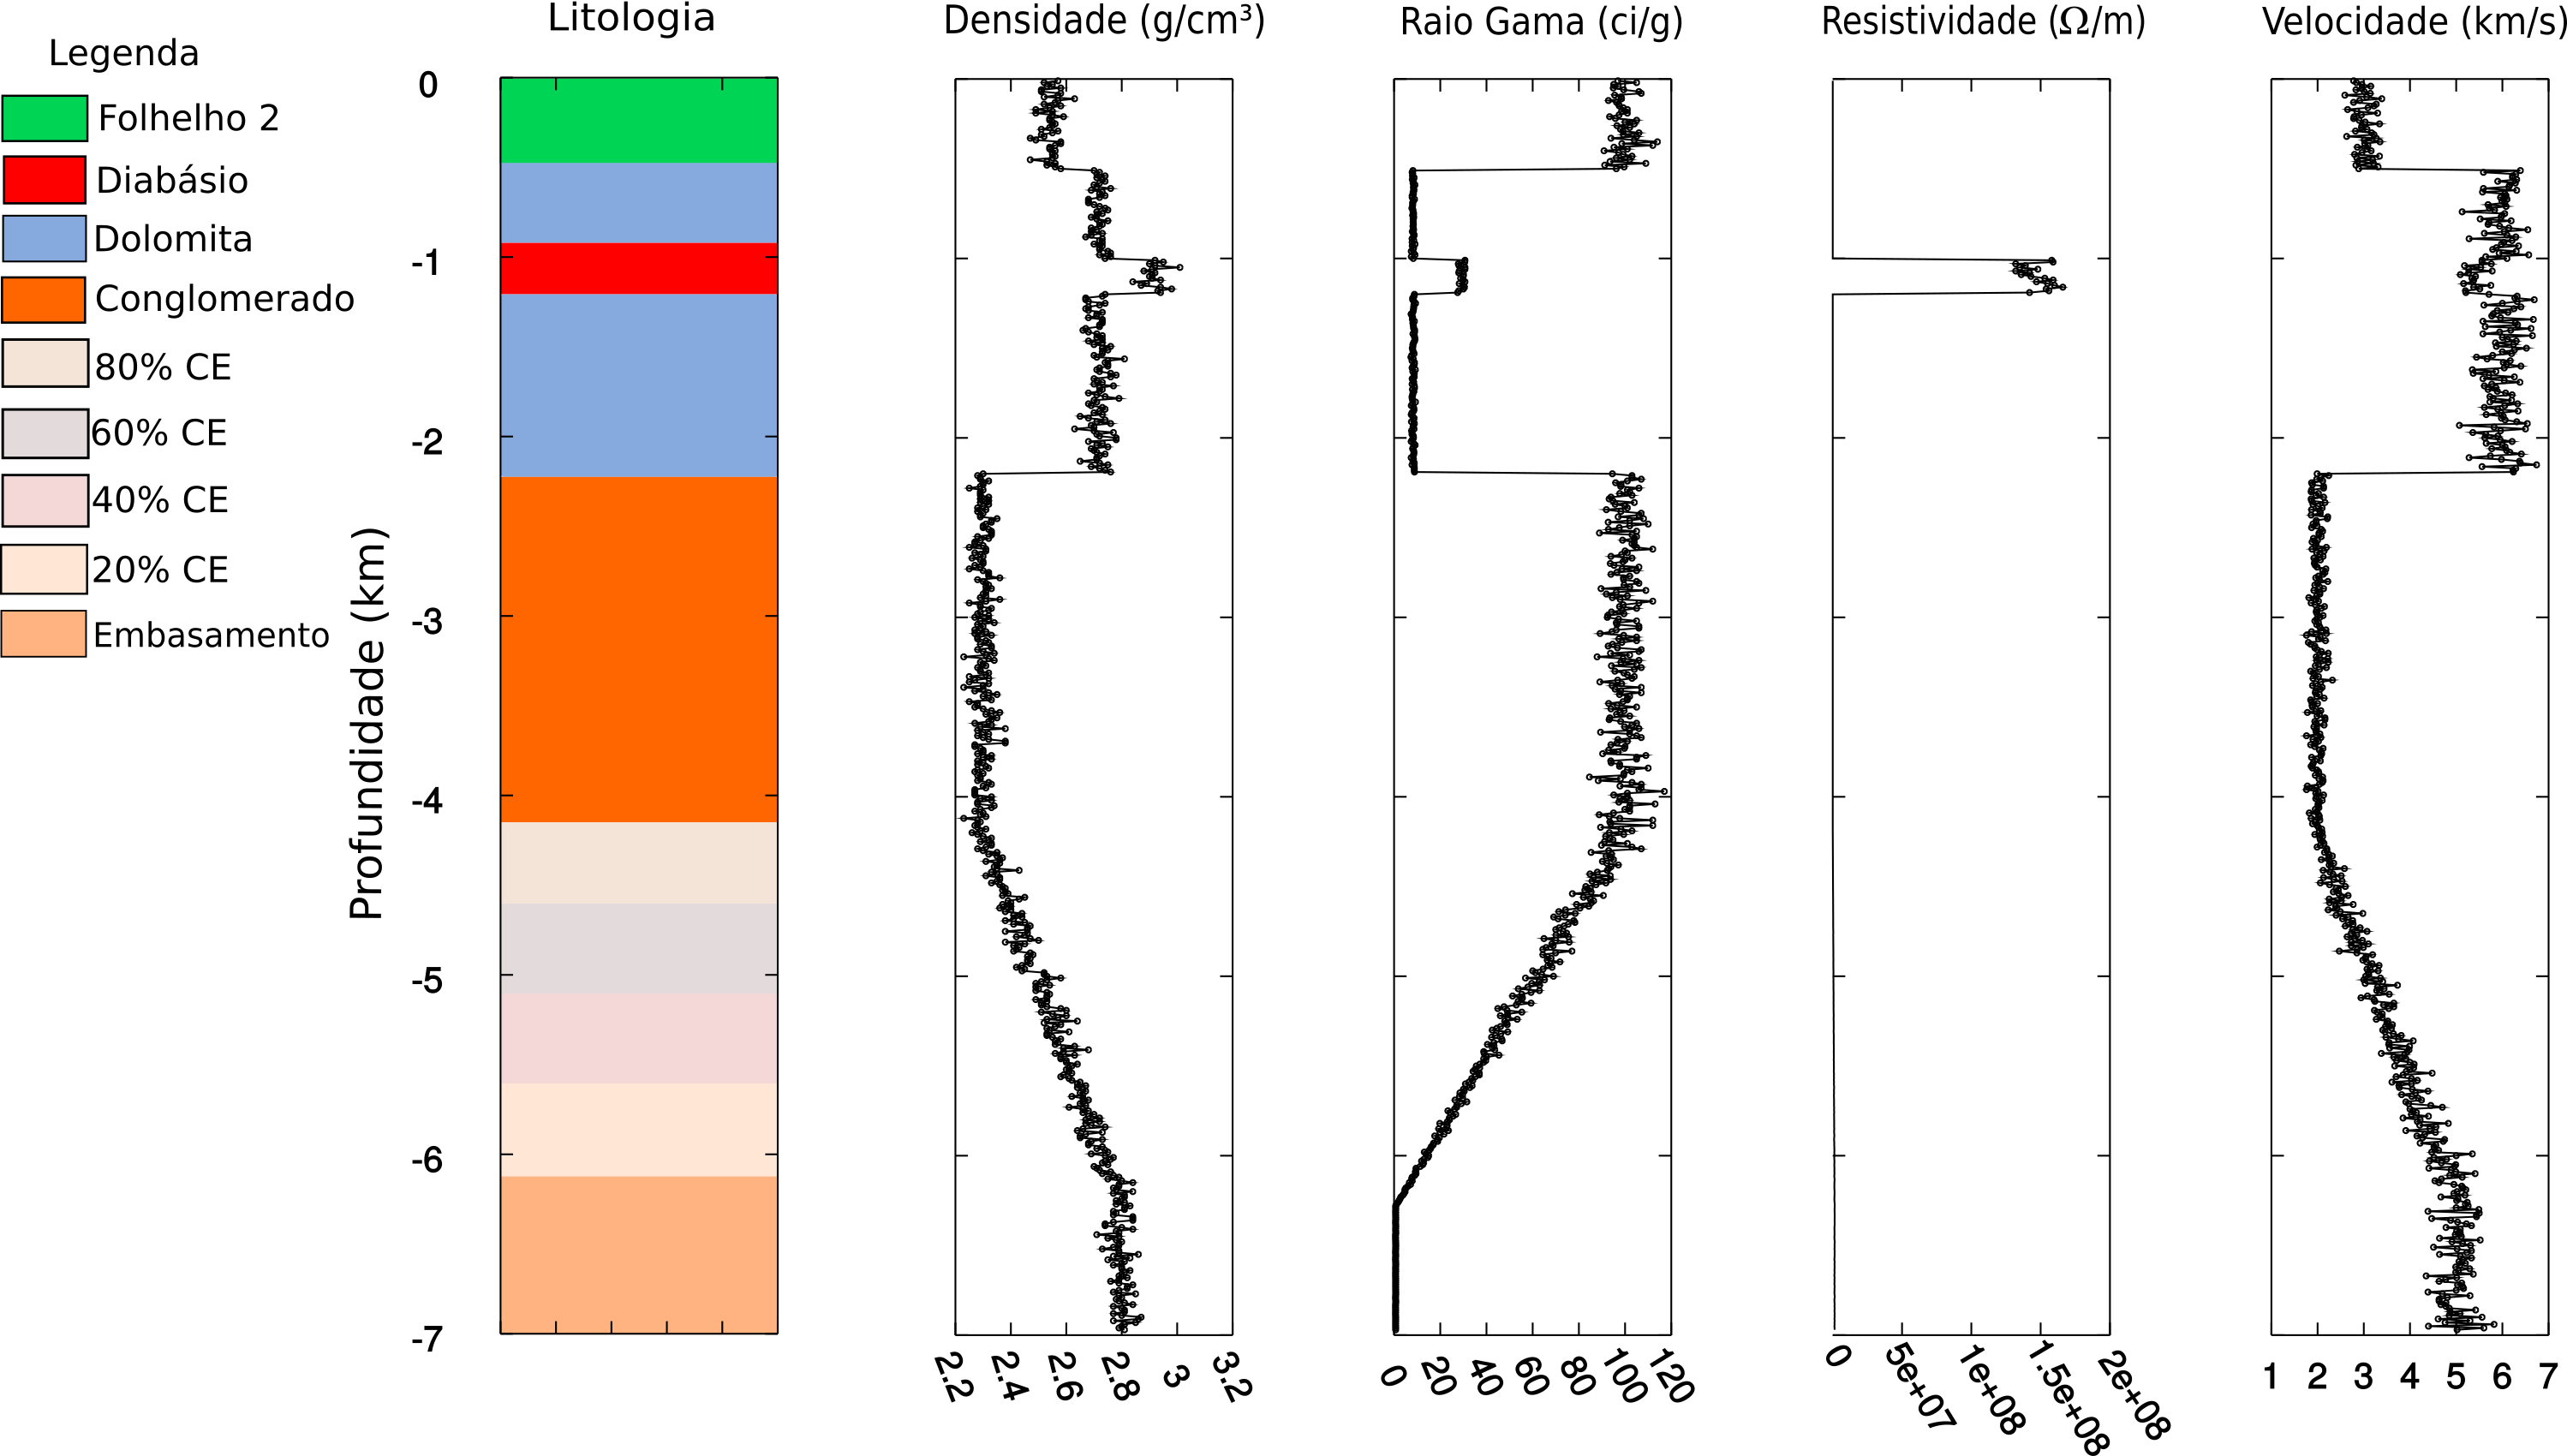
\includegraphics[scale=0.37]{Imagens/PocoT1.png}
		\caption{Dado de perfilagem sintético, T1. }
		\label{T1}
	\end{figure}
\end{frame}


\begin{frame}
	\frametitle{Modelo proposto}
	\begin{figure}[H]
		\centering
			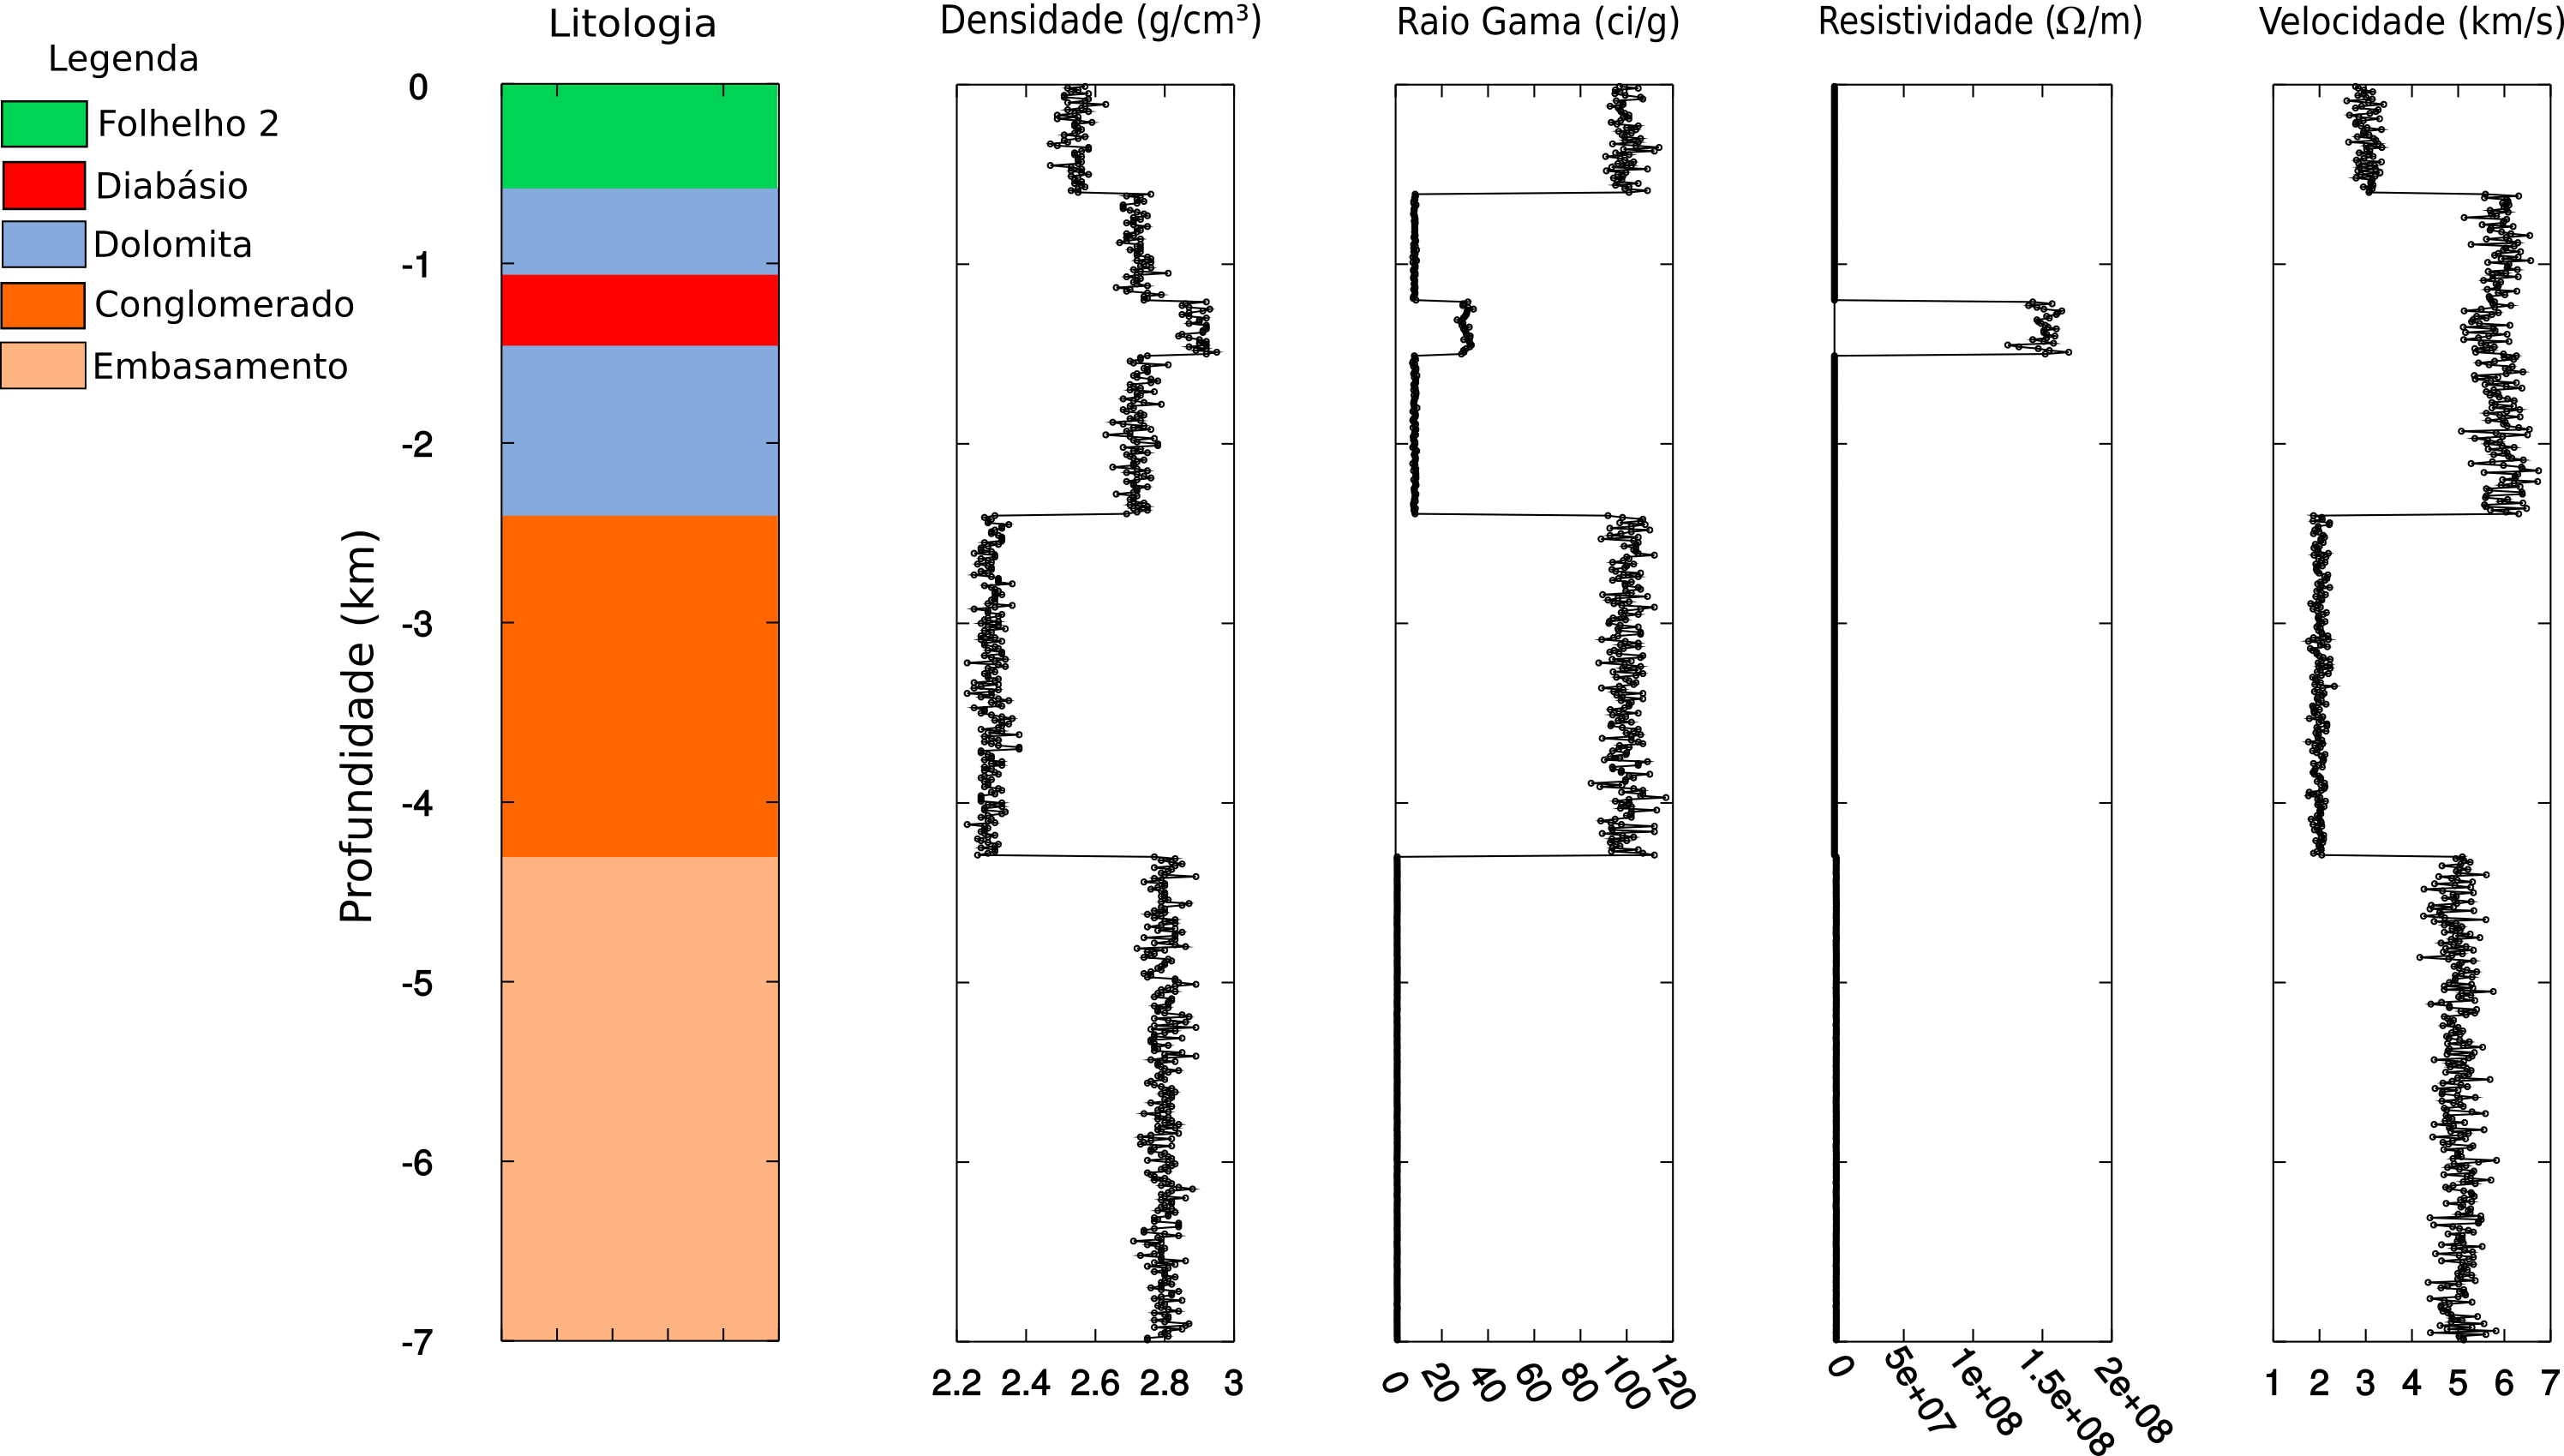
\includegraphics[scale=0.37]{Imagens/PocoC1.png}
		\caption{Dado de perfilagem sintético, C1.}
		\label{C1}
	\end{figure}
\end{frame}

\begin{frame}
	\frametitle{Modelo proposto}
	\begin{figure}[H]
		\centering
			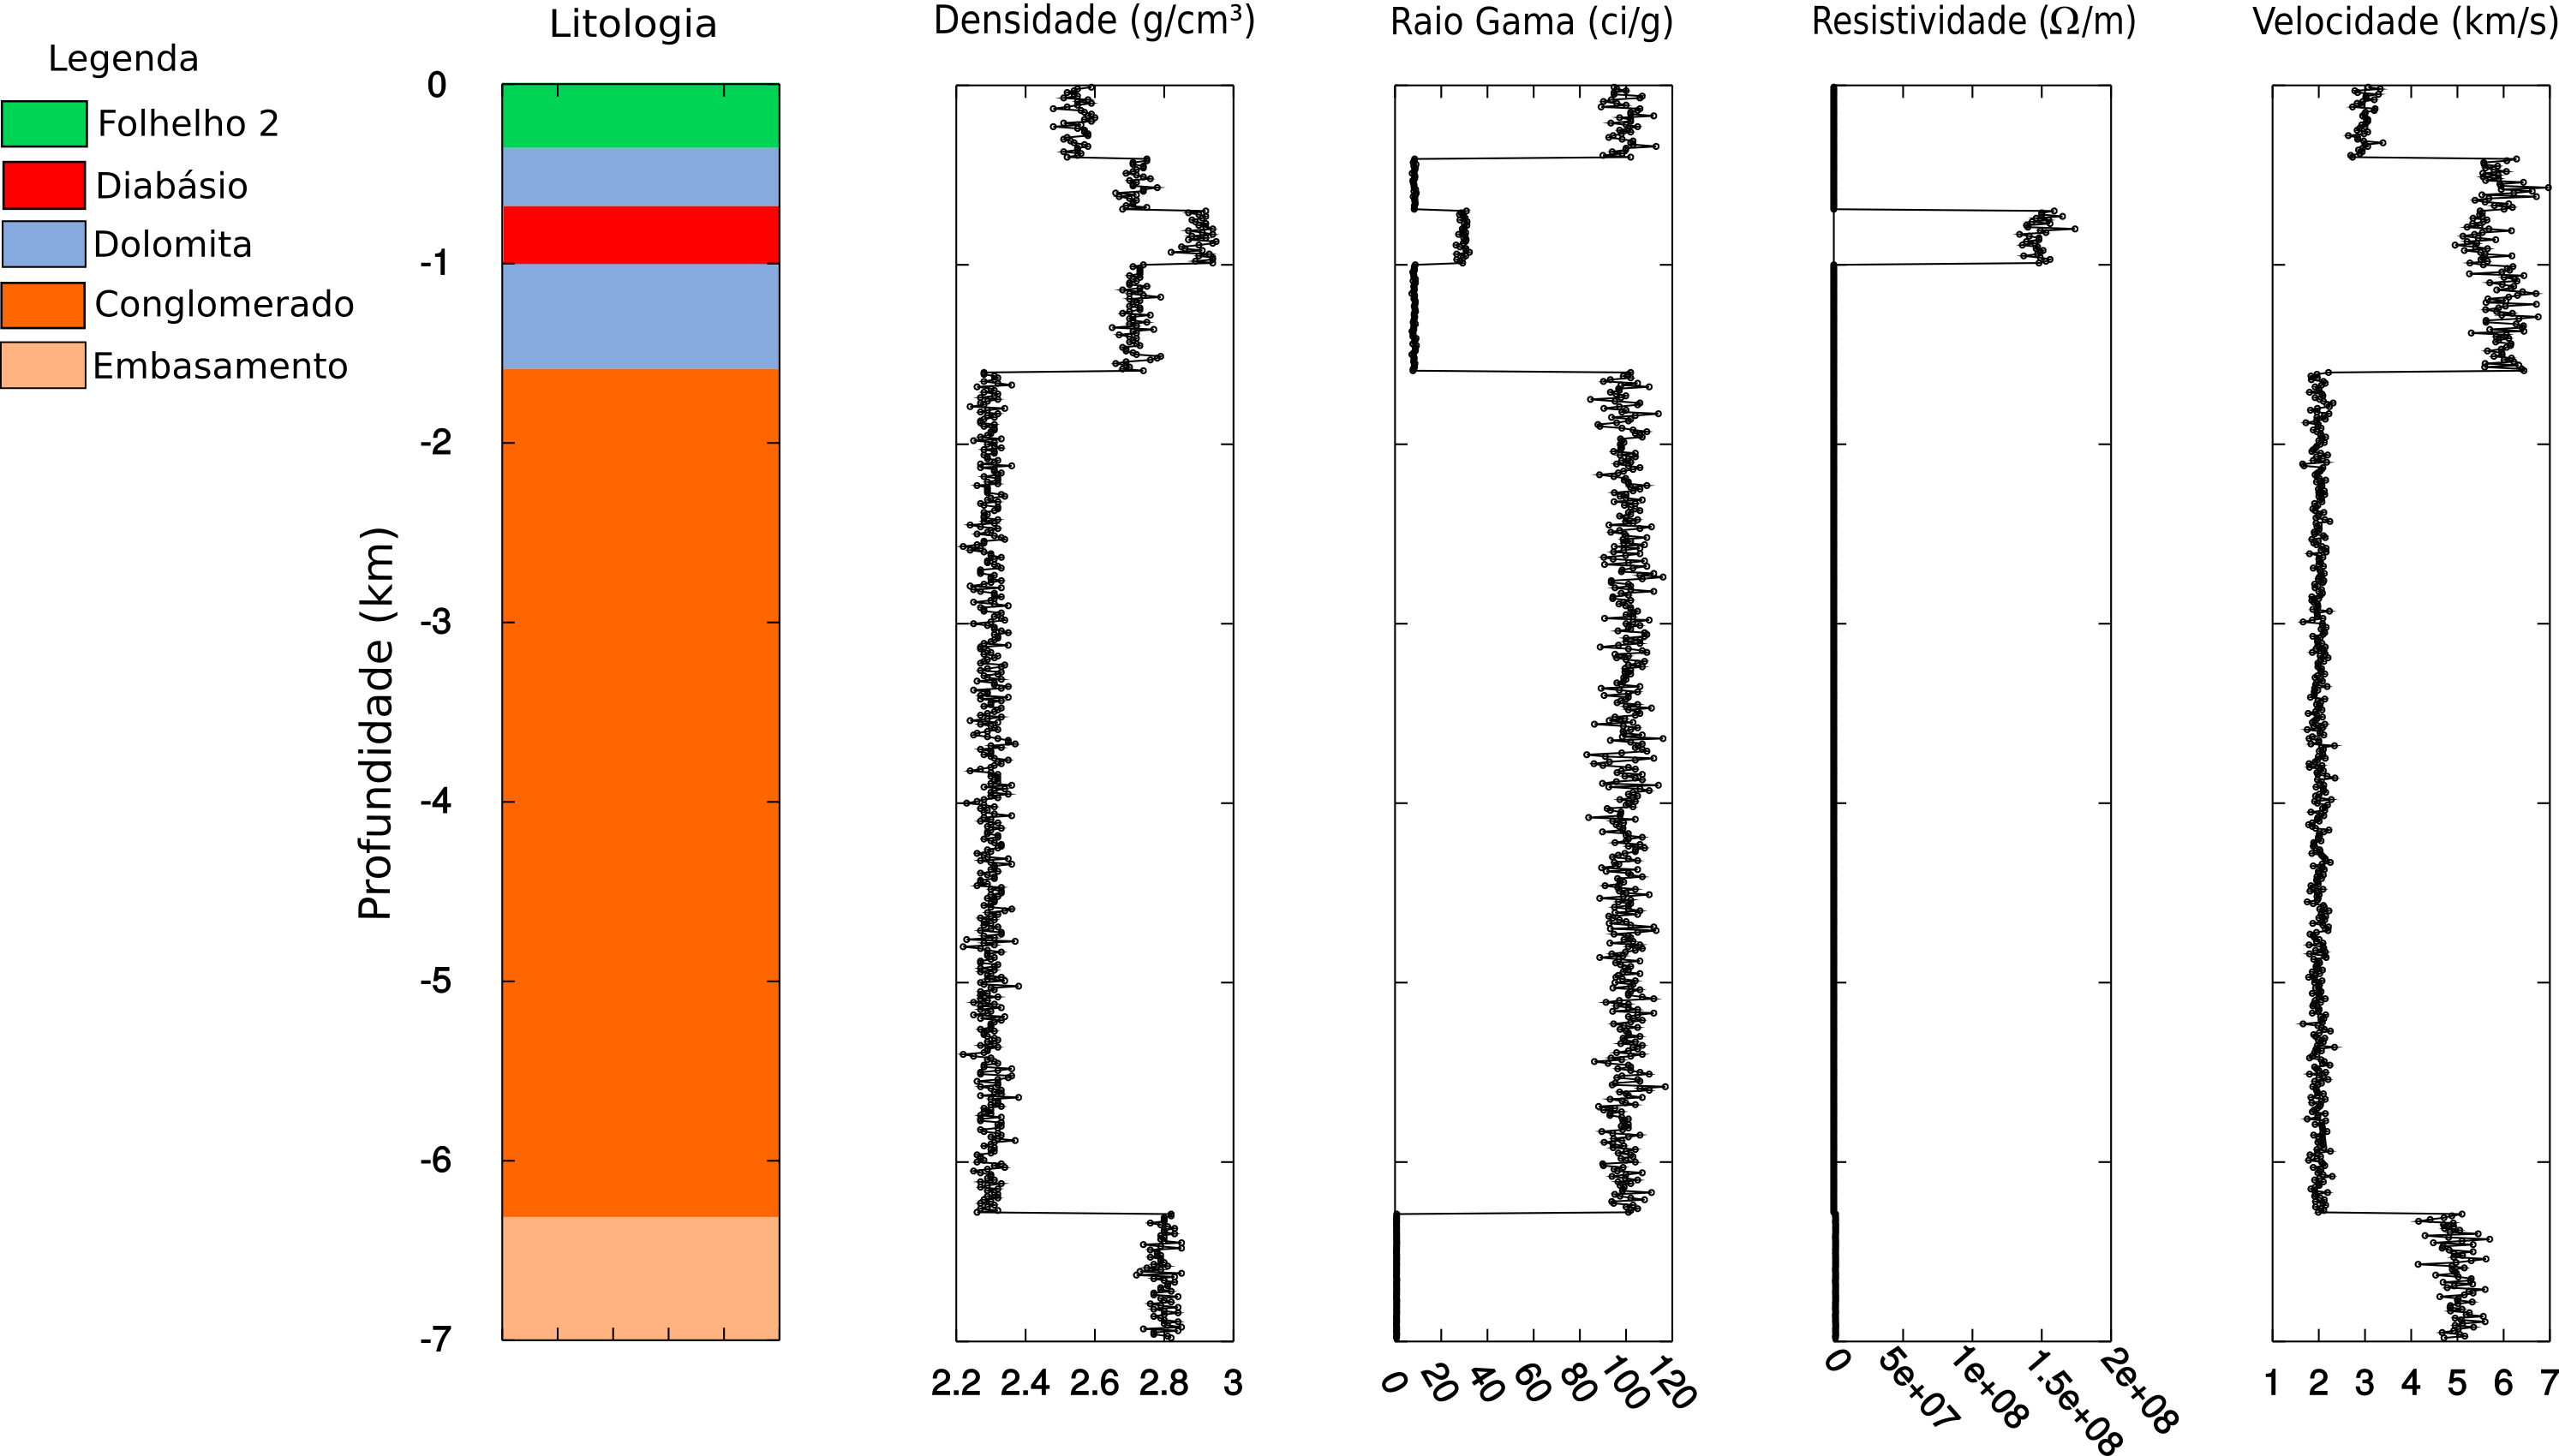
\includegraphics[scale=0.37]{Imagens/PocoC2.png}
		\caption{Dado de perfilagem sintético, C2.}
		\label{C2}
	\end{figure}
\end{frame}

\subsection{Clusterização}
\begin{frame}
	\frametitle{Clusterização do poço T1}
	\begin{figure}[H]
		\centering
			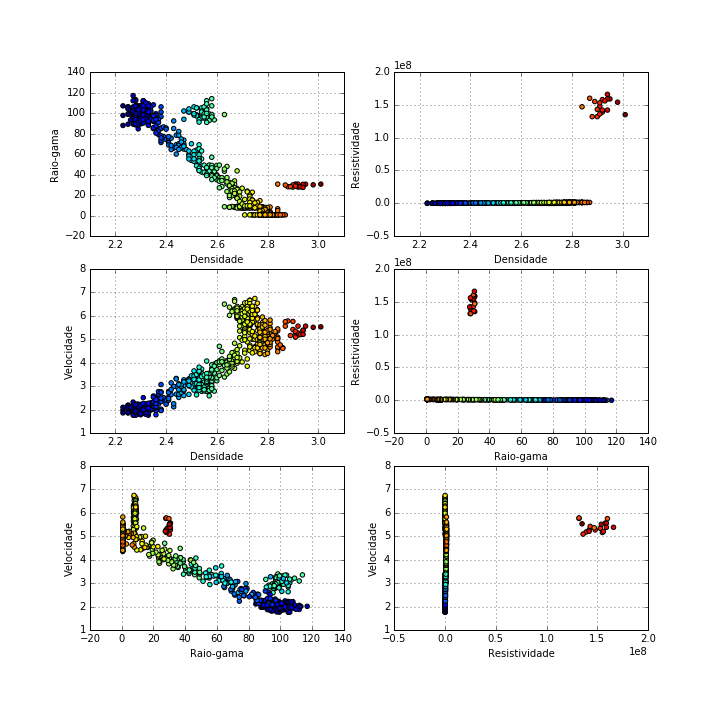
\includegraphics[scale=0.3]{Imagens/cluterpocoT1.png}
		\caption{Agrupamento de dados do poço T1.}
		\label{clusterT1}
	\end{figure} 
\end{frame}

\begin{frame}
	\frametitle{Clusterização do poço T1}
	\begin{figure}[H]
		\centering
		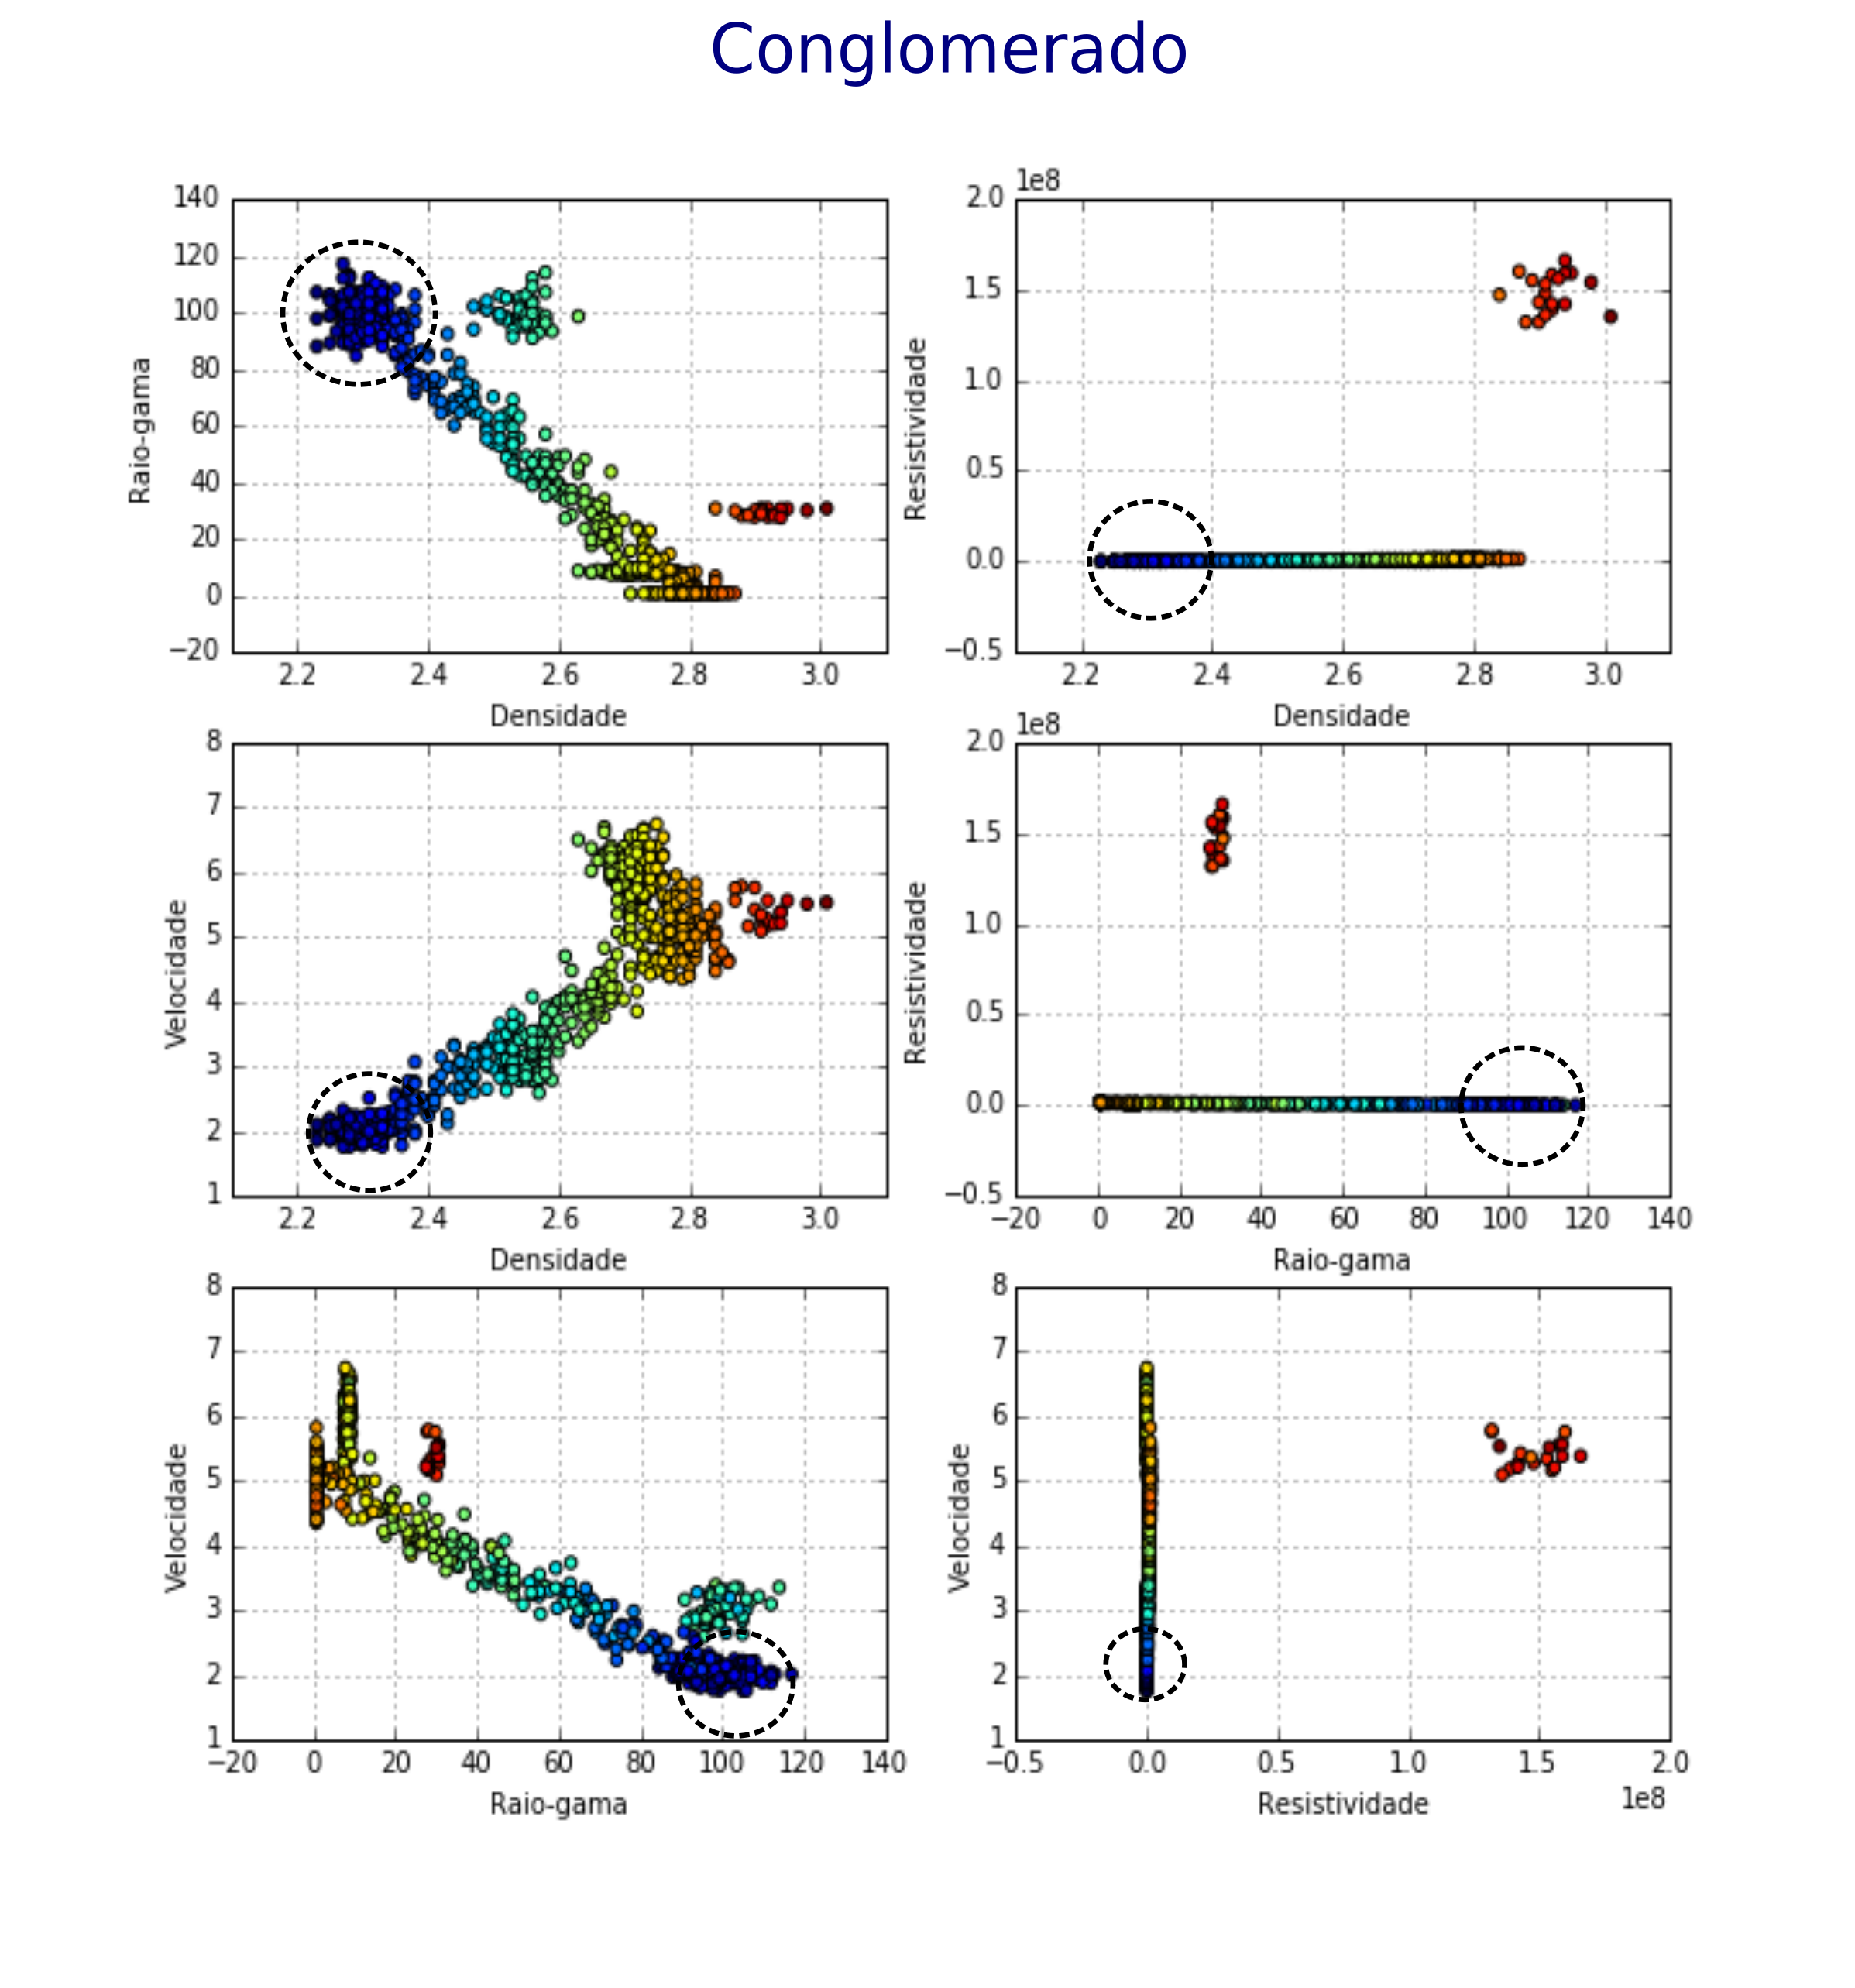
\includegraphics[scale=0.4]{Imagens/conglomerado.png}
		\caption{Agrupamento de dados do poço T1.}
	\end{figure} 
\end{frame}
\begin{frame}
	\frametitle{Clusterização do poço T1}
	\begin{figure}[H]
		\centering
		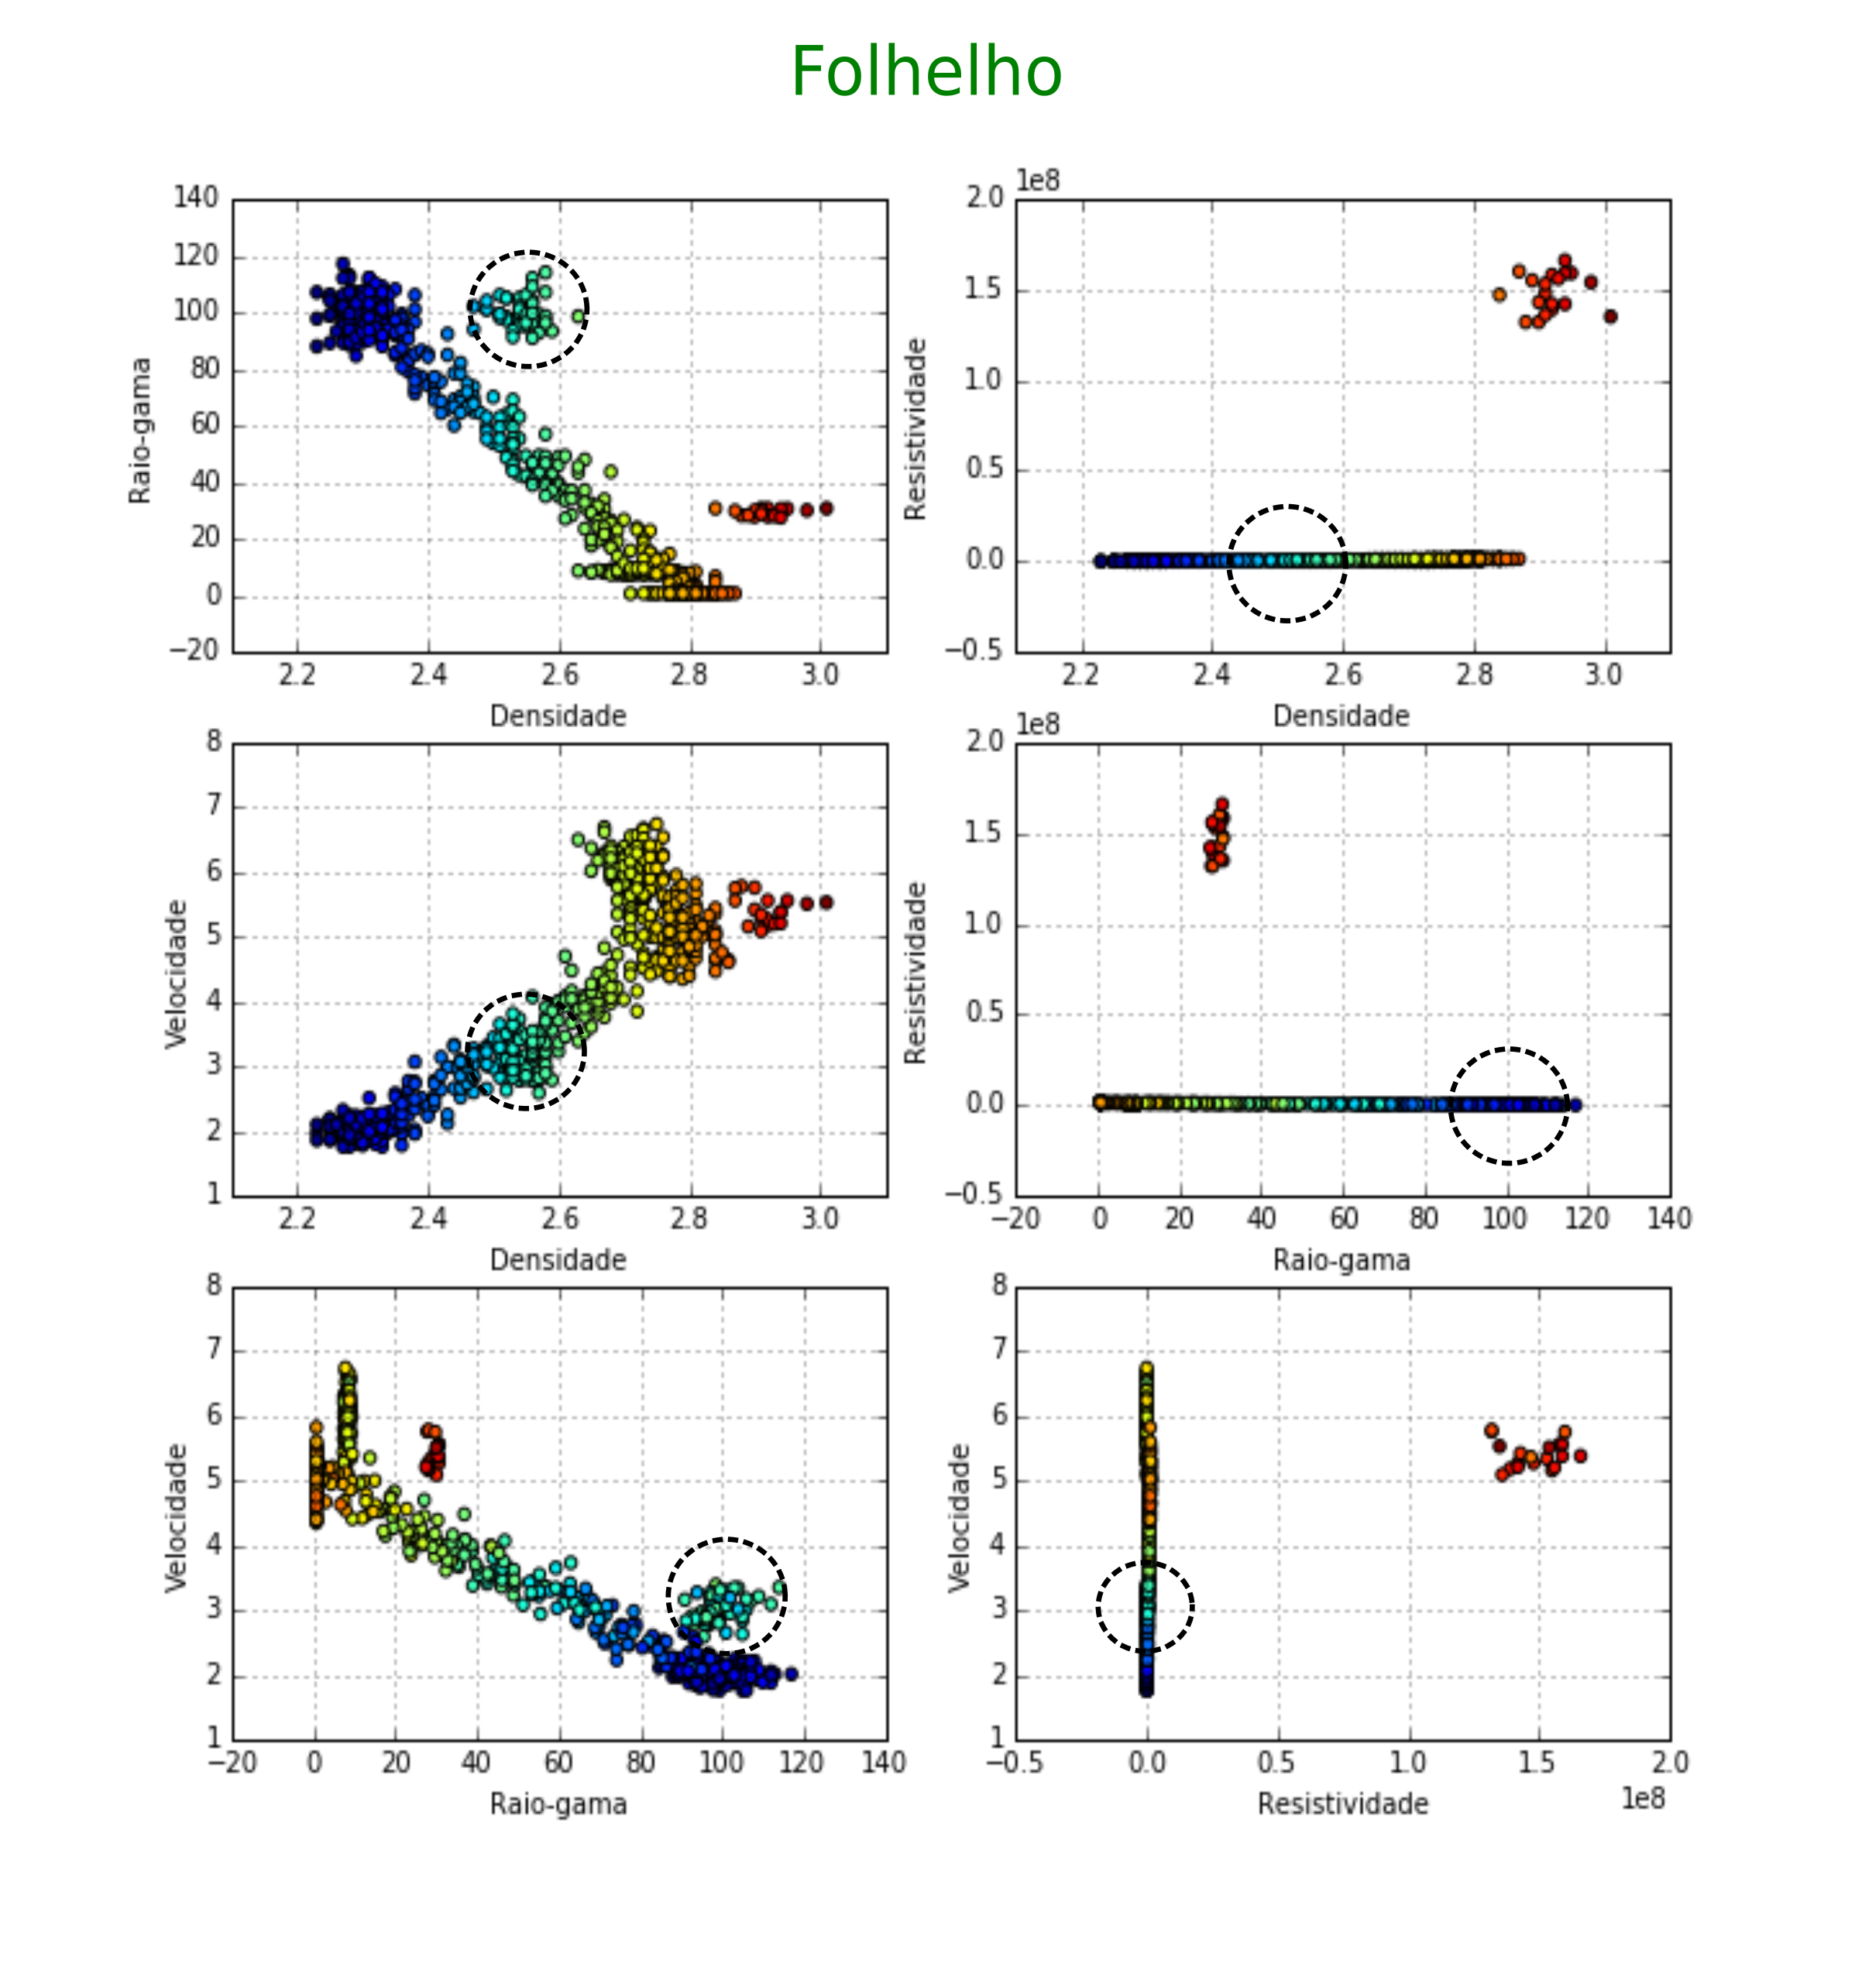
\includegraphics[scale=0.4]{Imagens/folhelho.png}
		\caption{Agrupamento de dados do poço T1.}
	\end{figure} 
\end{frame}
\begin{frame}
	\frametitle{Clusterização do poço T1}
	\begin{figure}[H]
		\centering
		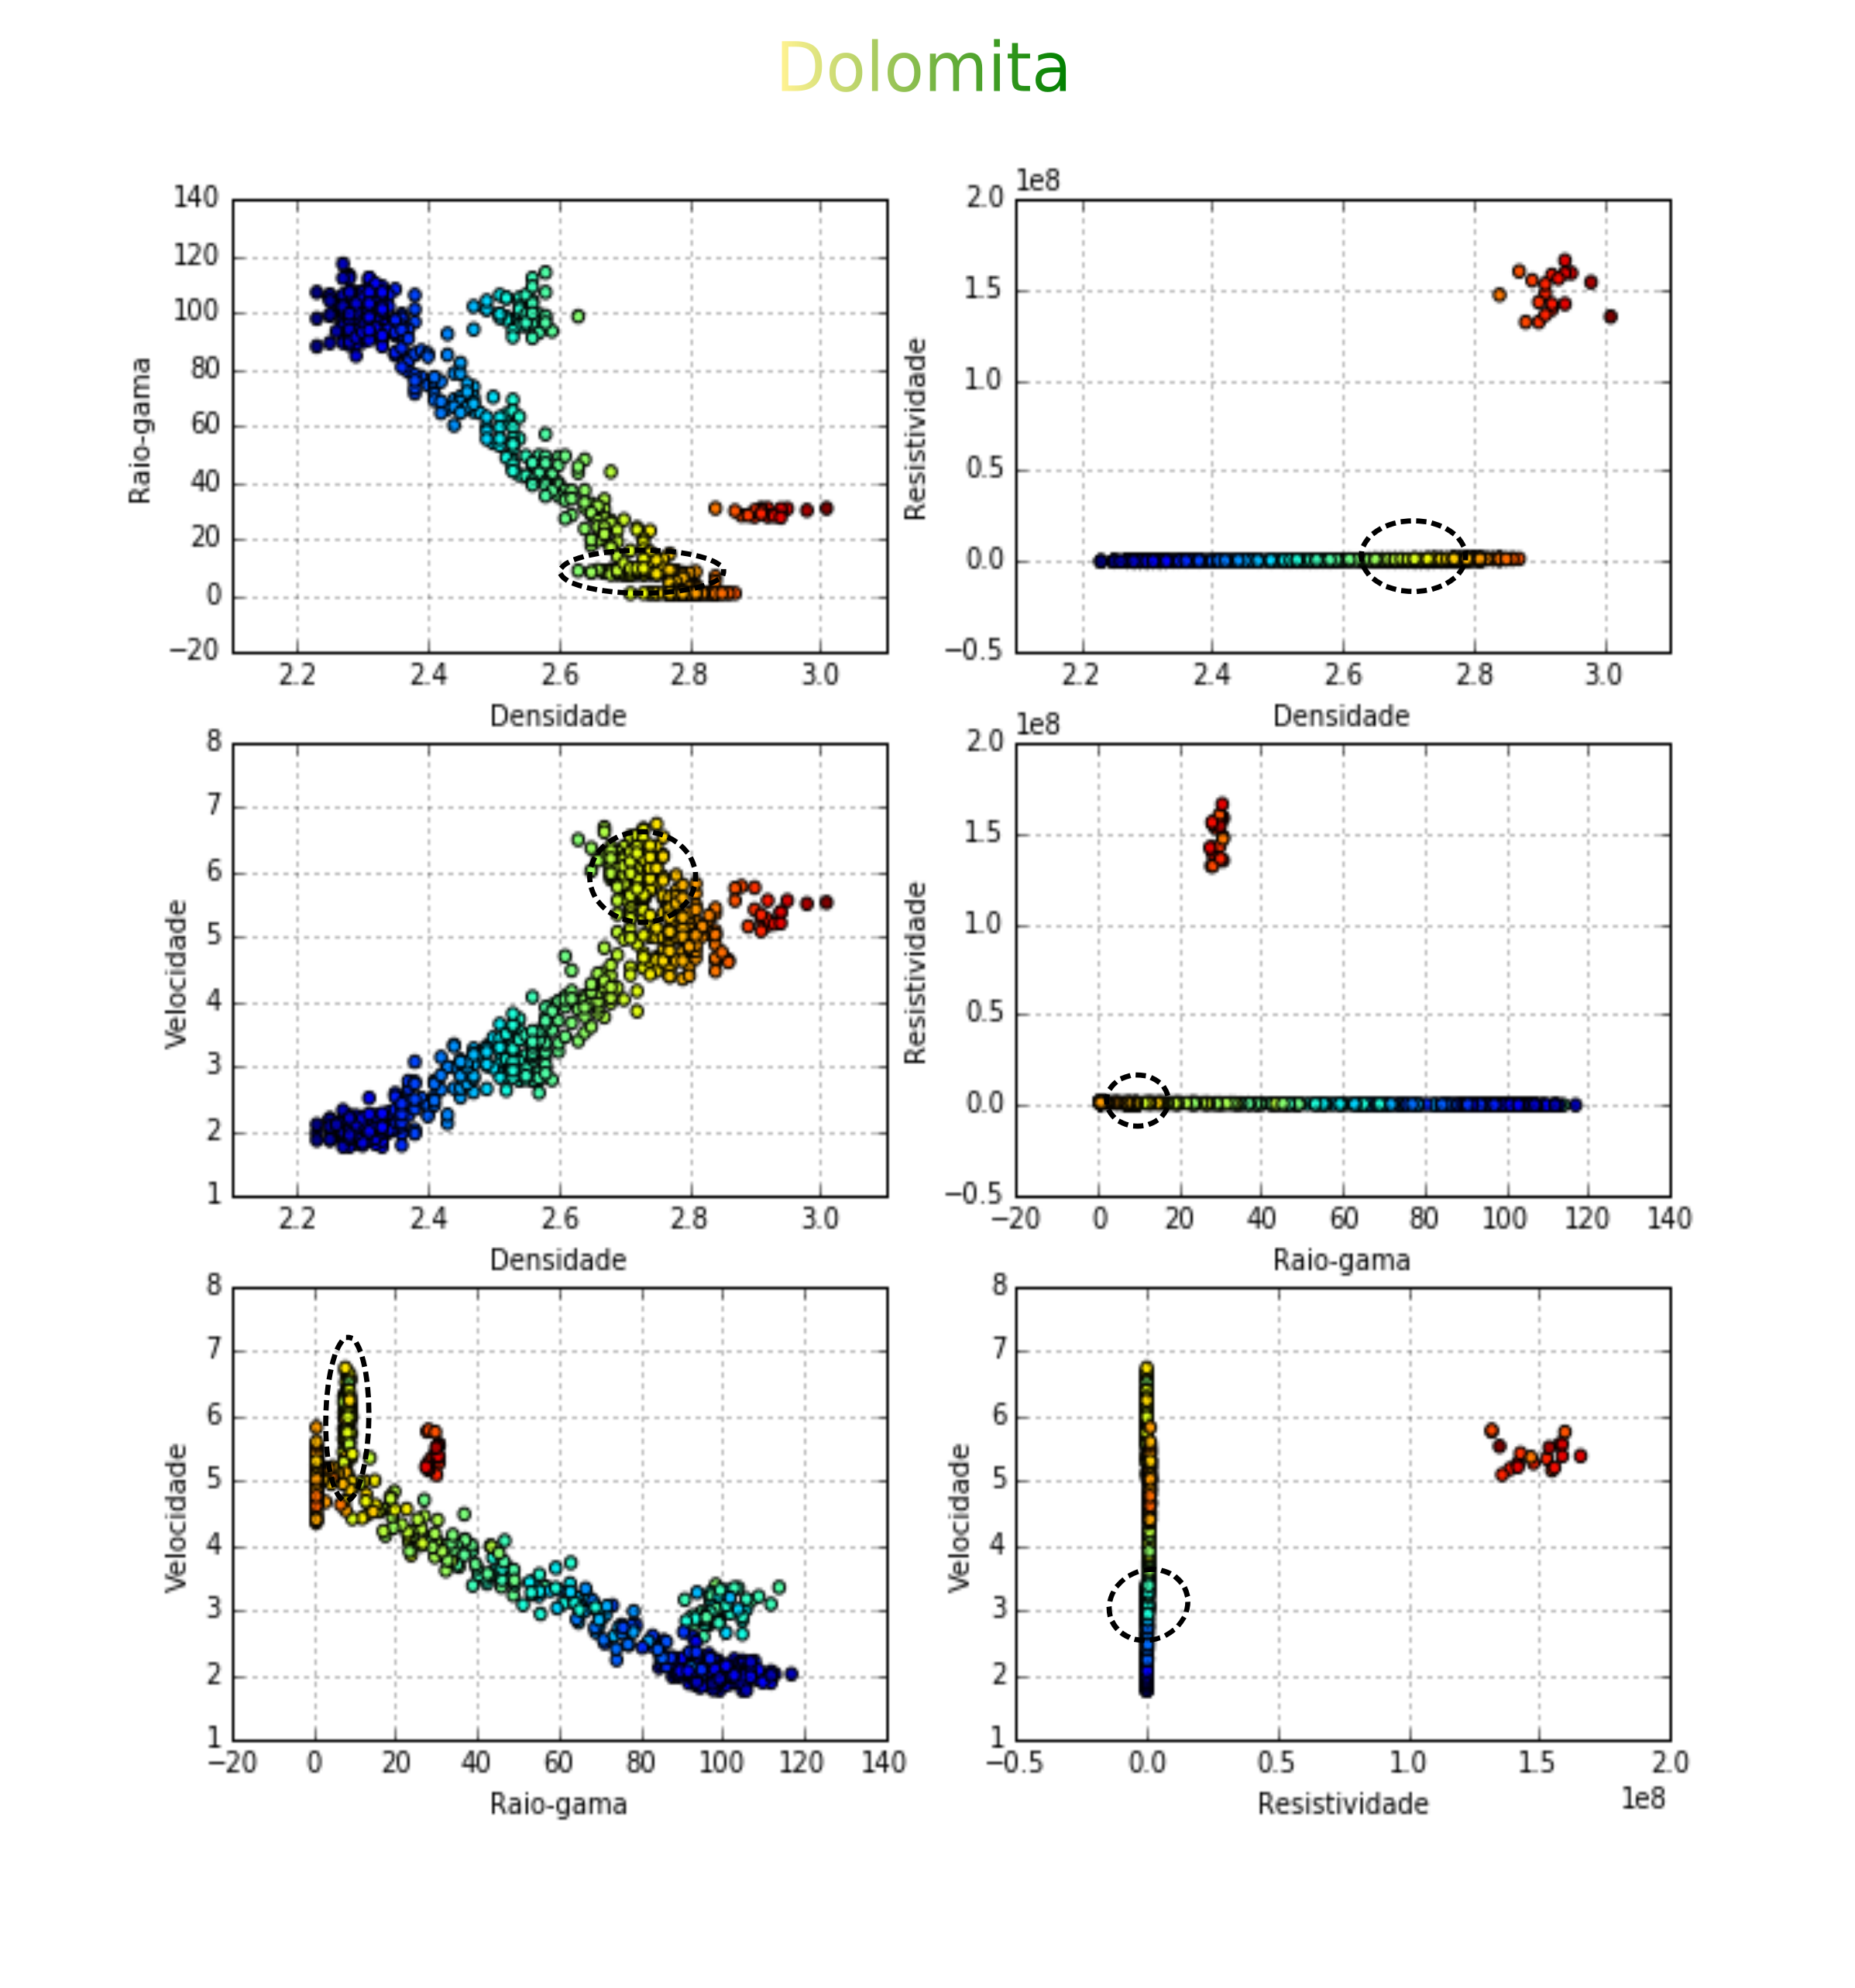
\includegraphics[scale=0.3]{Imagens/dolomita.png}
		\caption{Agrupamento de dados do poço T1.}

	\end{figure} 
\end{frame}
\begin{frame}
	\frametitle{Clusterização do poço T1}
	\begin{figure}[H]
		\centering
		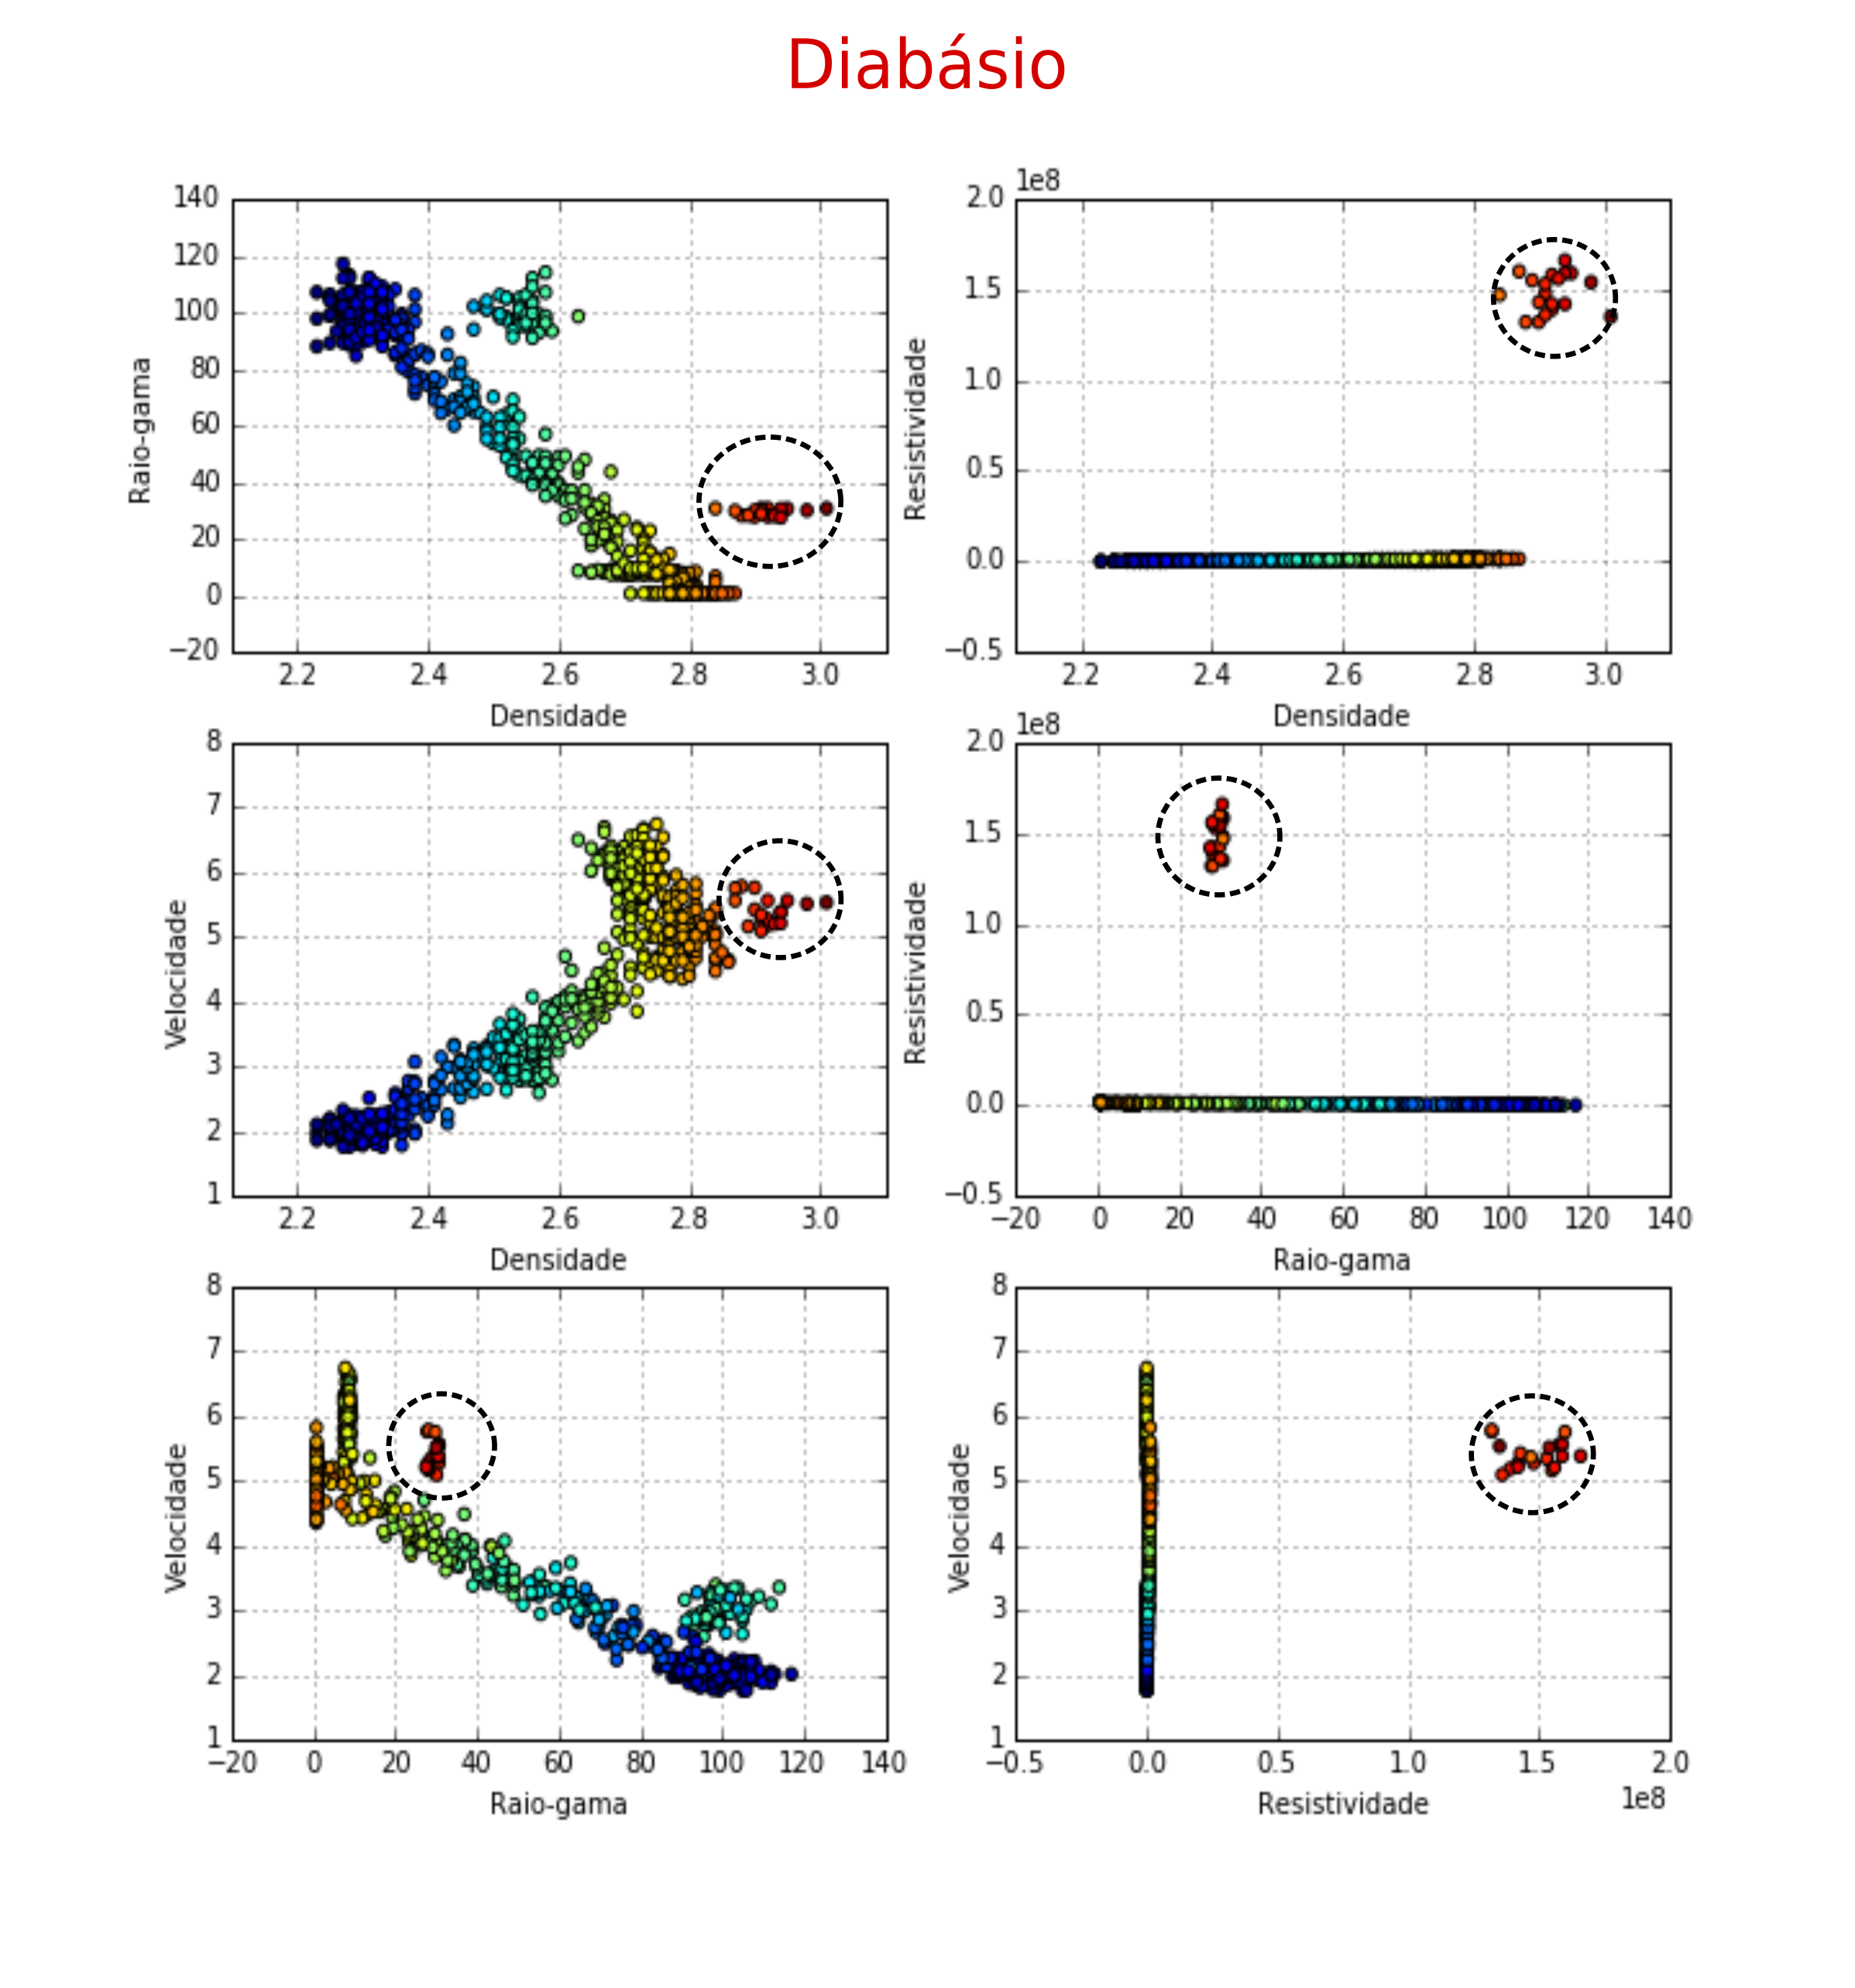
\includegraphics[scale=0.4]{Imagens/diabasio.png}
		\caption{Agrupamento de dados do poço T1.}
	\end{figure} 
\end{frame}
\begin{frame}
	\frametitle{Clusterização do poço T1}
	\begin{figure}[H]
		\centering
		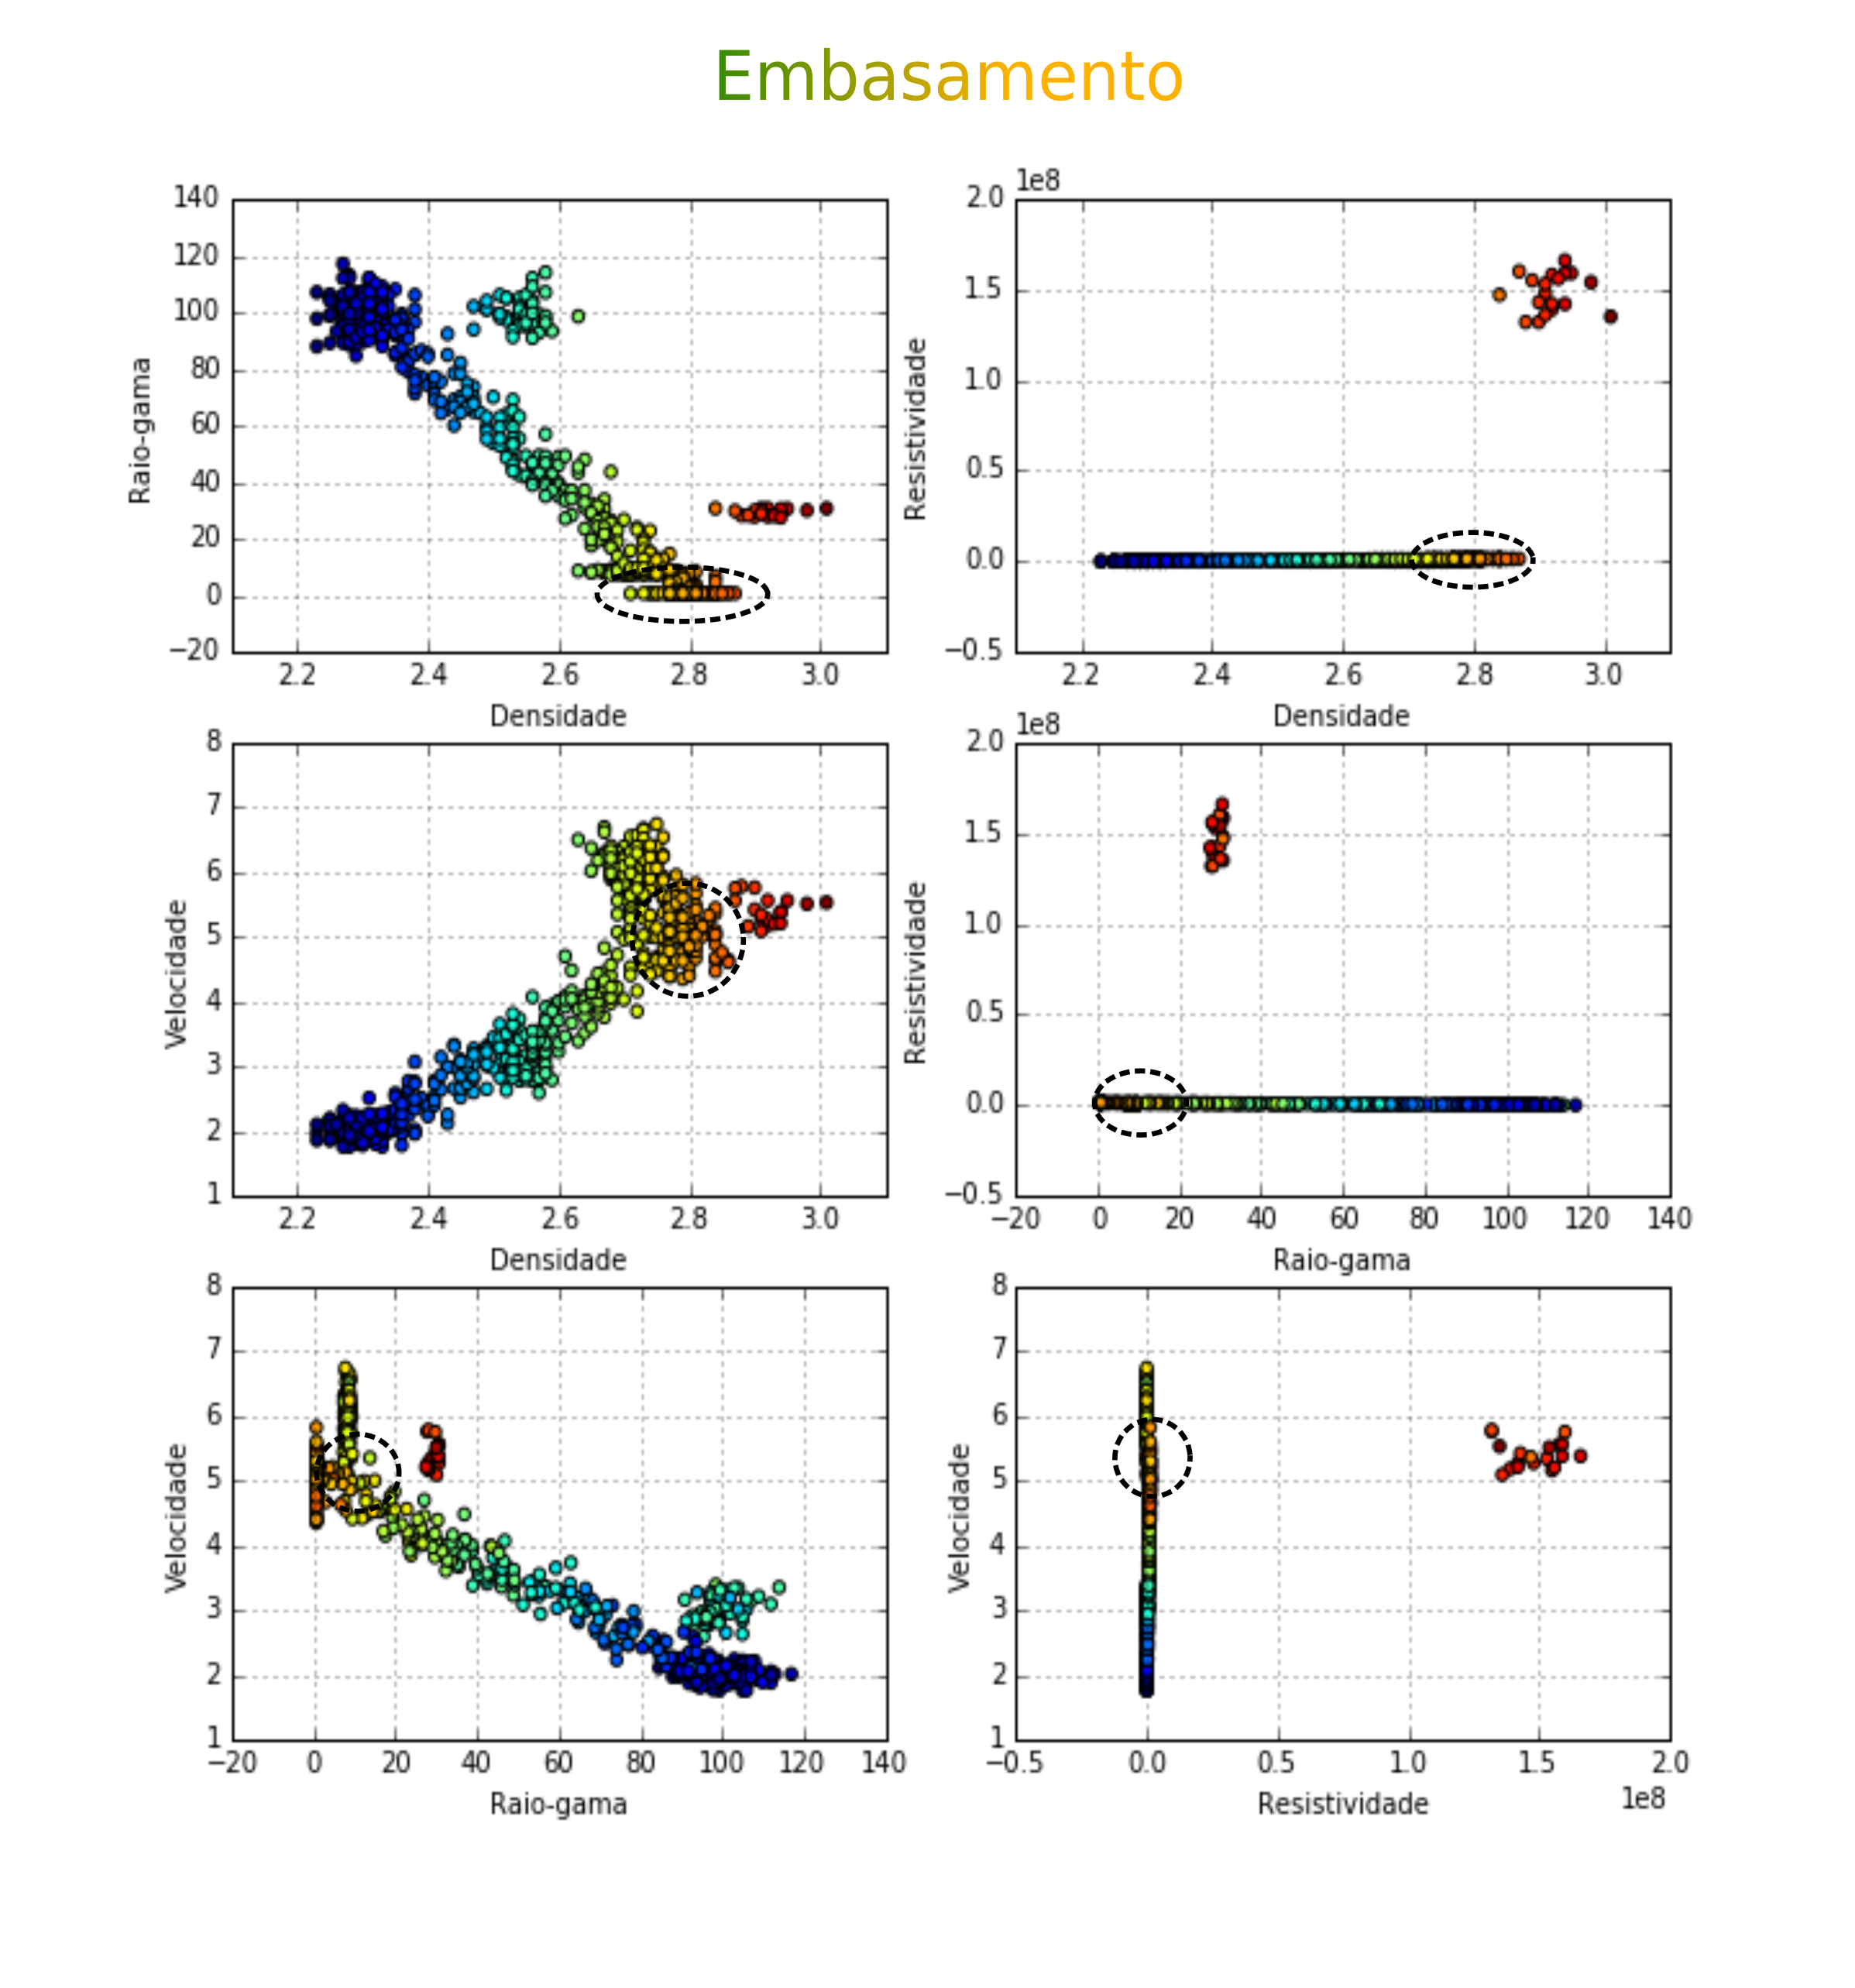
\includegraphics[scale=0.4]{Imagens/embasamento.png}
		\caption{Agrupamento de dados do poço T1.}
		\label{clusterT1}
	\end{figure} 
\end{frame}

\begin{frame}
	\frametitle{Clusterização do poço C1}
	\begin{figure}[H]
		\centering
			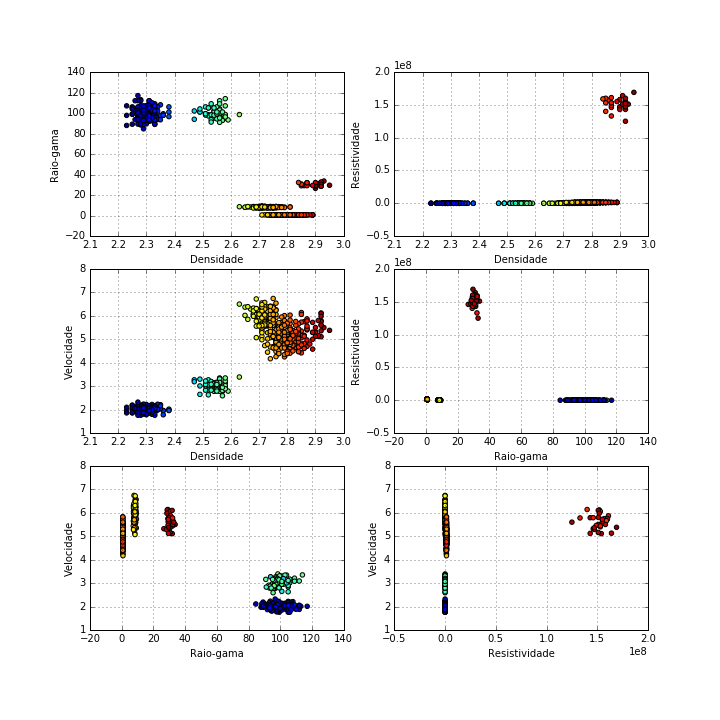
\includegraphics[scale=0.3]{Imagens/cluterpocoC1.png}
		\caption{Agrupamento de dados do poço C1.}
		\label{clusterC1}
	\end{figure} 
\end{frame}

\begin{frame}
	\frametitle{Clusterização do poço C1}
	\begin{figure}[H]
		\centering
		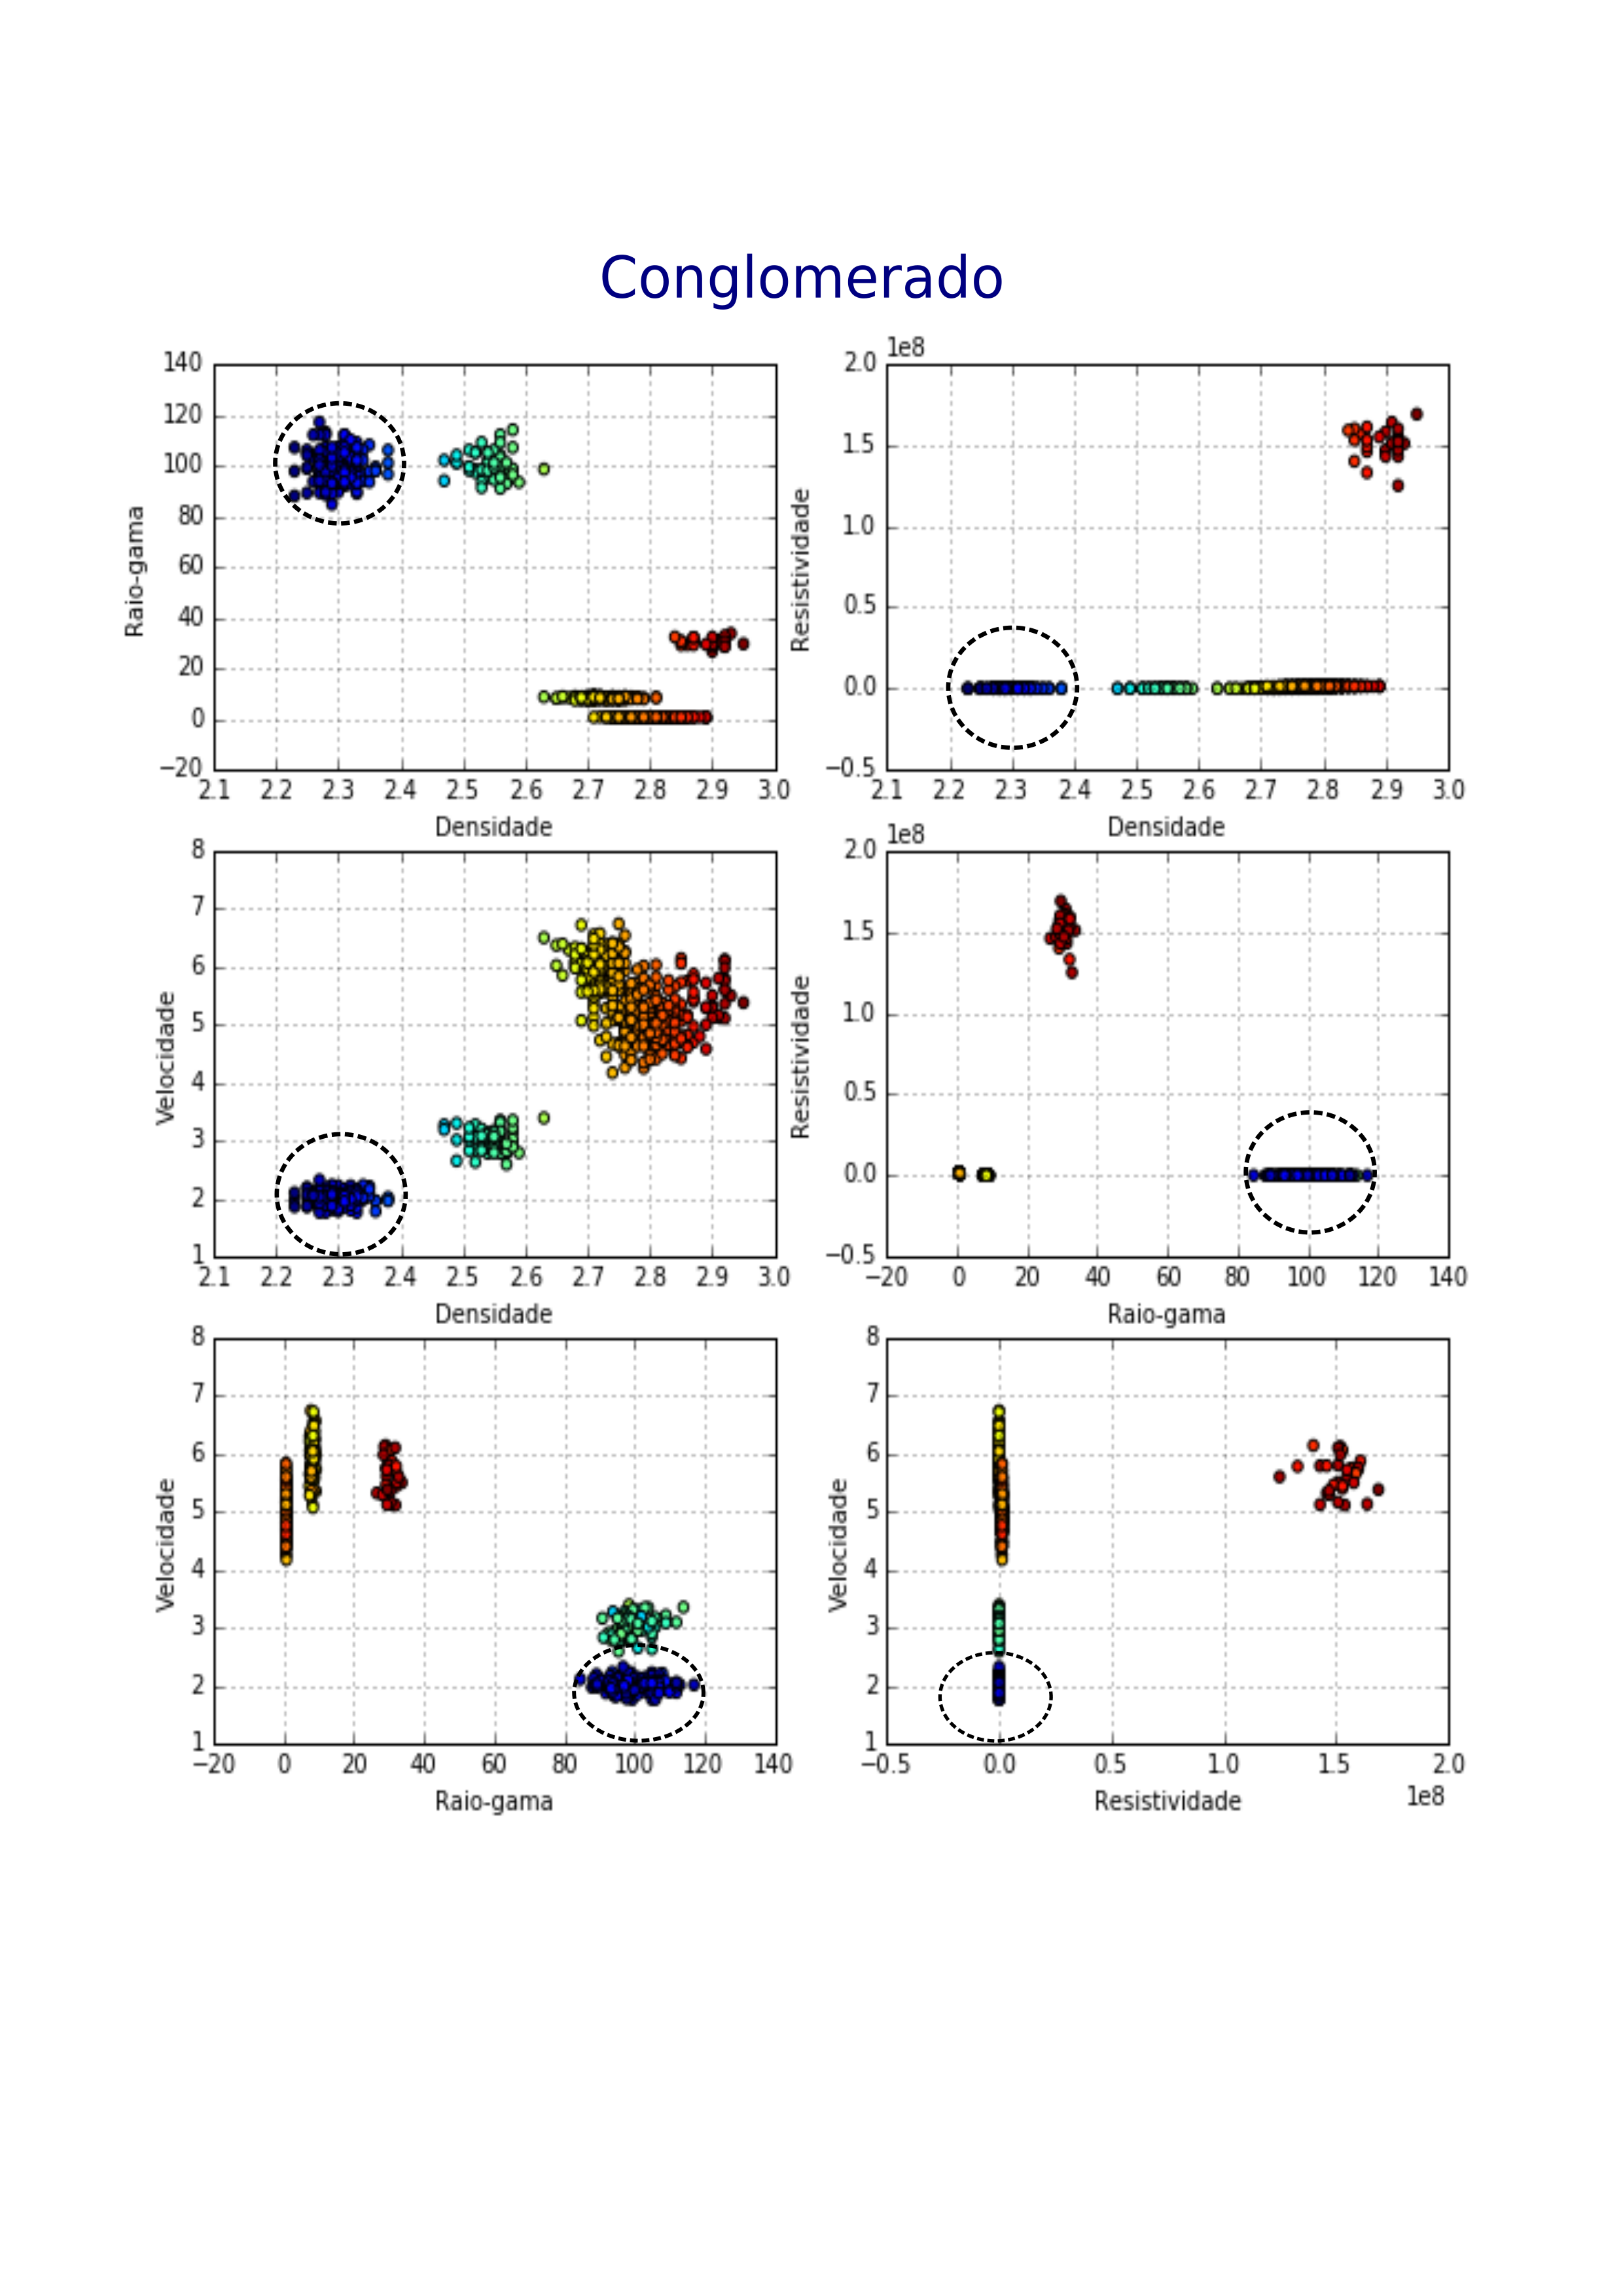
\includegraphics[scale=0.3]{Imagens/conglomeradoC1.png}
		\caption{Agrupamento de dados do poço C1.}
	\end{figure} 
\end{frame}

\begin{frame}
	\frametitle{Clusterização do poço C1}
	\begin{figure}[H]
		\centering
		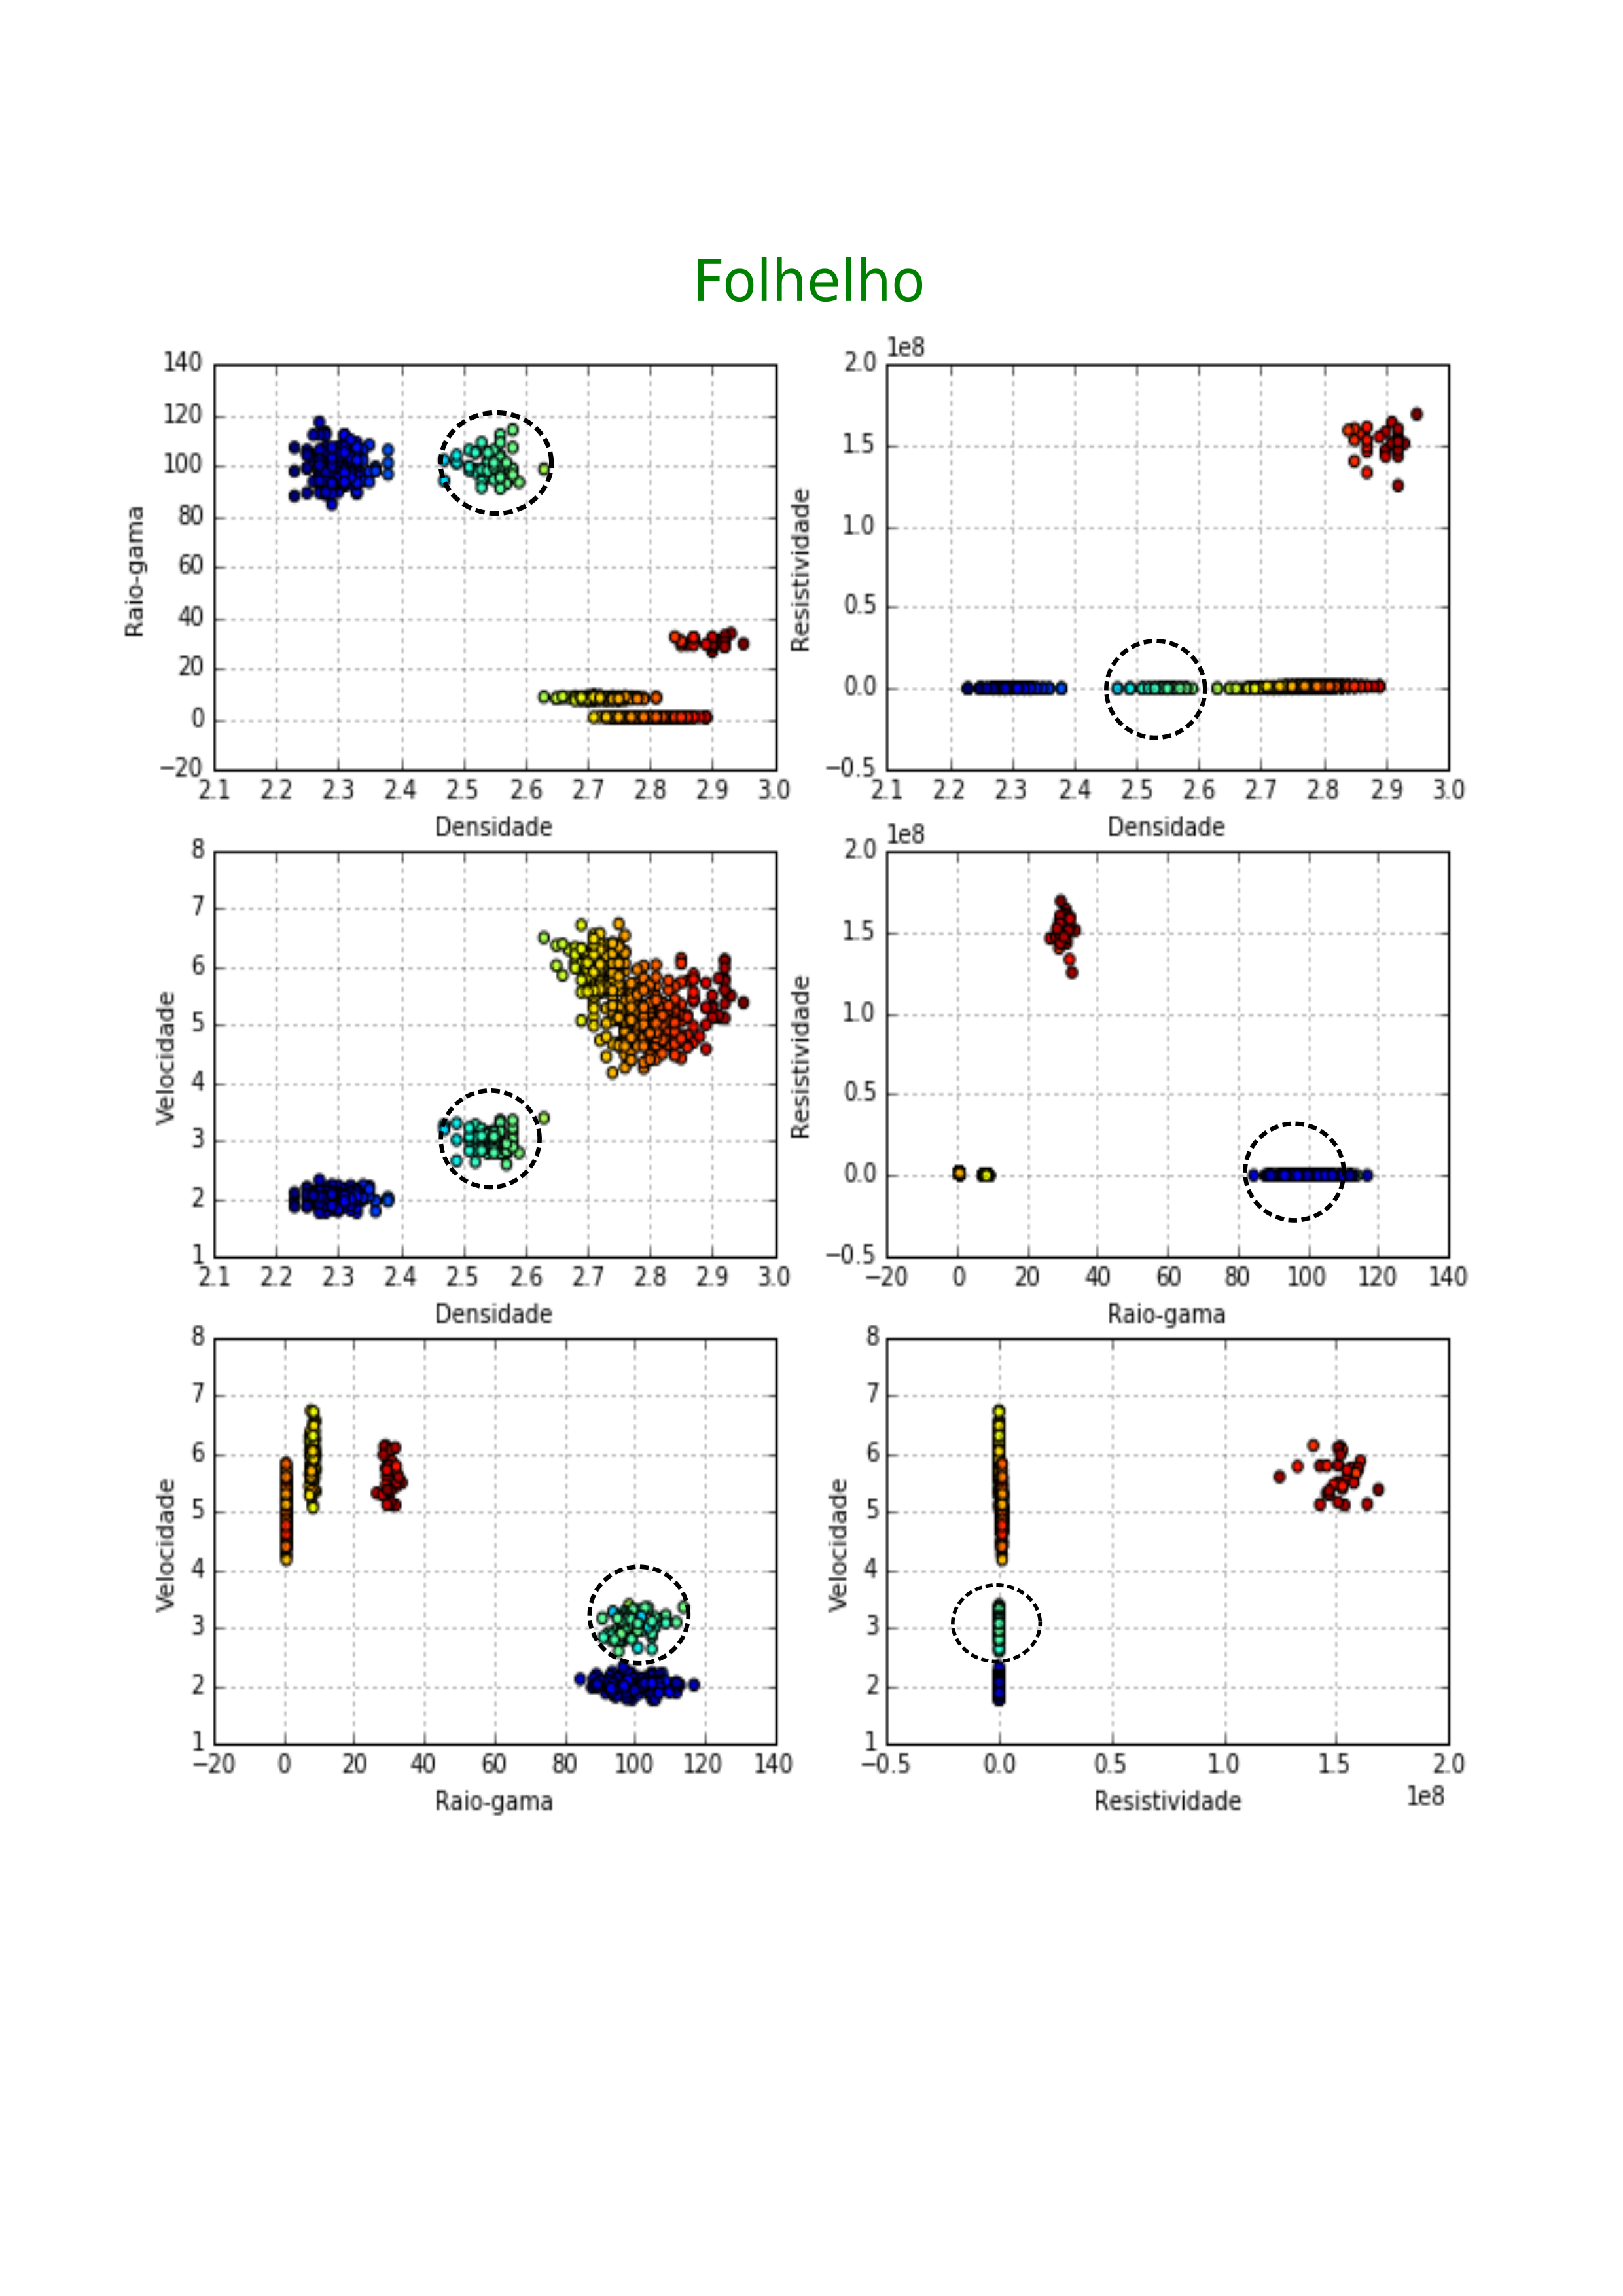
\includegraphics[scale=0.3]{Imagens/folhelhoC1.png}
		\caption{Agrupamento de dados do poço C1.}
	\end{figure} 
\end{frame}

\begin{frame}
	\frametitle{Clusterização do poço C1}
	\begin{figure}[H]
		\centering
		\includegraphics[scale=0.3]{Imagens/dolomitaC1.png}
		\caption{Agrupamento de dados do poço C1.}
	\end{figure} 
\end{frame}

\begin{frame}
	\frametitle{Clusterização do poço C1}
	\begin{figure}[H]
		\centering
		\includegraphics[scale=0.3]{Imagens/diabasioC1.png}
		\caption{Agrupamento de dados do poço C1.}
	\end{figure} 
\end{frame}

\begin{frame}
	\frametitle{Clusterização do poço C1}
	\begin{figure}[H]
		\centering
		\includegraphics[scale=0.3]{Imagens/embasamentoC1.png}
		\caption{Agrupamento de dados do poço C1.}
	\end{figure} 
\end{frame}

\begin{frame}
	\frametitle{Clusterização do poço C2}
	\begin{figure}[H]
		\centering
			\includegraphics[scale=0.3]{Imagens/cluterpocoC2.png}
		\caption{Agrupamento de dados do poço C2.}
		\label{clusterC2}
	\end{figure} 
\end{frame}

\begin{frame}
	\frametitle{Clusterização do poço C2}
	\begin{figure}[H]
		\centering
		\includegraphics[scale=0.4]{Imagens/conglomeradoC2.png}
		\caption{Agrupamento de dados do poço C2.}
	\end{figure} 
\end{frame}

\begin{frame}
	\frametitle{Clusterização do poço C2}
	\begin{figure}[H]
		\centering
		\includegraphics[scale=0.3]{Imagens/folhelhoC1.png}
		\caption{Agrupamento de dados do poço C2.}
	\end{figure} 
\end{frame}

\begin{frame}
	\frametitle{Clusterização do poço C2}
	\begin{figure}[H]
		\centering
		\includegraphics[scale=0.3]{Imagens/dolomitaC2.png}
		\caption{Agrupamento de dados do poço C2.}
	\end{figure} 
\end{frame}

\begin{frame}
	\frametitle{Clusterização do poço C2}
	\begin{figure}[H]
		\centering
		\includegraphics[scale=0.4]{Imagens/diabasioC2.png}
		\caption{Agrupamento de dados do poço C2.}
	\end{figure} 
\end{frame}

\begin{frame}
	\frametitle{Clusterização do poço C2}
	\begin{figure}[H]
		\centering
		\includegraphics[scale=0.4]{Imagens/embasamentoC2.png}
		\caption{Agrupamento de dados do poço C2.}
	\end{figure} 
\end{frame}






%%%%%%%%%%%%%%%%%%%%%%%%%%%%%%%%%%%%%%%%%%%%%%%%%%%%%%%%%%%%%%%%%%%%%%%%%%%%
%-------------------------RESULTADOS E DISCUSSÕES---------------------------------------
%%%%%%%%%%%%%%%%%%%%%%%%%%%%%%%%%%%%%%%%%%%%%%%%%%%%%%%%%%%%%%%%%%%%%%%%%%%%

\section{Resultados e Discussões}

\subsection{Treinamento}

\begin{frame}
	\frametitle{Treinamento}
	\begin{figure}
		\centering
		\includegraphics[width=7.0cm]{Imagens/SOM1_2d.pdf}
		\caption{Mapa auto-organizado (a) no primeiro ciclo de treinamento.}
	\end{figure}
\end{frame}

\begin{frame}
	\frametitle{Treinamento}
	\begin{figure}
		\centering
		\includegraphics[width=7.0cm]{Imagens/SOM5_2d.pdf}
		\caption{Mapa auto-organizado (b) no quinto ciclo de treinamento.}
	\end{figure}
\end{frame}

\begin{frame}
	\frametitle{Treinamento}
	\begin{figure}
		\centering
		\includegraphics[width=7.0cm]{Imagens/SOM100_2d.pdf}
		\caption{Mapa auto-organizado (c) no centésimo ciclo de treinamento.}
	\end{figure}
\end{frame}

\begin{frame}
	\frametitle{Treinamento}
	\begin{figure}
		\centering
		\includegraphics[width=7.0cm]{Imagens/SOM1000_2d.pdf}
		\caption{Mapa auto-organizado (d) no milésimo ciclo de treinamento.}
		\label{SOMd}
	\end{figure}
\end{frame}

\begin{frame}
	\frametitle{Treinamento}
	\begin{figure}[H]
		\centering
			\includegraphics[scale=0.23]{Imagens/conv070917.png}
		\caption{Teste de convergência da rede.}
		\label{convergencia}
	\end{figure} 
\end{frame}

\subsection{Identificação}

\begin{frame}
	\frametitle{Identificação}
\begin{figure}[H]
	\centering
		\includegraphics[scale=0.45]{Imagens/IDC1.png}
	\caption{Dado de saída da rede para o poço de classificação C1.}
	\label{Class C1}
\end{figure} 
\end{frame}

\begin{frame}
	\frametitle{Identificação}
	\begin{figure}[H]
		\centering
			\includegraphics[scale=0.45]{Imagens/IDC2.png}
		\caption{Dado de saída da rede para o poço de classificação C2.}
		\label{Class C2}
	\end{figure} 
\end{frame}
	


%%%%%%%%%%%%%%%%%%%%%%%%%%%%%%%%%%%%%%%%%%%%%%%%%%%%%%%%%%%%%%%%%%%%%%%%%%%%
%-------------------------CONCLUSÕES---------------------------------------
%%%%%%%%%%%%%%%%%%%%%%%%%%%%%%%%%%%%%%%%%%%%%%%%%%%%%%%%%%%%%%%%%%%%%%%%%%%%

\section{Conclusões}

\begin{frame}
	\frametitle{Conclusões}
\begin{small}
	

	\begin{itemize}
		\item O teste de convergência da rede indicou que o número de erros não diminui após o milésimo ciclo de treinamento;
		\pause
		\item A maior área de especialização do mapa auto-organizado usado na identificação da rede está relacionada com o padrão sino;
		\pause
		\item As propriedades físicas de densidade e raio-gama tem uma importância relativa maior, na classificação das litologias pela rede dos poços  C$1$ e C$2$ (diagramas de velocidades por densidade e o de velocidade por raio-gama);
		\pause
		\item A saída da rede aponta que o maior número de casos dos erros ocorreram em uma única classe de rocha, a do embasamento;
		\pause
		\item O menor número de erros relativos encontrados, no poço C$2$ deve-se a escolha da alocação do furo, no perfil e do poço utilizado no treinamento. O poço C$2$ localiza-se em um baixo estrutural, atingindo menos de $1$km do embasamento. Entretanto, o poço C$1$ encontra-se em um alto estrutural, divergindo do poço C$2$ e produzindo, consequentemente, os maiores erros relativos encontrados. 
	\end{itemize}
\end{small}	
\end{frame}




%%%%%%%%%%%%%%%%%%%%%%%%%%%%%%%%%%%%%%%%%%%%%%%%%%%%%%%%%%%%%%%%%%%%%%%%%%%%
%-------------------------CRONOGRAMA---------------------------------------
%%%%%%%%%%%%%%%%%%%%%%%%%%%%%%%%%%%%%%%%%%%%%%%%%%%%%%%%%%%%%%%%%%%%%%%%%%%%

\section{Cronograma}		
\begin{frame}
\begin{table}[H]

	\flushleft
	
	% definindo o tamanho da fonte para small
	% outros possíveis tamanhos: footnotesize, scriptsize
	\begin{footnotesize}
		
		% redefinindo o espaçamento das colunas
		\setlength{\tabcolsep}{1pt}
		
		% \cline é semelhante ao \hline, porém é possível indicar as colunas que terão essa a linha horizontal
		% \multicolumn{10}{c|}{Meses} indica que dez colunas serão mescladas e a palavra Meses estará centralizada dentro delas.
		\rotatebox{0}{
			\begin{tabular}{|c|c|c|c|c|c|c|c|c|c|c|c|c|c|c|c|c|c|c|c|c|c|c|c|c|}\hline
				& \multicolumn{24}{c|}{Meses}\\ \cline{2-25}
				\raisebox{1.5ex}{Etapa} & 01 & 02 & 03 & 04 & 05 & 06 & 07 & 08 & {\color{red}09} & 10 & 11 & 12 & 13 & 14 & 15 & 16 & 17 & 18 & 19 & 20 & 21 & 22 & 23 & 24 \\ \hline
				
				Pesquisa na Literatura & X & X & X & X & X & X & X & X & {\color{red}X} & X & X & X & X & X & X & X & X & X & X & X & X & X & X & X\\ \hline
				Disciplinas & & & X & X & X & X & X & X &  {\color{red}X} & X & X & X & & & X & X & X & X & X & X & X & X & X & X \\ \hline
				Formulação da Rede & & & & & & & & X &  {\color{red}X} & X & X & X & X & X & X & X & & & & & & & & \\ \hline
				Treino & & & & & & & & & & & & & X & X & X & X & X & X & X & X & X & X & X & X \\ \hline
				Resultado & & & & & & & & & & & & & & & & & & & & X & X & X & X & X \\ \hline
				Artigo 1 & & & & & & & & & & & & & & & & & & & & & & & X & X \\ \hline
				Artigo 2 & & & & & & & & & & & & & & & & & & & & & & & & \\ \hline
				Tese & & & & & & & & & & & & & & & & & & & & & & & & \\ \hline
			\end{tabular}
		}
	\end{footnotesize}
	\caption{Cronograma das atividades previstas para o primeiro biênio. Em  {\color{red}vermelho} encontra-se o mês de setembro.}
	\label{t1_cronograma}
\end{table}

\end{frame}

	
\begin{frame}
\begin{table}[H]
	\centering
	
	% definindo o tamanho da fonte para small
	% outros possíveis tamanhos: footnotesize, scriptsize
	\begin{footnotesize}
		
		% redefinindo o espaçamento das colunas
		\setlength{\tabcolsep}{1pt}
		
		% \cline é semelhante ao \hline, porém é possível indicar as colunas que terão essa a linha horizontal
		% \multicolumn{10}{c|}{Meses} indica que dez colunas serão mescladas e a palavra Meses estará centralizada dentro delas.
		\rotatebox{0}{
			\begin{tabular}{|c|c|c|c|c|c|c|c|c|c|c|c|c|c|c|c|c|c|c|c|c|c|c|c|c|}\hline
				& \multicolumn{24}{c|}{Meses}\\ \cline{2-25}
				\raisebox{1.5ex}{Etapa} & 25 & 26 & 27 & 28 & 29 & 30 & 31 & 32 & 33 & 34 & 35 & 36 & 37 & 38 & 39 & 40 & 41 & 42 & 43 & 44 & 45 & 46 & 47 & 48 \\ \hline
				
				Pesquisa na Literatura & X & X & X & X & X & X & & & & & & & & & & & & & & & & & & \\ \hline
				Disciplinas & & & & & & & & & & & & & & & & & & & & & & & & \\ \hline
				Formulação da Rede & & & & & & & & & & & & & & & & & & & & & & & & \\ \hline
				Treino & & & & & & & & & & & & & & & & & & & & & & & & \\ \hline
				Resultado & & X & X & X & X & X & X & X & & & & & & & & & & & & & & & & \\ \hline
				Artigo 1 &X & X & X & X &X & X& X& & & & & & & & & & & & & & & & & \\ \hline
				Artigo 2 & & & & & X & X & X & X & X &X & X& X& X& X& X& X& X& & & & & & & \\ \hline
				Tese & & & & & & & & & & & & & X&X & X & X & X & X & X & X & X & & & \\ \hline
				
			\end{tabular}
		}
	\end{footnotesize}
	\caption{Cronograma das atividades previstas para o segundo biênio.}
	\label{t2_cronograma}
\end{table}

\end{frame}	
	
	
\section{Bibliografia}
	\begin{frame}[allowframebreaks]{Bibliografia}
	%\frametitle{Bibliografia}
	\beamertemplatetextbibitems
	\tiny
	\bibliographystyle{apalike}
	\bibliography{references.bib}
	\end{frame}

\makeatother
{\nologo
\begin{frame}
%\titlepage
\begin{figure}
\includegraphics[scale=0.25]{Imagens/logonvertical.jpg}
\end{figure}
\begin{center}
\begin{minipage}{0.77\textwidth}
\small
\begin{center}
Rua General José Cristino, 77 CEP 20921-400\\
Rua General Bruce, 586 CEP 20921-030\\
Bairro Imperial de São Cristóvão, Rio de Janeiro - RJ\\
PABX: 55 21 3504-9100\\
\url{www.on.br}
\end{center}
\end{minipage}
\end{center}
\end{frame}
}
\end{document}
